\documentclass[10pt]{article}
\usepackage[margin=0.9in]{geometry}
\usepackage{fontspec}
\directlua{luaotfload.add_fallback("aereadfallback", {"STIX Two Math:mode=harf;", "Apple Symbols:mode=harf;", "Helvetica Neue:mode=harf;",
  "Arial Unicode MS:mode=harf;"})}
\setmainfont{Times New Roman}[RawFeature={fallback=aereadfallback}]
\setsansfont{Helvetica Neue}[RawFeature={fallback=aereadfallback}]
\setmonofont{Menlo}[Scale=0.85, RawFeature={fallback=aereadfallback}]
\usepackage{amsmath,amssymb}
\usepackage{graphicx,booktabs,longtable,array,calc,multirow,xcolor,tikz,caption,etoolbox}
\AtBeginEnvironment{longtable}{\footnotesize\setlength{\tabcolsep}{4pt}\sloppy}
\setlength{\emergencystretch}{3em}
\usetikzlibrary{arrows.meta}
\usepackage[round,authoryear]{natbib}
\usepackage[hidelinks]{hyperref}
\setcounter{secnumdepth}{2}
\captionsetup{font=small,labelfont=bf}
% pandoc's helpers
\providecommand{\tightlist}{\setlength{\itemsep}{0pt}\setlength{\parskip}{0pt}}
\makeatletter
\newsavebox\pandoc@box
\newcommand*\pandocbounded[1]{\sbox\pandoc@box{#1}\ifdim\wd\pandoc@box>\linewidth\resizebox{\linewidth}{!}{#1}\else#1\fi}
\makeatother
% the sources' own macros
\newcommand{\code}[1]{\texttt{#1}}
\newcommand{\qcref}{Section~\ref{sec:qc}}
\newcommand{\casesref}{Section~\ref{sec:cases}}
\renewcommand{\arraystretch}{1.12}
\newcolumntype{P}[1]{>{\raggedright\arraybackslash}p{#1}}
\title{AERead: Evaluating Economic Decisions in Interactive Environments}
\author{Chenyu Li \hspace{3em} Zeyu Sun \\[3pt] {\small contact@aeread.org}}
\date{Research working paper, version 15.37, 21 October 2026. Preliminary results; feedback and contributions welcome.}

\begin{document}
\maketitle
\section*{Abstract}

AI agents are increasingly asked to make economic decisions for a
principal, such as whom to trade with, what to verify and when to commit. Here a completed
transaction can destroy value and a refusal can be correct, so
task-completion or agreement scores cannot tell whether an agent served its
principal. We present AERead, an environment that scores
these decisions by the value an agent obtains. Each case defines a
distribution of economic worlds, seats with private information,
counterparts with their own interests, and a reference policy whose access
to information is stated, so that a shortfall separates poor decisions from
information the agent never had. One runtime executes every case and recomputes
each score from the sealed record without a model; quality control runs over
populations of worlds, not single tasks. We build cases in housing, procurement, data-center contracting
and refunds on this runtime. The counterpart is
part of the measurement: one agent's earnings lead over another is 42\% of
the value available in a deal head to head and 7\% against the same scripted
counterpart. Shortfalls are broken down by stratum and by action
class; in housing, nearly all of the gap to the reference falls in worlds
where the tenant's favourite listing is a lemon. Of 25 defects selected from
our quality-control record, 14 were invisible in any one world. Housing now
passes four of the five quality-control gates and no case passes all five,
so the results compare named agents on stated worlds rather than rank models. AERead's code is open source: a
new case supplies its economic rules, worlds and reference, and inherits
the runtime, replay and the quality-control standard.

% Sections 1--3, drafting pass 16 October 2026.
% Empirical scope follows the merged Sections 4--6 review snapshot.
\section{Introduction}
\label{sec:introduction}

An agent buying on behalf of a firm must decide more than whether it can
place an order. It must choose whom to trust, whether another test is worth
its cost, and when to commit before an offer expires. A tenant faces the
same problem when inspecting a home; a negotiator faces it when exchanging
price for contractual risk. In these settings, completing a transaction
can destroy value, while refusing it can be the right decision. We use
\emph{economic-agent readiness}, the quantity AERead's name refers to, to
mean an agent's ability to obtain value for a principal within a stated
mandate, given limited information and other parties' interests. AERead
measures this ability in stated worlds against stated references;
readiness for deployment in a particular firm is a further question that
these measurements inform but do not settle.

Evaluating this ability requires a reference for what the agent could
have achieved. A good realized outcome can follow a poor decision, and a
shortfall from a fully informed optimum can reflect information the agent
never had. The counterpart also matters: a strategy that succeeds against
a cooperative seller may fail against a different policy. Existing work
provides interactive task evaluation and economic decision benchmarks
\citep{merrill2026terminalbench,fish2025econevals,zhang2026termsbench}.
The problem we address is how to make information, counterpart behavior
and reference values explicit across different economic cases, then test
whether the resulting scores measure the intended decisions.

AERead is an environment for constructing and evaluating such cases.
Each case specifies the parties, their observations and legal actions,
the world distribution, and checks on behavior and outcomes. A shared
runtime executes play and records evidence. Case-specific references give
scores an economic interpretation, and results keep their native units.

\begin{figure}[htbp]\centering\renewcommand{\thefigure}{1.1}
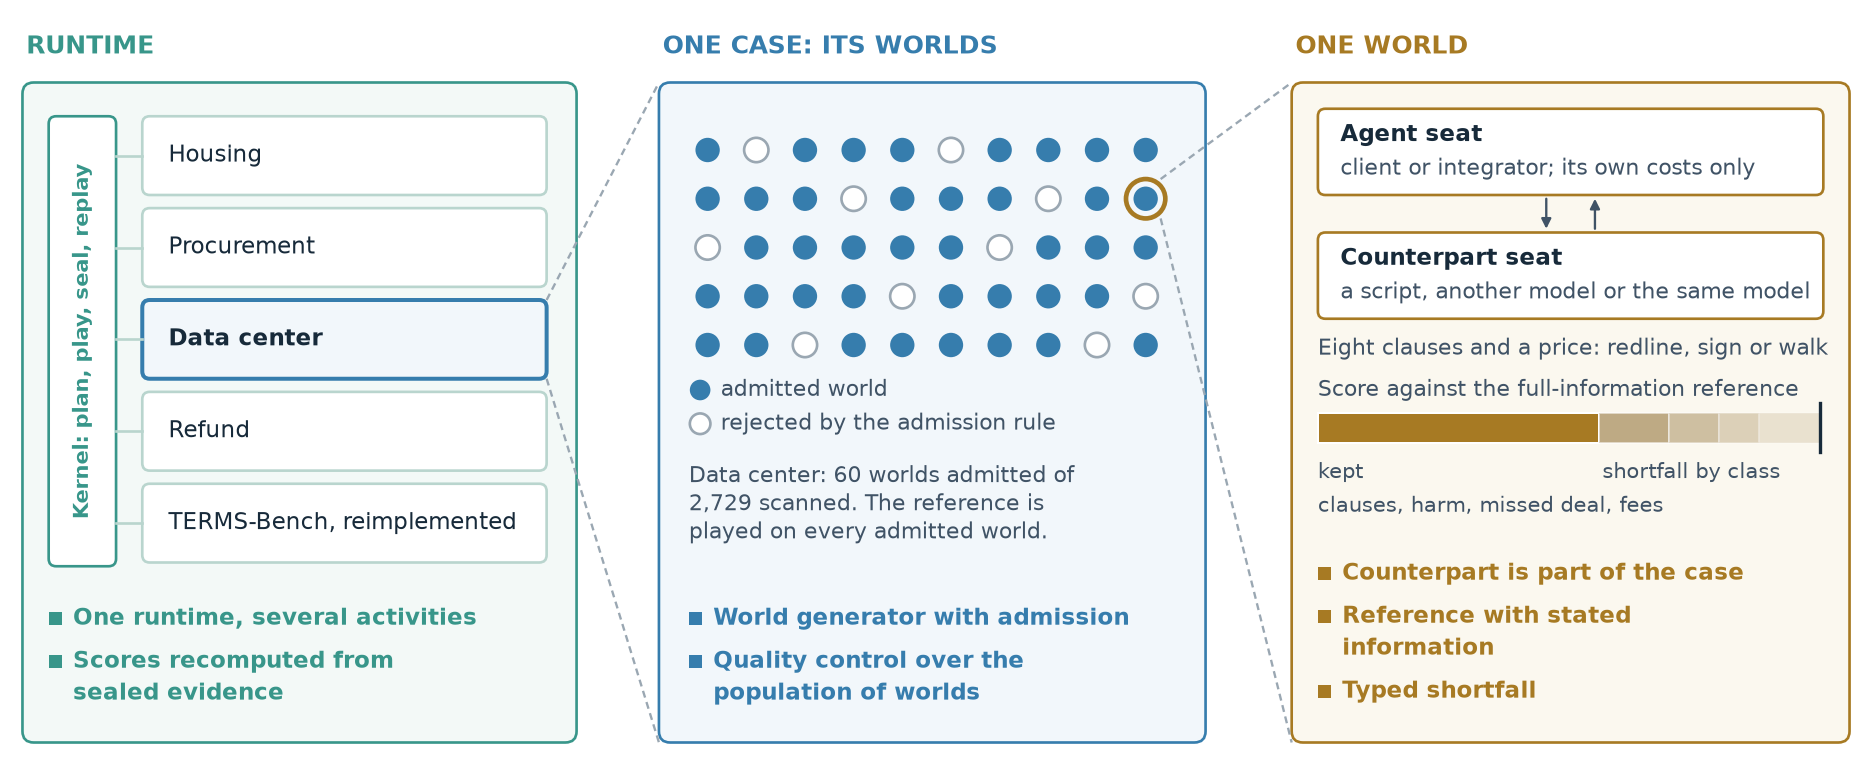
\includegraphics[width=\linewidth]{figures/evaluation_levels.png}
\caption{\textbf{The three levels of an AERead evaluation,} with the Data-center agreement as the example. The runtime hosts several case families (left). A case draws a population of worlds and admits those where the decision matters; quality control runs over that population (centre). In one world, the agent holds a seat, a counterpart holds another, and the score is compared with the case reference and split into shortfall classes (right). Dashed lines mean ``contains'', not a sequence. Each panel lists the properties of Section~1 that belong to its level. The dot pattern and the score bar are schematic.}
\label{fig:case}
\end{figure}


AERead combines seven properties, several of which appear in prior
benchmarks (Table~2.1, which we graded ourselves from each paper's
description of its method). The first three
properties concern a single world, the next two a case's population of worlds, and the
last two the runtime (Figure~1.1). We built each of them and applied it to the
cases reported here.
\begin{enumerate}
\item \textbf{Value against a reference with stated information.} Scores
are economic values in each case's own units, measured against a feasible
policy, the best policy given the deciding seat's information, or a
labelled full-information bound. We play each reference through the
environment on every included world (Section~\ref{sec:qc}).
\item \textbf{The counterpart is part of the case.} Other parties are seats
with their own information and interests, played by scripted policies,
another model or the same model, and each claim names its counterpart. In
the Data-center case, the measured gap between two agents depends strongly on
which counterpart they face, even when each transfer between them is counted once
(Section~\ref{sec:cases}).
\item \textbf{Typed shortfall.} The gap to the reference is split into
observed action classes, such as tests not taken, worse terms, harmful
agreements and negotiation fees, so a result states where value was lost
as well as how much (Section~\ref{sec:cases}).
\item \textbf{World generators with an inclusion criterion.} A case is a generator of
worlds, and its evaluation sets regenerate from their seeds. An inclusion criterion,
computed before any agent plays, keeps only worlds in which simple
shortcuts lose a stated margin. The Data-center comparison, for example, used 80
worlds included from 5,436 scanned (Section~\ref{sec:cases}).
\item \textbf{Quality control over populations of worlds.} Cases are
qualified through quality-control gates (Section~\ref{sec:qc}). We score simple-rule ceilings beside the
agents and audit the task prompts. More than half of the defects we selected
from our record were invisible in any single world.
\item \textbf{Scores recomputed from sealed evidence.} The kernel hashes a
plan before execution, seals the events, and replays each receipt to
recompute its scores without calling a model; no model judges a score
(Section~\ref{sec:runtime}).
\item \textbf{One runtime for several activities.} Families supply only the
economic rules. Four cases and a reimplementation of three
TERMS-Bench counterpart families run on the same kernel; the
reimplementation's reproduction is still in progress (Appendix~E.10).
\end{enumerate}
A researcher studying another economic decision therefore writes only its
rules, worlds and reference. Execution, sealing, replay, counterpart seats
and the quality-control gates come with the runtime, so a new case starts
with the same evidence and checks as the existing ones.
Sections 3 and 4 describe the case design and the runtime, Section 5 the
cases, and Section 6 the quality control. Section 7 states what the results
do and do not establish.

\section{Related work}
\label{sec:related-work}

Table~2.1 compares the closest benchmarks on the seven properties of
Section~\ref{sec:introduction}; the paragraphs below discuss them by theme.

\begin{table}[htbp]\centering\small\renewcommand{\thetable}{2.1}
\caption{\textbf{The seven properties in related benchmarks,} read from each paper's description of its own method: $\bullet$ present, $\circ$ partly present, -- absent. Columns: 1. Value against a reference with stated information; 2. Counterpart is part of the case; 3. Typed shortfall; 4. World generator with admission; 5. Quality control over populations of worlds; 6. Scores recomputed from sealed evidence; 7. Several economic activities on one runtime. Each cell was read against a written definition, and the lower mark was chosen where a reading was borderline; page references for every cell are kept with the source. AERead's row describes the cases reported here; Housing v15 passes four of the five qualification gates and none passes all five (Section 6). TERMS-Bench has five of the seven properties in full. AERead adds several activities on one runtime and, in three of its cases, an admission rule that screens shortcuts.}
\label{tab:comparison}
\begin{tabular}{lccccccc}
\toprule
Benchmark & 1 & 2 & 3 & 4 & 5 & 6 & 7 \\
\midrule
Terminal-Bench & -- & -- & $\circ$ & $\circ$ & $\bullet$ & $\circ$ & $\circ$ \\
τ²-bench & -- & $\circ$ & $\circ$ & $\circ$ & $\circ$ & $\circ$ & $\circ$ \\
GDPval & -- & -- & $\circ$ & -- & $\circ$ & -- & $\circ$ \\
Agents' Last Exam & -- & -- & $\circ$ & $\circ$ & $\circ$ & $\circ$ & $\circ$ \\
EconEvals & $\bullet$ & -- & $\circ$ & $\circ$ & $\circ$ & $\circ$ & $\bullet$ \\
NegotiationArena & $\circ$ & $\bullet$ & $\circ$ & -- & -- & $\circ$ & $\circ$ \\
AgenticPay & $\circ$ & $\bullet$ & $\circ$ & -- & -- & $\circ$ & $\circ$ \\
TERMS-Bench & $\bullet$ & $\bullet$ & $\bullet$ & $\circ$ & $\bullet$ & $\bullet$ & $\circ$ \\
AERead (this paper)$^{*}$ & $\bullet$ & $\bullet$ & $\bullet$ & $\circ$ & $\bullet$ & $\bullet$ & $\bullet$ \\
\bottomrule
\end{tabular}
\end{table}


\paragraph{Economically valuable work.}
GDPval selects professional tasks by occupation and evaluates deliverables
through expert comparison \citep{patwardhan2025gdpval}. Agents' Last Exam
(ALE) evaluates expert-authored professional workflows with task-specific
verification \citep{sun2026agentslastexam}. AERead evaluates decisions
under a principal's mandate, with responsive counterparts and payoff
references that specify the deciding party's information.

\paragraph{Interactive agent evaluation.}
Terminal-Bench verifies final environment state and supplies human-written
solutions \citep{merrill2026terminalbench}. AppWorld combines an application
engine with state-based evaluation, including collateral-change checks
\citep{trivedi2024appworld}. τ²-bench lets agent and user act on shared
state \citep{barres2025tau2}.

\paragraph{Economic decisions and negotiation.}
EconEvals covers procurement, scheduling, pricing and economic choice
\citep{fish2025econevals}. NegotiationArena studies bargaining tactics
\citep{bianchi2024negotiationarena}; SidConArena combines negotiation,
production and auctions \citep{feng2026sidconarena}. AgenticPay evaluates
buyer--seller bargaining under private reservation values, scoring
agreement, surplus allocation and speed \citep{liu2026agenticpay}.
TERMS-Bench specifies counterpart types, policies and payoffs to diagnose
negotiation through oracle-reference gaps \citep{zhang2026termsbench}; our
case specifications follow its decomposition into environment, protocol
and counterpart policy (Appendix~A), and Appendix~E.10 reports a
reimplementation of three of its counterpart families on AERead's runtime.
AERead retains case-specific payoff units, distinguishes full-information
bounds from information-constrained policy references, and applies quality control to world
distributions and measurement paths.

\paragraph{Shared environments and evaluation quality.}
OpenSpiel and PettingZoo provide common interfaces for games and
multi-agent environments \citep{lanctot2019openspiel,terry2021pettingzoo}.
AERead similarly separates shared execution from case semantics
(Appendix H). Terminal-Bench combines executable reference solutions,
automated checks, human review and adversarial exploit testing
\citep{merrill2026terminalbench}. The Agentic Benchmark Checklist
identifies task and reward defects that distort performance
\citep{zhu2025abc}. Our QC analysis tests whether prompts, controls and
counterpart assignments support valid comparisons across distributions
of economic worlds.

\section{Task design and construction}
\label{sec:task-design}

Three of AERead's properties are fixed when a case is designed: the
reference and the information it may use, the counterpart seats, and the
world generator with its inclusion criterion.

\subsection{Cases, worlds and seats}
\label{sec:task-formulation}

A \emph{case} defines an economic decision problem; a \emph{world} is
one instance of that design, with particular valuations, private types,
costs and deadlines. A \emph{seat} is a party's position in the
interaction, with its own objective, information and permitted actions.
A policy occupies a seat and chooses actions from its observations and
available history. The family implementation supplies the environment,
observation rules, legal actions, transitions and verifier.

For example, Housing places a tenant among four listings with hidden
quality. The tenant can inspect, make offers and decide whether to sign;
landlord replies and outside demand affect the opportunities that remain.
Inspection changes both information and cost. The verifier therefore
needs to distinguish a legal action, a favorable realized outcome and a
good decision given the tenant's information.

In a controlled comparison, the evaluated policy occupies one seat and
counterparts follow fixed policies. Cross-play and self-play change those
assignments and answer different questions. Each comparison names the
seat, counterpart configuration and world distribution to which it
applies. Appendices A--D give the case specifications, counterpart
policies, references and measures.

\subsection{Selecting economic decisions}

We organize coverage around activities in which a party's choices affect
the value of a transaction \citep{li2026activities}. A candidate case
needs a consequential decision, a counterpart with its own interests and
information, and an outcome that can be evaluated inside the world.
The intended coverage spans business purchases, labour contracts, capital
and corporate transactions, household purchases, and public purchases.
Contractual terms, risk allocation and disputes enter as decisions within
these transactions.

The four examples cover business and household purchases. They were
selected to exercise different references and counterpart configurations;
they are not a representative sample of economic activity. Economic
stakes motivate which decisions to study, but the reported scores are
case-specific quantities, without a cross-family aggregate or an estimate
of economy-wide gains.

\subsection{Constructing and qualifying a case}
\label{sec:case-construction}

A contribution begins with a decision and an interpretation of success.
The case author specifies the principal's objective and constraints, what each
seat can observe, which actions commit resources, and how counterpart
policies respond. The task prompt must state the rules needed to make the
decision while preserving the intended private information. These
choices define the mechanism that a score is meant to test.

The author then provides a world generator or a fixed evaluation set, an inclusion
criterion, and a reference whose access to information is explicit. The inclusion criterion
screens each candidate world before any agent plays and before hidden
types are drawn. It is computed exactly from the public world and the stated
prior. It keeps a world only if simple shortcuts, such as accepting the
default terms or ignoring private information, fall short of the reference
by a stated margin. Whether the reference can be reached is a separate
check. Executable controls play the reference through the actual environment and
verifier on every included world. Simple policies are played beside it, to reveal
shortcuts or ceiling effects that the screen missed. The evaluation set must also be
valid, free of duplicates, and split into disjoint development and holdout
ranges. A full-information bound is labelled separately from a policy
the evaluated seat could execute. The case states its score units,
the direction of each score, and its treatment of invalid actions and incomplete episodes.

Before a confirmatory comparison, the campaign freezes the worlds,
seat assignments, prompts, agent settings, budgets and analysis, and pre-registers them. Its
evidence package should connect each reported measure to the retained
actions and outcomes, the scoring implementation, and a command that
reproduces it. Section 4 describes the shared execution path. The current drivers
and headline analyses extend beyond what a receipt covers in places, which
Appendix H records.

This is the contribution and qualification standard. The four examples meet it
to different degrees: their implementation support and completed checks vary
(Section 6). Cases can be useful for development before
qualification, provided their reports identify missing checks, preserve
failed attempts, and distinguish analyses pre-registered before execution from
later corrections. The current examples demonstrate the workflow and
its failure modes; they do not establish successful adoption by external
contributors.

% Revision 10. Concise main text; technical contract retained in appendix.
% Runtime baseline: dec1a40f. Evidence review dated 2026-10-14.
\section{Shared runtime and evaluation harness}
\label{sec:runtime}
\label{sec:measurement}

The runtime provides two of AERead's properties: one kernel executes every
family, and every score is recomputed by code from sealed evidence. The
shared runtime, or \emph{kernel}, executes the case designs in
Section~\ref{sec:task-design}. Families supply the economic rules;
the kernel schedules play and records the evidence used for evaluation
(Figure~\ref{fig:architecture}).

\begin{figure}[htbp]\centering\renewcommand{\thefigure}{4.1}
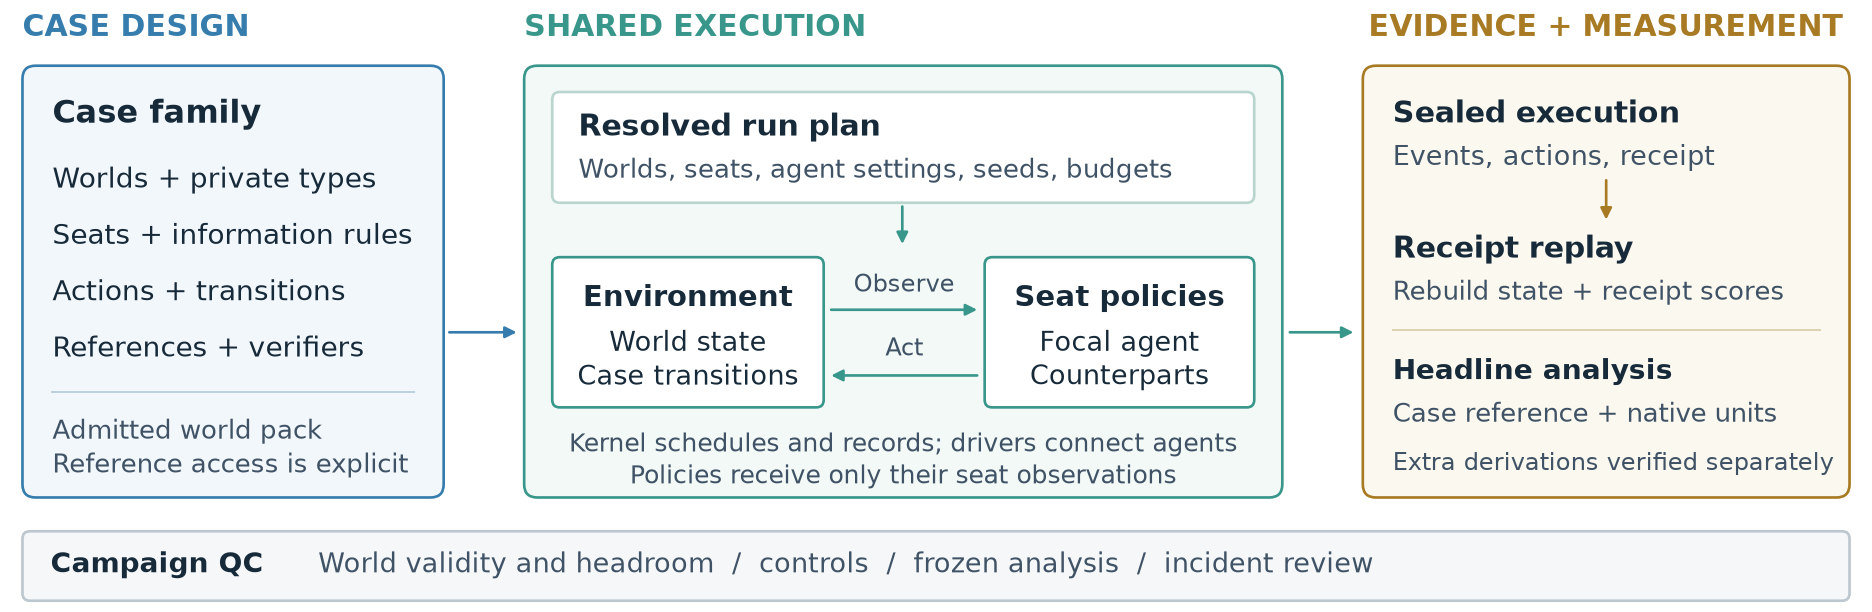
\includegraphics[width=\linewidth]{figures/architecture_overview.png}
\caption{\textbf{AERead architecture.} Families define the economic world and reference; the runtime coordinates seat policies and retains execution evidence. Agents receive only their seat observations, while scoring uses explicitly declared reference access. Replay checks receipt consistency; separate headline derivations require their own verification. Applied coverage and QC verdicts vary by campaign (Appendices F and H).}
\label{fig:architecture}
\end{figure}


\subsection{Verification}
Checks compare behavior or outcomes against five kinds of reference.
An \emph{answer key} specifies a correct resolution, and a \emph{rule}
specifies a constraint. A \emph{value} reference measures economic outcomes against
a policy or a bound, a \emph{relative} reference compares named agents or populations,
and a \emph{rubric} rates an artifact. Each check states its output
(pass/fail, count or amount) and whether it concerns the outcome or
the path. Results retain their native units, and we report no cross-family
aggregate. Value references distinguish a reachable policy, the best
policy given the decider's information, and a full-information upper
bound; the last need not be attainable by the evaluated seat.

The case-study scores are computed by code. Kernel replay reconstructs
state and each receipt's score from recorded actions without calling a
model. Housing and Procurement also report separately verified headline measures computed
outside that receipt certificate; their measurement paths are documented
in Appendix~\ref{app:runtime-cases}. Replay establishes consistency with
recorded execution. Scientific qualification depends on the checks in
\qcref{}; none of the four current designs passes all of the quality-control Gates~1--5
in the snapshot we review.

\subsection{Evaluation harness}
Before execution, the kernel hashes a plan that specifies the worlds, seat
assignments, agent configurations, seeds and budgets. During simultaneous
play, it freezes all acting seats' observations before requesting actions
and then applies their joint transition. Calls through its provider and
tool interfaces are logged with typed outcomes. Finalization seals the
evidence and produces a receipt binding the plan, world and scores.

A seat is played in one of three ways. Most models run through AERead's
own harness. Each action is a single call through a pinned provider route:
the call receives the seat's instructions and its current observation and returns one action
in the case's schema, with no tools and no memory beyond what the
observation shows. The harness checks the route against its pin, requests a
seed, and records the specified reasoning setting and output limit.
Gemini 3.8 Flash, GLM 5.3 Flash and GPT-6 Luna in Housing (Gemini and Luna
in Procurement), the Refund models and the TERMS-Bench agents are run this
way. The two frontier agents, Opus 5.5 and Sol 6.1, run instead through
their vendors' command-line tools, Claude Code and Codex. Each action starts a fresh process
at low reasoning effort, with the same instructions and schema, tools
disabled or refused, and no session carried over. Neither tool was fully
isolated from the operator's machine (Table~\ref{tab:cli-controls}):
Claude Code ran in safe mode, with none of the operator's instructions,
memory or skills but with its working directory in context, and Codex
still listed eight of the operator's own skills. Only the tool's version
and binary are checked, and the tool exposes no seed, temperature or output
limit. Through the harness, the system under evaluation is the model; through a
command-line tool, it is the product, including the tool's own instructions and
internal turns. A comparison across the two paths therefore compares agent
configurations rather than models, and each result names its path.
Counterparts, references and simple-rule baselines are scripted, call no
model and replay exactly. A recorded setting does not establish that a
provider honoured it; Appendix~\ref{app:runtime} gives the controls each
path applied and the versions behind each reported panel.

\section{Case studies}\label{case-studies}\label{sec:cases}

We present four cases that we built as maintainers (Table 5.1). They are worked examples of the framework rather
than a fixed benchmark: each is a starting point for questions about the decision it models, and Section 7.2 lists
the questions we consider open. The cases show how the counterpart changes measured value and how a shortfall divides
into typed action classes, and Section 5.3 runs an external benchmark on the same runtime. We describe Housing,
Procurement and Data center here and specify them in Appendices A--D; Refund appears only in the cross-case comparison.
Each case is a family rather than a fixed task set. It consists of a generator of worlds; a case-specific reference,
which is either a policy that uses only what the deciding side may know or an explicitly labelled full-information
upper bound; an inclusion criterion that keeps the worlds in which the decision matters (its form varies by case;
Appendix E.2); and a set of verifiers. The references differ in what a shortfall means. Against a reachable policy,
the shortfall is the value that a feasible strategy would have kept. Against the best policy given the decider's
information, it is the whole cost of the decisions. Against a full-information bound, it also includes the value of
information that no seat had (Appendix C).

We choose cases by the economic value of the decision rather than by occupation \citep{li2026activities}. An activity qualifies when its
value is decided rather than produced, when a counterparty has its own interest and private information, and when the
result can be scored within a world against a computed reference. The four examples lie in two of the five
transaction classes introduced in §3, business and household purchases. We chose them to span the kinds of verifier
and counterpart, not to sample a representative distribution.

\renewcommand{\thetable}{5.1}
\begin{longtable}[]{@{}
  >{\raggedright\arraybackslash}p{(\linewidth - 8\tabcolsep) * \real{0.2000}}
  >{\raggedright\arraybackslash}p{(\linewidth - 8\tabcolsep) * \real{0.2000}}
  >{\raggedright\arraybackslash}p{(\linewidth - 8\tabcolsep) * \real{0.2000}}
  >{\raggedright\arraybackslash}p{(\linewidth - 8\tabcolsep) * \real{0.2000}}
  >{\raggedright\arraybackslash}p{(\linewidth - 8\tabcolsep) * \real{0.2000}}@{}}
\caption{\textbf{The four cases. Each case is scored in its own units against the reference given in the last column.}}\label{tab:5.1}\tabularnewline
\toprule\noalign{}
\begin{minipage}[b]{\linewidth}\raggedright
Case
\end{minipage} & \begin{minipage}[b]{\linewidth}\raggedright
Real setting
\end{minipage} & \begin{minipage}[b]{\linewidth}\raggedright
What the agent decides
\end{minipage} & \begin{minipage}[b]{\linewidth}\raggedright
Who it faces
\end{minipage} & \begin{minipage}[b]{\linewidth}\raggedright
Scored against
\end{minipage} \\
\midrule\noalign{}
\endhead
\bottomrule\noalign{}
\endlastfoot
Housing & informal rental listings & which listing to inspect, what to offer, and whether to sign when some listings are lemons & scripted landlords; other tenants take listings it leaves & a scripted tenant that uses only what the tenant knows \\
Procurement & wholesale sourcing & pay more for an established supplier, or test a cheaper newcomer, before a deadline & scripted suppliers & the best plan given what the buyer knows, solved exactly \\
Data center & AI-infrastructure contracting & which risk clauses to change, what price to name, and when to sign or walk away & the other side: a script, another model or the same model & the best agreement at both sides' true costs, which neither side knows \\
Refund & customer refund claims & what to ask, decide and pay on a claim under a written policy & the other parties to the claim, scripted & a hand-written correct resolution \\
\end{longtable}

We report how much room each case leaves as a share of that case's own reference value. Tables 5.2 to 5.4 give each
subject's result and gap in this form, and Figure 5.2 divides the gap by action class in the case's own units. The
cases use four of the kinds of check defined with the runner's measurement layer (§4): an answer key, stated rules,
the value of the best policy or a bound, and relative standing against another agent. None uses a rubric. Every score
is computed by code, with no model in the loop. The kernel's replay recomputes each receipt's own score from its
sealed events, whereas the headline measures of Housing and Procurement are computed by case code outside that
certificate (Appendix F.2). Table E.1 lists every check.

\subsection{Results}\label{results}

Each result below is bounded by its case's quality-control gates; Table 6.1 gives every comparison's status, and
Section 6 describes the gates. ``Pre-registered'' below describes how a comparison was run, namely with its analysis
committed to the repository before any episode; it does not describe the case. The results compare the named
subjects on these worlds and are not qualified benchmark scores.

\textbf{Housing.} The structure follows informal rental markets on social platforms such as RedNote. Listings are posted
with photos that a tenant cannot check before viewing, a viewing costs time, and good listings are often taken while
the tenant decides. We set the rents, the lemon share and the inspection cost ourselves; they are not drawn from
platform data. A tenant chooses among four listings, two of which are lemons. It knows its own value v\_ℓ for each
listing if sound, but not which two are lemons; each of the six pairs is equally likely. In each of three rounds it
may pay \$25 to inspect one listing, make one offer, and sign or walk away from a lease it is offered, while each
listing it did not bid on is taken by outside demand with probability ½. Signing listing ℓ at rent x after k
inspections pays

\[ \text{v\_ℓ − 1,000·𝟙[ℓ is a lemon] − x − 25k,} \tag{1} \]

and signing nothing pays −25k. The difficulty lies in information. A listing worth \$400 more than its ask if sound is
worth 400 − ½·1,000 = −\$100 if signed blind at the ask, but ½·400 − 25 = +\$175 if it is inspected first and signed only
when sound; inspecting a second listing takes another round, in which each listing not bid on may be taken. A
landlord's reply can reveal a lemon at no cost: every world is played against one landlord kind whose reply to a low
offer reveals a lemon and one whose reply does not. We score a blind signing at its expected value given what the
tenant knew, so that the score follows the decision rather than the draw, with the odds conditioned on every
informative landlord reply. This corrected measure is introduced in this paper; v14's pre-registered measure
conditioned on only one landlord kind (Appendix E.4). The comparison reported here, v15, was pre-registered before any
of its artifacts and changes four things from v14. Each included world is screened so that the best informed tenant
beats a simple inspect-then-sign rule by at least \$25 (119 of 437 candidate main worlds failed); the tenant's task
prompt states how landlords price; the corrected measure is primary from the start; and each receipt scores the
deciding tenant. Its holdout of 40 worlds changes one mechanism, outside demand at 0.3 a round, and its task prompt
says so.

\renewcommand{\thetable}{5.2}
\begin{longtable}[]{@{}
  >{\raggedright\arraybackslash}p{(\linewidth - 8\tabcolsep) * \real{0.1579}}
  >{\raggedleft\arraybackslash}p{(\linewidth - 8\tabcolsep) * \real{0.2105}}
  >{\raggedleft\arraybackslash}p{(\linewidth - 8\tabcolsep) * \real{0.2105}}
  >{\raggedleft\arraybackslash}p{(\linewidth - 8\tabcolsep) * \real{0.2105}}
  >{\raggedleft\arraybackslash}p{(\linewidth - 8\tabcolsep) * \real{0.2105}}@{}}
\caption{\textbf{Housing v15, main evaluation set of 260 worlds (200 with the favourite a lemon, 60 sound): seat 0's net payoff under the corrected measure as a share of what the best informed tenant earns in the same worlds (\$307 a world on the main evaluation set), averaged over the two landlord arms. Differences are in percentage points of that value, with 95\% intervals over worlds. The comparison was pre-registered before any v15 artifact; dollar values are in the results note, and the comparison with v14 is in Table E.13. Sol 6.1 and Opus 5.5 played the same worlds through their command-line tools in a pre-registered addendum, outside v15's contrasts.}}\label{tab:5.2}\tabularnewline
\toprule\noalign{}
\begin{minipage}[b]{\linewidth}\raggedright
\end{minipage} & \begin{minipage}[b]{\linewidth}\raggedleft
Gemini 3.8 Flash
\end{minipage} & \begin{minipage}[b]{\linewidth}\raggedleft
GPT-6 Luna
\end{minipage} & \begin{minipage}[b]{\linewidth}\raggedleft
Sol 6.1 (Codex), addendum
\end{minipage} & \begin{minipage}[b]{\linewidth}\raggedleft
Opus 5.5 (Claude Code), addendum
\end{minipage} \\
\midrule\noalign{}
\endhead
\bottomrule\noalign{}
\endlastfoot
Share of the best informed tenant's value & 78.7\% & 62.9\% & 90.4\% & 80.4\% \\
Favourite is a lemon / sound & 68.8\% / 100.0\% & 46.8\% / 97.3\% & 85.9\% / 100.0\% & 71.2\% / 100.0\% \\
Minus \texttt{inspect\_\allowbreak{}then\_\allowbreak{}sign} (the pre-registered beatability baseline), points & +29.3 {[}+24.7, +33.8{]} & +13.4 {[}+8.2, +18.6{]} & +40.9 {[}+36.2, +45.6{]} & +30.9 {[}+26.3, +35.5{]} \\
Minus \texttt{inspect\_\allowbreak{}lowball} (v14's reachable reference), points & −16.6 {[}−20.8, −12.5{]} & −32.5 {[}−37.8, −27.3{]} & −5.0 {[}−8.0, −2.0{]} & −15.0 {[}−18.9, −11.0{]} \\
Holdout (40 worlds, outside demand at 0.3) & 79.3\% & 61.1\% & 88.0\% & 80.1\% \\
\end{longtable}

Relative to the best informed tenant's value, the full-information ceiling is 121\%, \texttt{inspect\_\allowbreak{}lowball} earns 95\% and
\texttt{inspect\_\allowbreak{}then\_\allowbreak{}sign} 49\%. Under the analysis pre-registered before any episode, Gemini leads Luna by 15.9 points
{[}11.3, 20.4{]} of that value. The difference is detected but is not shown to exceed the pre-registered \$50 band
(16.3 points). The A/A arm, in which Luna runs twice under two names with different seeds, differs by −1.6 points
{[}−6.1, +2.9{]}, inside the band, which indicates that the band is calibrated. Both models beat the pre-registered
baseline, and both remain below v14's reachable rule and the best informed tenant. Almost the whole shortfall arises in
worlds where the favourite listing is a lemon: there Gemini keeps 69\% and Luna 47\% of what the best informed tenant
earns, against 100\% and 97\% where the favourite is sound. In those worlds Luna signs blind twice as often as Gemini
(230 against 114 blind signings in 600 episodes). In the holdout Gemini leads by 18.2 points {[}5.8, 30.6{]}. All 1,720
episodes completed and were verified by replay (\$8.64). Because v15 differs from v14 in four ways at once (the
screened evaluation set, the stated pricing rule, the corrected measure as primary, and seat-0 receipts), its levels
are not comparable with v14's, and we attribute no change between them to the models or to any single difference.
GLM 5.3 Flash was excluded at the pre-run profile check, because its provider now serves a different quantization from
the one v14 pinned. A pre-registered addendum ran it on another provider serving v14's quantization (600 of 600
episodes, verified by replay); we report it beside v15 and outside its pre-registered contrasts. On the main evaluation
set GLM keeps 53.9\% of the best informed tenant's value and does not beat \texttt{inspect\_\allowbreak{}then\_\allowbreak{}sign} at the pre-registered
98.3\% level (+4.5 points {[}−4.4, +13.3{]}); descriptively, it trails Luna by 8.9 points {[}1.6, 16.2{]} and Gemini by 24.8
{[}19.0, 30.5{]}. A second pre-registered addendum ran Sol 6.1 and Opus 5.5 through their command-line tools on the same
600 episodes each (all completed and verified by replay), likewise outside v15's contrasts. Sol keeps 90.4\% of the
best informed tenant's value and comes closest to v14's reachable rule (5.0 points below it); Opus keeps 80.4\%. Both
beat \texttt{inspect\_\allowbreak{}then\_\allowbreak{}sign} at the 98.3\% level. Sol leads Opus by 10.0 points {[}7.4, 12.6{]}, and Opus is statistically
indistinguishable from Gemini (+1.6 {[}−0.3, +3.6{]}). As with the flash models, nearly all of each model's shortfall arises
in worlds whose favourite is a lemon.

\textbf{Procurement.} The structure follows wholesale sourcing on B2B platforms such as Alibaba's 1688. A displayed price
is not a quote, a listing's quality is known only after it is checked, and new sellers of one kind often buy from the
same factory. A buyer owes 50 kits by a deadline and awards the order to one supplier: either a recorded supplier with
a long clean record or one of three newcomers. Each newcomer is good, late or poor. The buyer knows only the odds,
which are read from the record of the newcomer's seller kind, and that newcomers of one kind share a source with a
stated probability (0.5 to 0.95), in which case they are all of the same type. Two features follow our own sourcing on
1688. A newcomer's price relative to the recorded supplier's is drawn from the price gaps in that record, so a
newcomer is dearer about half the time, and a newcomer answers a quote request only a third of the time. We set the
case's other quantities ourselves. Among up to ten actions the buyer may request a quote (\$2 and a day; an answered
quote exposes a late supplier), request a sample (\$20 to \$240 and three days; it always arrives and exposes a poor
supplier), look up a listing's registered factory (\$1; two lookups in one kind show whether the kind shares a
source), award the order, or defer. An award that delivers k kits on time earns

\[ \text{37k − 12(50 − k) − cost of the order − cost of the information bought,} \tag{2} \]

and an award that delivers fewer than 40 kits, as a late or poor supplier does, earns −\$600 less the information
bought (Appendix A.2).

The difficulty is a test worth taking only for what it reveals about another supplier. Every world in the evaluation
set is one in which a rule that plans a single newcomer's test exactly (what to request first, how often to repeat an
unanswered quote, and when to give up) pays the premium, while the best policy tests a newcomer first and beats paying
the premium by at least 10\%. In one world the recorded supplier asks \$24.95. A newcomer asks \$12.47, but its sample
costs \$200 and its odds are 0.20 good, 0.15 late and 0.65 poor, so testing it on its own loses money. A second
newcomer of the same seller kind asks \$26.87, more than the recorded supplier, so it is never worth buying; but its
sample costs \$30, and the two share a source with probability 0.95. Once the cheap newcomer's quote has come back
clean, a sound sample of the dear newcomer raises the cheap newcomer's probability of being good to 0.94, and a poor
sample lowers it to 0.01. The best policy therefore requests a quote from the cheap newcomer; if the quote comes back
clean, it samples the dear newcomer, looks both up, and only then pays for the \$200 sample. It earns 11.8\% more than
paying the premium. Every action is charged the value it gave up relative to the exact best informed policy at that
point.

\renewcommand{\thetable}{5.3}
\begin{longtable}[]{@{}
  >{\raggedright\arraybackslash}p{(\linewidth - 6\tabcolsep) * \real{0.2000}}
  >{\raggedleft\arraybackslash}p{(\linewidth - 6\tabcolsep) * \real{0.2667}}
  >{\raggedleft\arraybackslash}p{(\linewidth - 6\tabcolsep) * \real{0.2667}}
  >{\raggedleft\arraybackslash}p{(\linewidth - 6\tabcolsep) * \real{0.2667}}@{}}
\caption{\textbf{Procurement, the 20 worlds of the pre-registered test, two plays each: the share of the gap between paying the premium and the best policy that each subject closes (a mean over worlds, each world the mean of its plays, with 95\% t intervals), the loss per world relative to the best policy, and the number of plays that touched a newcomer. The worlds were drawn, and the test on Sol pre-registered, before any play. In every world, a rule that plans one newcomer's test exactly pays the premium and closes none of the gap.}}\label{tab:5.3}\tabularnewline
\toprule\noalign{}
\begin{minipage}[b]{\linewidth}\raggedright
\end{minipage} & \begin{minipage}[b]{\linewidth}\raggedleft
Share of the gap closed
\end{minipage} & \begin{minipage}[b]{\linewidth}\raggedleft
Loss per world
\end{minipage} & \begin{minipage}[b]{\linewidth}\raggedleft
Plays touching a newcomer
\end{minipage} \\
\midrule\noalign{}
\endhead
\bottomrule\noalign{}
\endlastfoot
Sol 6.1 (Codex) & 35\% {[}18, 52{]}, p = 0.0003 & \$32.51 & 26 of 40 \\
Opus 5.5 (Claude Code) & 0\% in every world & \$51.25 & 0 of 40 \\
Gemini 3.8 Flash & 0\% in every world & \$51.25 & 0 of 40 \\
GPT-6 Luna & −14\% {[}−21, −7{]} & \$58.10 & 0 of 40 \\
\emph{Exact rules on the same worlds} & & & \\
Paying the premium; a rule that plans one newcomer's test & 0\% & \$51.25 & \\
Shortcut: sample the newcomer with the cheapest sample first, ignoring seller kinds & 33\% & \$33.46 & \\
A rule that may test two newcomers & 82\% & \$8.38 & \\
\end{longtable}

\begin{figure}[htbp]\centering\renewcommand{\thefigure}{5.1}
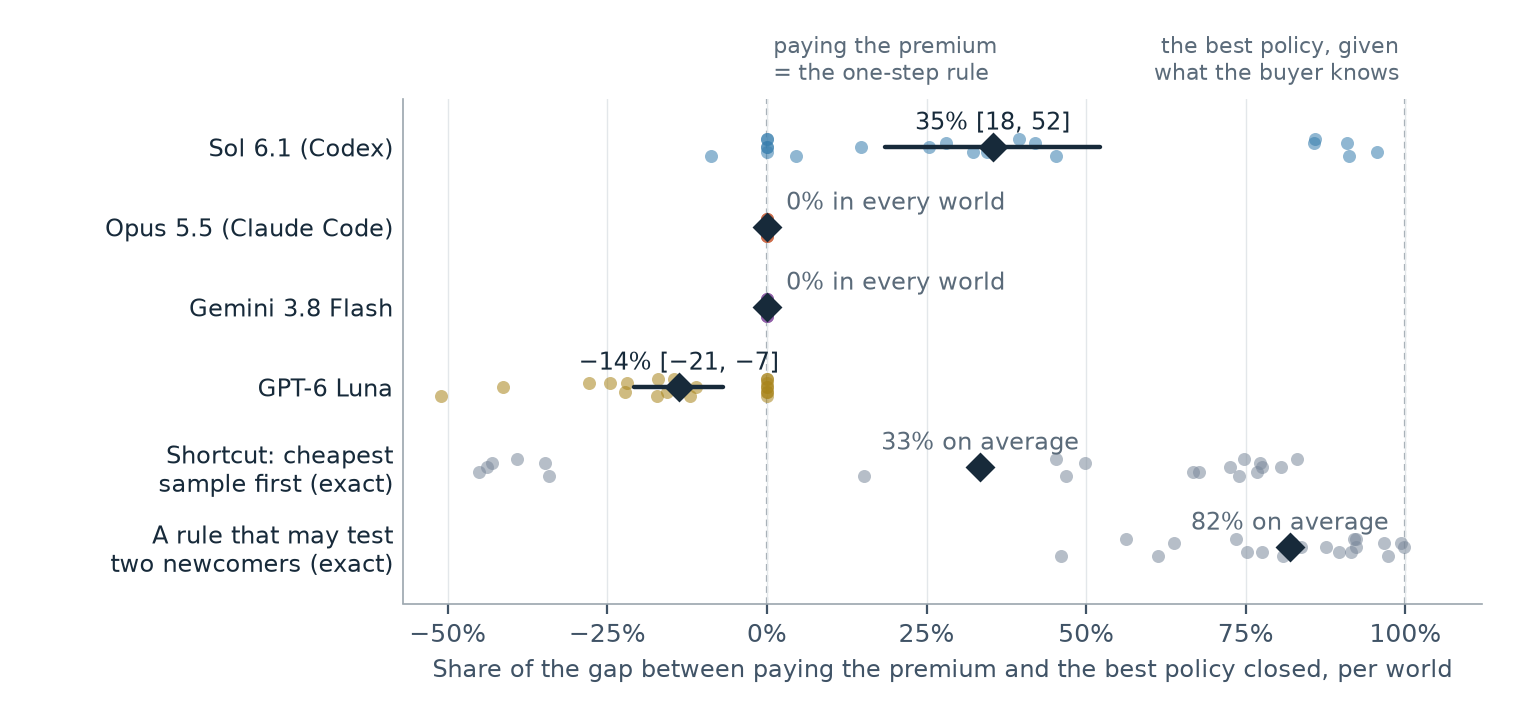
\includegraphics[width=\linewidth]{figures/procurement_v3_gap_closed.png}
\caption{\textbf{Procurement, the 20 pre-registered worlds: the share of the gap between paying the premium and the best policy closed, world by world.} Each dot is
one world, the mean of its two plays; diamonds are means and bars are 95\% t intervals. Paying the premium and a rule
that plans one newcomer's test exactly both sit at 0\% in every world. Opus and Gemini close none of the gap in any
world; Luna's orders of 50 units where 55 was best leave it below paying the premium. The gray rows are exact rules:
the shortcut that ignores seller kinds and first samples the newcomer whose sample is cheapest, and a rule allowed to
test two newcomers.}
\label{fig:5.1}
\end{figure}

Sol 6.1 closed 35\% of the gap (95\% t interval 18--52\%, p = 0.0003), whereas a rule that plans one newcomer's test
exactly closes none. This was the one test we pre-registered before any play, and the claim holds; it concerns Sol
alone. Its play varies by world (Figure 5.1): it closes most of the gap in some worlds and none in others. The other
three models never touched a newcomer. Opus 5.5 and Gemini 3.8 Flash paid the premium in every play; GPT-6 Luna did
too, but it ordered 50 units where 55 was best in 15 of its 40 plays, which leaves it below paying the premium. A
shortcut that ignores seller kinds and first samples the newcomer whose sample is cheapest closes 33\%, about Sol's
share, but Sol does not play that shortcut: it opens with the shortcut's move in 2 of 40 plays, and its tests follow
price. The moves the case is built around are rare in its play: it tests a second newcomer in 7 of 40 plays and looks
up a source in 4. A rule allowed to test two newcomers closes 82\%, so the remaining headroom lies in planning one test
beyond the one in hand.

Further runs on this evaluation set are reported in Appendix E.4 (Table E.15): a development pilot, the
pre-registered worlds at the earlier evaluation set's more favourable odds, and a task prompt corrected for four
wording defects. None of them changes this picture. One of them bears on why Opus never tests. In a check with no
play, Opus was asked how likely a newcomer is to be sound once another newcomer of its kind has passed or failed a
sample, with and without a clean quote of its own first, and it answered all 18 questions within 0.05 of the exact
value, as Sol did. Opus therefore applies the sharing rule correctly when asked, but does not plan with it. These runs
used the case's environment from a development branch, which is now on the main branch with its registration; every
published receipt replays through the runtime's command line (Appendix F.1). On an earlier evaluation set, in which
quotes always arrive and newcomers never share a source, performance saturates: a rule that looks one test ahead comes
within 0.01\% of the best policy (Appendix E.4, Table E.14).

\textbf{Data center.} The structure follows a real AI-infrastructure engagement in which a system integrator bundles
hardware, data-center space, staffing and software into a working system for a client. Hardware can arrive late or
defective, the site may not be ready, and the contract's warranty, delay-damages, liability-cap, site-readiness,
deposit and burn-in clauses decide who bears each cost. We set the costs, probabilities and prices ourselves. Client
and integrator negotiate one agreement, consisting of a position on each of the eight clauses (600 distinct
agreements) and an all-in price p.~Each side knows its own cost of carrying risk and only the probability distribution
of the other's: the integrator's pre-staging cost and risk charge, and the client's risk charge. Over six alternating
moves, a side may redline any clauses and name a price, sign the standing version, or walk away, and each redline
after the first move costs \$25k. In thousands of dollars and net of redline fees, a signed agreement c pays the
integrator and the client, respectively,

\[ \text{π\_I = p − C\_I(c) − 500,  π\_C = O\_C − p − C\_C(c),} \tag{3} \]

where 500 is the integrator's outside option, O\_C the client's, and C\_I and C\_C each side's expected cost of the risks
that the clauses leave with it, marked up by its risk charge; no deal pays only the fees. The difficulty is that price
only divides the value, while the clauses determine how much value there is, and the best clauses depend on what the
other side hides. Burn-in, for example, costs the integrator \$40k and, in one world, costs the client a week's delay
worth \$110k, and it halves the probability of a \$3 million incident that the client carries. It therefore lowers joint
cost by \$41k for a client with the highest risk charge and raises it by \$19k or \$64k for the other two, and the
integrator cannot tell which client it faces. The comparison reported here (v2) was pre-registered before its runs, on
80 included worlds (from 5,436 scanned), 72 of them with a mutually beneficial deal. Both command-line tools were
isolated, the client's task prompt states its walk-away point, and a world is included only if the integrator has at
least \$25k of room over a price-only rule. An earlier pre-registered comparison (v1) did none of these three things;
it is reported in Appendix E.4 (Table E.16), and development results remain in Tables E.3 and E.7.

\renewcommand{\thetable}{5.4}
\begin{longtable}[]{@{}
  >{\raggedright\arraybackslash}p{(\linewidth - 6\tabcolsep) * \real{0.2143}}
  >{\raggedleft\arraybackslash}p{(\linewidth - 6\tabcolsep) * \real{0.2857}}
  >{\raggedright\arraybackslash}p{(\linewidth - 6\tabcolsep) * \real{0.2143}}
  >{\raggedleft\arraybackslash}p{(\linewidth - 6\tabcolsep) * \real{0.2857}}@{}}
\caption{\textbf{Data center, the pre-registered comparison (v2): Sol 6.1 (Codex) and Opus 5.5 (Claude Code). Differences in a seat's earnings above its outside option, at true costs, on the 72 deal worlds, in percentage points of the value available in a deal (the joint surplus of the best agreement, \$309k a world); intervals are 95\%, with Holm correction across the four primary contrasts. Gate 3 passes for the integrator seat; Gates 0, 1, 2, 4 and 5 are partial (Table 6.1).}}\label{tab:5.4}\tabularnewline
\toprule\noalign{}
\begin{minipage}[b]{\linewidth}\raggedright
Primary contrast
\end{minipage} & \begin{minipage}[b]{\linewidth}\raggedleft
Worlds
\end{minipage} & \begin{minipage}[b]{\linewidth}\raggedright
Estimate {[}95\% interval{]}
\end{minipage} & \begin{minipage}[b]{\linewidth}\raggedleft
Holm p
\end{minipage} \\
\midrule\noalign{}
\endhead
\bottomrule\noalign{}
\endlastfoot
Head to head: Sol minus Opus earnings, seat-averaged & 72 deal & +41.7 {[}31.3, 52.0{]} & 6.1e-11 \\
Integrator against the firm client: Sol minus Opus & 72 deal & +7.5 {[}1.7, 13.2{]} & 0.022 \\
Sol as integrator minus the price-only rule & 72 deal & +7.3 {[}2.6, 12.0{]} & 0.008 \\
Opus as integrator minus the price-only rule & 72 deal & −0.2 {[}−5.5, 5.2{]} & 0.95 \\
\end{longtable}

All freeze and run probes were clean, and all 640 negotiations are valid and replayed (\$55.41 at list price). The
head-to-head gap is 41.7 points and the firm-client gap 7.5; each is detected under the Holm correction, and neither is
shown to reach its pre-registered minimum (32.4 and 12.9 points, \$100k and \$40k). Head to head, the opponent changes
with the focal model, whereas the firm-client contrast holds the counterpart policy fixed, which supports a
counterpart-specific reading of the larger gap. As integrator, Sol beats the price-only rule, and Opus earns what the
rule earns. With the walk-away point stated, neither model signs below it as client (0 of 80 for either), and the
client seat separates nothing (+0.8 points {[}−3.2, 4.9{]}).

We computed the best informed turn-by-turn policy after both runs, against the same scripted counterpart
(Appendix C.3). On v2's deal worlds it gives the integrator 63.5\% of the value available at the true client type,
whereas Sol earned 33.8\%, Opus 26.3\% and the price-only rule 26.5\%. Sol therefore captures about 20\% of the room
between the rule and that reference. In both seats and both campaigns, knowing the other side's type is worth less than
1\% of the value available to this policy, so the case measures bargaining against a fixed counterpart far more than
inference about it.

\subsection{Where the shortfall comes from}\label{where-the-shortfall-comes-from}

Figure 5.2 divides each case's shortfall into observed action classes. The components sum to the total under a stated
priority order, and they describe what happened, not its cause. Each panel uses its own reference and units.
Appendix E.5 gives the classification rules and the full subject tables, and Appendix E.7 gives the current Data-center
breakdown and its uncertainty. Table E.10 retains the exact panel values.

\begin{figure}[htbp]\centering\renewcommand{\thefigure}{5.2}
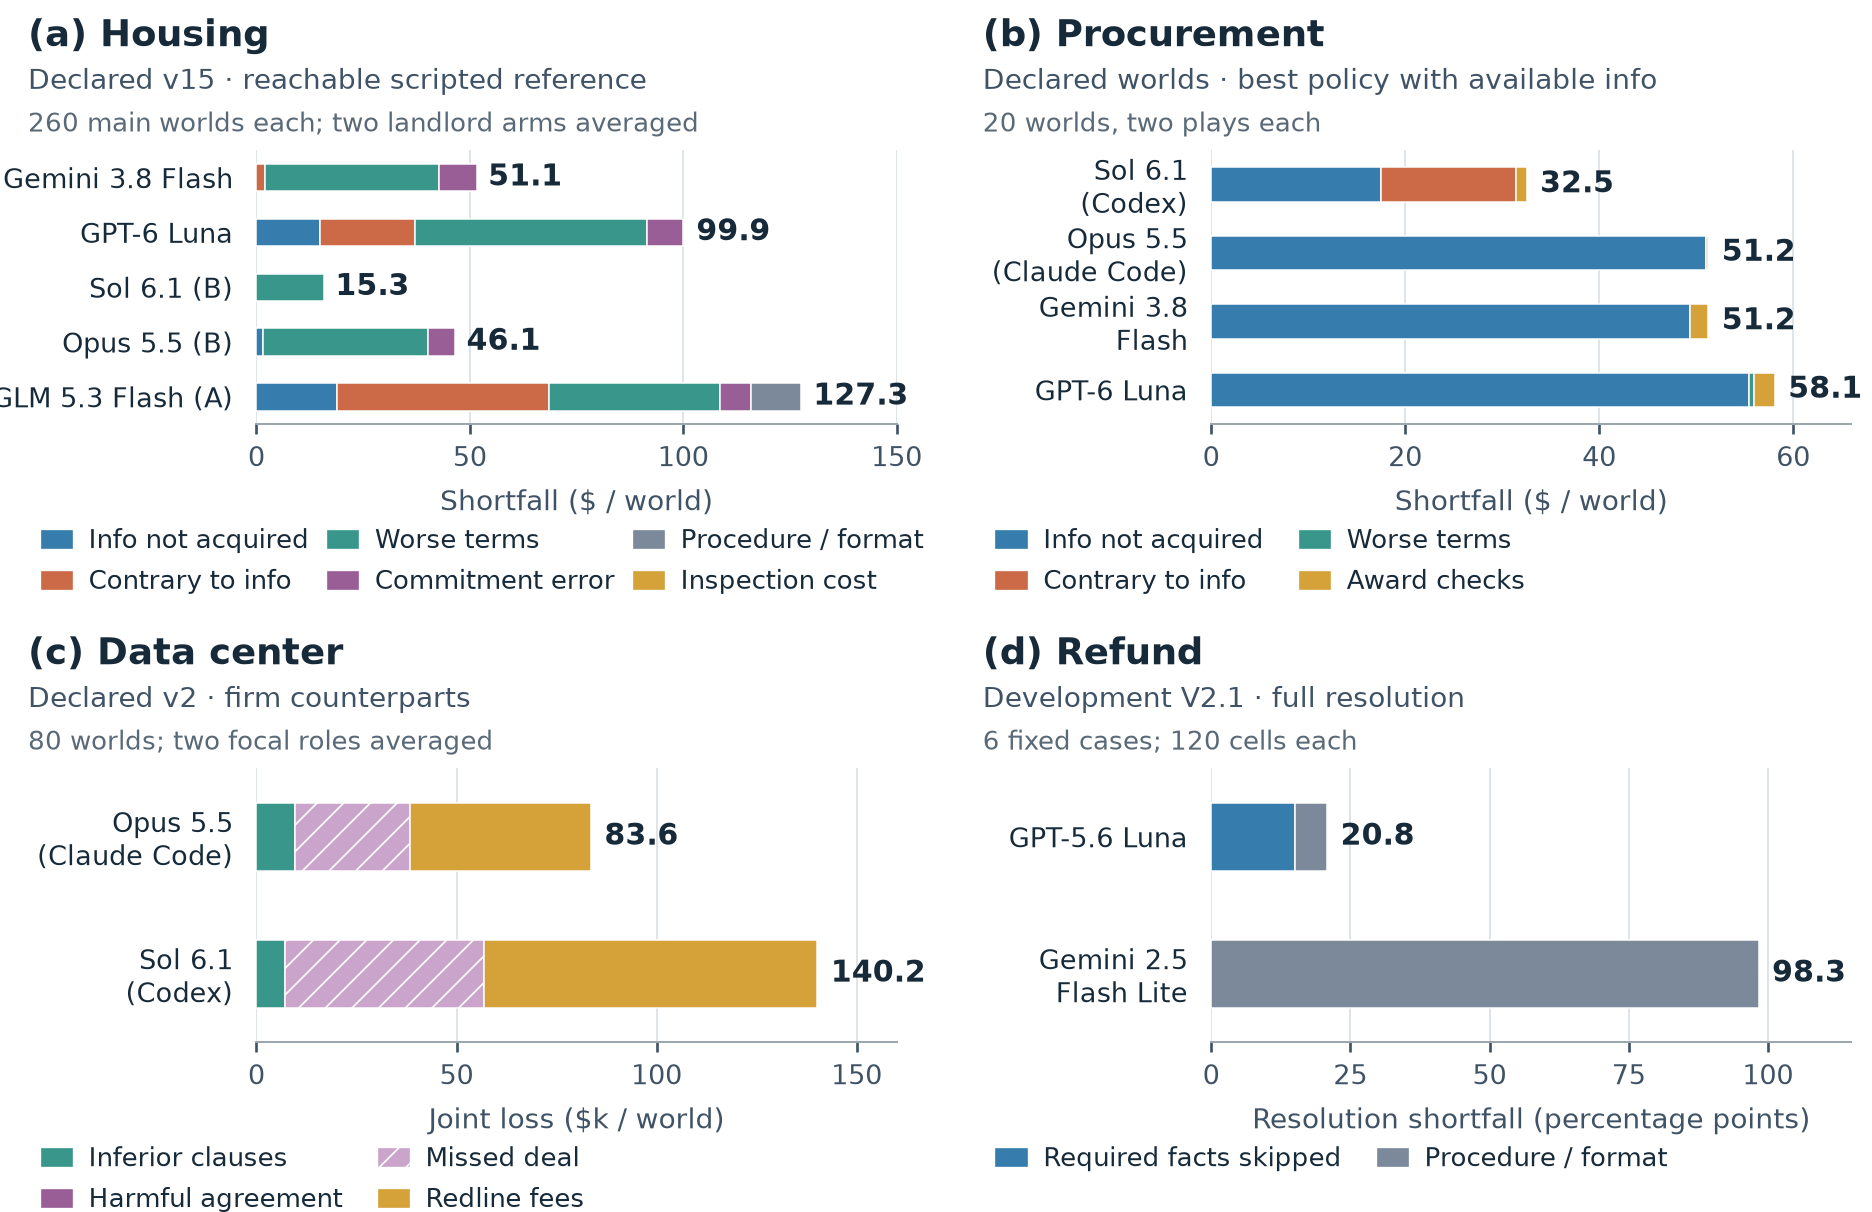
\includegraphics[width=\linewidth]{figures/shortfall_by_case.png}
\caption{\textbf{Shortfall to each case's reference.} Segments account for observed actions, and labels give mean totals
(lower is better within a panel). Units and scales differ across panels. Housing shows v15's two pre-registered models
and the three addendum subjects (A: GLM; B: Sol and Opus through their command-line tools) on the 260 main worlds of
Table 5.2, measured below the reachable scripted rule (\texttt{inspect\_\allowbreak{}lowball}, as in Table 5.2's fourth row); the few
negative amounts, at most \$0.4 a world, are in Table E.10 and are not drawn. Procurement shows all four subjects on
the 20 pre-registered worlds of Table 5.3; full subject tables are in Appendix E.5. Data center reports v2's joint loss
relative to the full-information bound with the firm counterparts at \$25k per paid redline, across all 80 worlds of
Table 5.4 with both seats averaged. In Procurement, \$6.33 a world of Luna's information-not-acquired segment is the
worse-quantity part of awards made before a worthwhile test; the pre-registered classification rules file such an
award's whole loss under that class (Table E.10). Intervals and exact values appear in Tables 5.3, E.9 and E.10.}
\label{fig:5.2}
\end{figure}

The labels name what happened. The mechanism behind each large segment is as follows.

\textbf{Procurement: three models never test, and Sol secures the recorded supplier first.} Opus, Gemini and Luna asked
no newcomer for anything in any of their 120 plays: they requested quotes and samples from the recorded supplier and
awarded it the order, so nearly all of their loss is information not acquired, and the rest is award checks, each of
which spends an action. Luna's further \$6.85 a world comes from ordering 50 units where 55 was best in 15 of its 40
plays; the pre-registered classes file most of it under information not acquired (Table E.10). Sol's loss divides by
world. Where it never tested a newcomer that the best policy would have tested, it lost \$17.5 a world. Where it did
test, it often first requested a quote and a sample from the recorded supplier, spending days and actions before the
newcomer test that the stated odds and clock made best (\$8.9 a world), or it awarded the order while a newcomer test
it had begun was still worth finishing (\$3.2).

\textbf{Housing, Gemini: it drops a known lemon even where the lemon is the better lease.} Worse terms account for 80\% of
its shortfall relative to the reachable rule (\$40.7 of \$51.1 a world), and nearly all of it comes from one move. Under
the landlord kind that prices a lemon from its own lower cost, a lemon's landlord counters about \$1,000 below a sound
listing's floor (\$995 to \$1,000 in these worlds), so a known lemon signed at that counter is worth what the listing
would be worth sound at a sound floor. This holds exactly in 187 of the 200 worlds whose favourite is a lemon, and
within \$5 in the rest. The rule inspects the favourite, finds the lemon, offers \$0 and signs the counter in all 200.
Gemini also inspected the favourite and found the lemon in all 200, but made an offer on it in only 4; in 172 episodes
it leased a sound listing that left it with less (\$65.0 a world). Under the other landlord kind the rule leases nothing
in 77 worlds, and Gemini's leases there offset \$26.5 a world. Gemini does read landlords' replies: of 74 replies that
proved a lemon, it walked away from 64 and signed above the lemon's value once. Ending with no lease where the rule
leased costs a further \$8.9 (12 of 520 episodes).

\textbf{Housing, Luna: it drops the lemons worth taking and signs ones that cost it.} Its shortfall relative to the
reachable rule is \$99.9 a world. Worse terms (54\%, \$54.3) follow Gemini's pattern: in the same 200 worlds Luna found
the lemon favourite in 197 and made an offer on it in 7, and in 154 episodes it leased a sound listing that left it
with less (\$57.7 a world). Signing a listing that a landlord's reply had proved a lemon accounts for 22\% (\$22.2,
11 episodes): the landlord accepted Luna's offer at a rent that no sound landlord would take, which by the stated
pricing rule proves a lemon, and Luna signed at that rent, above the lemon's value. Of 89 such replies, it walked away
from 58 and signed 20 at or below the lemon's value. Another 15\% (\$14.9, 64 episodes) comes from signing without
settling quality under the landlord kind whose replies reveal nothing, where an inspection was worth its \$25 fee every
time; 21 of those listings were lemons. Ending with no lease where the rule leased costs \$8.6. In v14, whose task
prompt did not state how landlords price, the reply-proved lemon accounted for 60\% of Luna's shortfall.

\textbf{Housing, Sol and Opus (addendum B): what remains is the price.} Neither lost anything by acting against what it
knew, and neither left a worthwhile inspection undone, apart from Opus's \$1.4 a world. Worse terms account for all of
Sol's \$15.3 shortfall (\$15.7, offset by \$0.4 of inspection fees it saved) and for 84\% of Opus's \$46.1 (\$38.8); ending
with no lease where the rule leased costs Opus a further \$6.3.

\textbf{Refund, Gemini 2.5 Flash Lite: the case ends before it decides.} In 81\% of its episodes it asked again for a fact
it had already been given; the environment rejects a repeated request, and the case ends with no decision (80.8 of its
98.3 points). In most of the remaining episodes it denied the claim correctly but wrote the refund method as null
where the policy's format requires ``none'' (16.7 points). It reached the answer key's outcome in 18\% of episodes and a
wrong outcome in none.

\textbf{Data center: fees, then deals the client walked away from.} Every redline after the opening move costs \$25k. The
full-information reference signs the best agreement at once, so each fee counts as loss, whichever side paid it.
Against the firm counterparts, across all 80 worlds with both seats averaged, fees account for 59\% of Sol's joint loss
(\$83.4k of \$140.2k a world) and 54\% of Opus's (\$45.3k of \$83.6k). Sol redlines more: as integrator it made 371
redlines to the firm client's 262, whereas Opus made 227 to 189. Some of those redlines buy better clauses, and a seat
that does not know the other side's costs may need them, so their share alone does not show wasted negotiation. Nearly
all of the remaining loss is deals lost in worlds that had one (35\% of Sol's loss and 34\% of Opus's), and every one of
them ended with the client walking away. With each model as integrator, the firm client walked away from Sol in 40 of
its 144 plays of deal worlds and from Opus in 14. As client, each model walked away in 26 of the 72 deal worlds. No
agreement was harmful: with the walk-away point in the task prompt, neither model signed in any of the 8 worlds
without a deal.

The pre-registered plan included a replay of the recorded moves at other fees, which shows what the same moves would
earn, not how the models would play. Without fees, Sol still loses more joint value than Opus against the firm
counterparts (\$63.1k against \$42.5k a world, seats averaged) and earns more in both seats. At \$50k a redline its
earnings fall below Opus's (as integrator 67.9 against 69.7, as client 1.3 against 22.8, in thousands of dollars per
deal world), because it redlines more. Appendix E.9 gives v1's fuller replay.

\textbf{Across the cases.} Four findings hold across the cases. First, the gap lies in a stratum that the design fixes in
advance, so every case reports by stratum and pools last. Second, the counterpart is part of the measurement, so a
claim names the counterparts it covers. Third, what the task prompt states moves the score as much as the subject does
(stating two rules cut procurement loss by \$11 to \$14; stating a walk-away cost cut losing signatures from 15 of 60 to
1 of 60), so the task prompt is a versioned part of the case. Fourth, a pattern found by looking back is a hypothesis
until a pre-registered test confirms it.

Housing, Procurement and Data center take their decision structure from real settings (Section 5.1): informal
rentals, wholesale sourcing and AI-infrastructure contracting. We set their parameters ourselves; they are not
calibrated to field data. The experiments use controlled scenarios and a small set of agent configurations, with no
human policy baseline, and they do not establish general model rankings.

\subsection{An external benchmark on the same runtime}\label{an-external-benchmark-on-the-same-runtime}

TERMS-Bench evaluates bilateral price negotiation against counterparts whose type is hidden \citep{zhang2026termsbench}. We reimplemented,
from the paper's description, its alternating-offer environment, three of its six counterpart families (Candid,
Taciturn and Expressive) and four of its measures as one AERead family. The counterpart runs as a scripted seat, and
its random draws are sealed each turn, so replay recomputes the counterpart's moves as well as the scores. We did not
implement the Oracle-Cue reference or the gap measures built on it, the urgency regime, type-belief error or the other
three families, and counterpart messages are templates. The corpus has 30 cases, 15 with a zone of agreement and 15
without, each played once.

\renewcommand{\thetable}{5.5}
\begin{longtable}[]{@{}
  >{\raggedright\arraybackslash}p{(\linewidth - 8\tabcolsep) * \real{0.1579}}
  >{\raggedleft\arraybackslash}p{(\linewidth - 8\tabcolsep) * \real{0.2105}}
  >{\raggedleft\arraybackslash}p{(\linewidth - 8\tabcolsep) * \real{0.2105}}
  >{\raggedleft\arraybackslash}p{(\linewidth - 8\tabcolsep) * \real{0.2105}}
  >{\raggedleft\arraybackslash}p{(\linewidth - 8\tabcolsep) * \real{0.2105}}@{}}
\caption{\textbf{TERMS-Bench reimplementation: two of the paper's agents on the same 30 cases, scripted
counterpart and settings. Agreement and surplus are computed over the cases with a zone of agreement: 15 for
GPT-4o-mini and 12 for GLM-5.1, whose three malformed moves removed those episodes. Paper values:
surplus efficiency from its Table 16 (overlap regime, mean of the three families played here);
agreement and conditional surplus efficiency from its Table 2, which pools six families and three
regimes.}}\label{tab:5.5}\tabularnewline
\toprule\noalign{}
\begin{minipage}[b]{\linewidth}\raggedright
\end{minipage} & \begin{minipage}[b]{\linewidth}\raggedleft
GPT-4o-mini
\end{minipage} & \begin{minipage}[b]{\linewidth}\raggedleft
GLM-5.1
\end{minipage} & \begin{minipage}[b]{\linewidth}\raggedleft
Paper: GPT-4o-mini
\end{minipage} & \begin{minipage}[b]{\linewidth}\raggedleft
Paper: GLM-5.1
\end{minipage} \\
\midrule\noalign{}
\endhead
\bottomrule\noalign{}
\endlastfoot
Agreement rate where a deal exists (AGR+) & 0.80 & 1.00 & 0.522 & 0.951 \\
Surplus efficiency (SE+) & 0.035 & 0.458 & 0.196 & 0.668 \\
Conditional surplus efficiency (CSE+) & 0.044 & 0.458 & 0.363 & 0.721 \\
\end{longtable}

The reimplementation orders the two agents as the paper does on all three measures, but absolute levels are lower for
both, and for a third model. A review of the port after these runs traced the shift to four departures from the
paper's protocol rather than to the agent, whose interface in the paper is also one stateless call per round. First,
our prompt does not state the agent's payoff or the rule against accepting above its reservation value. Second, its
observation differs from the paper's. Third, a malformed move removes the episode where the paper applies a fallback;
under that fallback, GLM-5.1's surplus efficiency would be 0.520 over all 15 cases. Fourth, our price range and zone
widths are wider than the paper's. We have built a pre-registered reproduction with those fixes, and it stopped at its
first check: one of the paper's fixed-concession baselines (FC10) scores 0.307 here against the paper's 0.266, while
the other two match. The paper states how much the baselines concede (1\%, 10\% or 30\% of the remaining distance per
offer) but not how they open or accept. No agent has played the reproduction. The paper reports critical violations
by GLM-5.1 in 5\% of cases without a zone of agreement for these three families; at that rate, 15 such cases would show
none about half the time, and ours showed none. The port also exposed a harness effect. On one provider route, any
specified reasoning budget suppressed deliberation, and GLM 5.3 Flash breached its own reservation value in 13 of
30 cases, against the paper's band of 0 to 2.06\%. With no reasoning setting specified, it breached in 2 of 30 and its
surplus efficiency rose from 0.40 to 0.53; the comparison above uses that setting. This is why the reasoning condition
is part of each run's frozen configuration. The runtime's support for the scripted seat that this family uses is now
on the main branch.

\section{Quality control}\label{quality-control}\label{sec:qc}

The defects that mattered in the four cases were properties of the distribution, the brief, the
counterpart or the analysis, and every world was individually correct when they were found: a
seat-number tie-break that decided who signed the good listing, a prompt that pointed
every subject at the right supplier in half the worlds and the wrong one in the other half,
a hidden type tied to the pack cell so that comparisons by type compared worlds.
Reading one world at a time passes all three. Quality control is therefore organised
around populations of worlds, declared analyses and recorded failures. Appendix F describes each
check that was applied to these cases, and only those.

\textbf{Gates.} A case is qualified in six gates recorded in its family's QC profile: a profile exists
(0); the worlds are valid, distinct, split and leave headroom (1); actions change the intended
state and every score is rebuilt from sealed evidence (2); a better-informed policy does better
and shortcuts lose (3); the result supports the attribution it claims (4); and the comparison was
sized, frozen and executed without tuning on outcomes (5). Each gate is typed \texttt{passed}, \texttt{failed},
\texttt{partial}, \texttt{not\_run} or \texttt{not\_\allowbreak{}applicable}, and only \texttt{passed} promotes. The profiles followed the initial
runs; the agreement confirmatory followed its profile. None passes Gates 1 to 5 yet (Table 6.1).

\textbf{Table 6.1. Gate status of each reported comparison,} from its family's QC profile on 21 October. A gate's flags are
what its checks found without blocking it; they qualify the claim.

\begin{longtable}[]{@{}
  >{\raggedright\arraybackslash}p{(\linewidth - 6\tabcolsep) * \real{0.2500}}
  >{\raggedright\arraybackslash}p{(\linewidth - 6\tabcolsep) * \real{0.2500}}
  >{\raggedright\arraybackslash}p{(\linewidth - 6\tabcolsep) * \real{0.2500}}
  >{\raggedright\arraybackslash}p{(\linewidth - 6\tabcolsep) * \real{0.2500}}@{}}
\toprule\noalign{}
\begin{minipage}[b]{\linewidth}\raggedright
Comparison
\end{minipage} & \begin{minipage}[b]{\linewidth}\raggedright
Passed
\end{minipage} & \begin{minipage}[b]{\linewidth}\raggedright
Not passed, and why
\end{minipage} & \begin{minipage}[b]{\linewidth}\raggedright
Flags
\end{minipage} \\
\midrule\noalign{}
\endhead
\bottomrule\noalign{}
\endlastfoot
Housing v15 (Table 5.2) & 0, 1, 2, 3, 5 & 4 \texttt{partial}: the declared one-call profile probe ran only after the freeze & \texttt{inspect\_\allowbreak{}lowball}, which inspects the favourite, offers \$0 and signs the counter when the inspected value covers it, comes within \$25 of the best informed tenant in 229 of 260 worlds and equals it in all 60 with a sound favourite; every shortcut loses at least \$25 in every world \\
Procurement, declared pack (Table 5.3) & 0, 1, 2, 3, 5 & 4 \texttt{partial}: the command-line subjects take no seed, and the runtime registration merged on the owner's override & looking two newcomers ahead loses \$8.38 a world, as little as \$0.09; Opus's and Gemini's two plays of a world always scored the same, Sol's in 7 of 20 worlds \\
Data-center agreement v2 (Table 5.4) & 3, integrator seat & 0, 2, 5 \texttt{partial}: its registry row awaits a non-author review and its code is not on the main branch, so replay through the runtime's command line has not run; 1 \texttt{partial}: its grid reference is a lower bound, so only the control route applies and it has not run; scored against that reference, a shortcut comes within 25 in 12 of 80 worlds, all 8 where no deal is possible (walking earns the reference, and every scripted rule walks) and 4 of 72 deal worlds; the client seat keeps its construct limit; 4 \texttt{partial}: the command-line subjects take no seed & a model's two plays of a world ended identically in 47 of 80 worlds for Opus and 28 for Codex; some fixed negotiating style comes within 25 of the reference in 27 of the 72 deal worlds \\
Refund V2.5 (developmental) & 0 & 3 \texttt{failed}: a full refund that collects no fact is fully right on 38 of 180 policy cases, and naive controls come close to the reference in three of four seats; 1, 2 and 4 \texttt{partial}; 5 not run & no model has played it \\
\end{longtable}

\textbf{Headroom (Gate 1) is shown in one of two ways.} Where a case computes its reference exactly, as Housing and Procurement
do, its profile names the shortcuts, rules that skip the decision the case measures, and every
shortcut must lose a declared margin to the reference in every admitted world; rules that do make the decision are
reported beside it, as the flags above are. Where the reference is estimated, a frozen model control is played on the
worlds before they are frozen; the agreement's grid reference is a lower bound, so it needs that route, which has not
run. The first way was added on 21 October, after Procurement's frozen control proved weaker
than the shortcuts it was compared with, so the check measured the control rather than the worlds (Appendix F.1).

\textbf{The reference is played on every world.} For each case a test plays the reference through the
real environment and verifier on every admitted world, with no model, and checks that it reaches
its declared result: the Housing reference and a full-information tenant reproduce the published
values in all 600 v14 cells, and the full-information tenant reaches the ceiling on all 320 v15 worlds; on Procurement's harder pack the best policy and the one-step rule equal their averages over 400
plays through the environment, within four standard errors, on all 12 pilot worlds and all 20 worlds of the declared
test (the declared worlds checked on 20 October, after the runs), and on the
earlier pack the best policy equals the environment's average over its 27 type profiles in all 24 worlds; the data-center oracle pair loses nothing in all 116 worlds of
both development packs, all 60 of v1's admitted pack and all 80 of v2's (checked on 20 October, after its runs); Refund V2.5's release requires full credit on every case. The initial tests followed development; the admitted-pack dry run preceded the confirmatory; two of them (the data-center grade and the Housing ceiling) are shown to fail when the grade
or the reference is wrong.

\textbf{Other checks.} Every committed pack is regenerated byte for byte from its seeds; the Housing
v14 and v15 receipts replay from their sealed events; trivial agents are reported beside the subjects,
Procurement's fixed rules are scored exactly, and the briefs were audited for instructions that
decide the outcome. Uncertainty is computed over worlds, claims name their counterparts, and five
reported analyses were declared before their runs: Housing v14 and v15, the data-center signalling
test and the two agreement confirmatories.

\textbf{What it found.} Discovered failures are recorded in an incident log in design,
operational, tooling and judgment rows that are never deleted (51, 57, 90 and 23 distinct entries across
the project's logs). Of 25 defects selected for Table F.4, 14 were invisible in any single
world; the 11 visible ones were found by reading code or sealed bytes, by tracing a case, or in a
single gate cell (Table F.4). Nine were open when the table was compiled; a later reanalysis from the sealed actions resolves
one of them for the reported panels, leaving eight open. The same checks corrected three of our own
statements while this paper was written.

\section{Discussion and conclusion}
\label{sec:discussion}

\subsection{What the cases show}
\label{sec:discussion-findings}

AERead evaluates an agent's economic decisions by the value it obtains for
a principal, given the information, resources and authority of its seat.
Each score is measured against a reference whose access to information is
stated, whether a feasible policy, the best policy under the seat's
information or a full-information bound, and it keeps its own units and
names the counterparts it was measured against, so that every shortfall
has a defined interpretation. The worked examples apply this to
information acquisition, bargaining and commitment in housing, procurement
and contracting, and a reimplementation of part of TERMS-Bench runs on the
same runtime.

The cases teach three lessons that bear on any evaluation of this kind.
The counterpart is part of the measurement: the same two agents differ by
far more when they negotiate with each other than when each faces a fixed
counterpart. The brief is part of the case: stating a rule it had left
implicit moved scores as much as changing the agent did. And the defects
that matter are often properties of the population of worlds, the brief or
the analysis rather than of any single world, which is why construction
and quality control belong in the method; the checks of Section 6 changed
the interpretation of our own results. Loss categories locate a shortfall
but do not explain it, and explaining it requires controlled follow-up
comparisons. Replay establishes consistency with recorded play; construct
validity requires evidence about the worlds, the information and the
controls.

These properties matter most where agents are deployed. Organizations that
pilot agents often stop because the business value is unclear and the
risks are hard to control \citep{gartner2025agentic}; a value score against
a stated reference and a typed account of losses address both. Small firms
face a different problem: short of staff \citep{nfib2026jobs}, they often
leave decisions like those our cases model to one person, without
specialized expertise and with no review before a commitment. Delegating
such a decision to an agent is attractive there, and trusting it requires
evidence that the agent keeps value against the counterparts it will meet.

The present evidence has clear limits. The cases take their decision
structure from informal rentals, wholesale sourcing and AI-infrastructure
contracting, but their parameters are set by the authors; calibration to
field data and transfer to field settings remain to be established.
Coverage is limited to two transaction classes and a small set of agent
configurations, with no human policy baseline. Housing v15 and Procurement's
declared pack pass four of the five qualification gates and no case passes
all five: several checks were added after the runs they qualify, and hosted-model and CLI
behavior limits attribution from declared settings.
Versioned reanalyses now regenerate the corrected Housing measures and
Procurement decision losses from sealed records, which strengthens their
provenance, but full verification against original execution still
requires retained logs (Appendix~G), and the reanalyses neither qualify the
campaigns retroactively nor resolve Housing's historical seat attribution
(Appendix~H). The results therefore compare named agents on stated worlds;
they do not establish general model rankings or deployment readiness.

\subsection{Open research directions and contributions}
\label{sec:open-directions}

AERead is shared infrastructure for studying how agents make economic
decisions. Its code is open source under the Apache-2.0 license
(github.com/aeread-org/AERead; contact@aeread.org), and contributors can
pursue their own questions with the existing cases, counterparts and
evidence. The results above leave four questions open, each suited to a
different kind of contribution.
\begin{itemize}
\item \textbf{Counterpart populations.} The Data-center gap between two
agents is 42\% of the value available in a deal head to head and 7\%
against a fixed script.
How far does an agent's measured skill depend on whom it faces, can
rankings reverse across counterpart populations (none did in our runs),
and which populations separate distinct strategic capabilities? The
scripted styles, head-to-head pairings and counterpart seats are in place.
\item \textbf{Validity of populations of worlds.} Of 25 defects selected
from our record, 14 were invisible in any single world. Which checks find
such defects before a campaign runs, and what should qualify a case? The
quality-control gates, the incident record and the failed campaigns are
available for study.
\item \textbf{Information and judgment.} Stating a rule the brief had left
implicit moved scores as much as changing the agent. Separating what an
agent was told from how it decided, and computing best-informed references
for richer cases, are open methodological problems.
\item \textbf{New economic decisions.} A case for another activity
supplies its rules, worlds and reference; execution, replay, counterpart
seats and the quality-control standard come with the runtime.
\end{itemize}

What is ready and what is not: the runtime, its sealed evidence and
replay, and the case layout are in use, and Housing, Procurement and Data
center each have a world generator, references and scripted counterparts.
No case is yet fully qualified: Housing v15 and Procurement's declared pack
pass four of the five gates.
Section~\ref{sec:qc} gives every gate verdict and
Appendix~F each campaign's open checks, so a contributor can see what a
case still needs before its results can rank agents.

The next steps follow from the limits in Section 7.1. Future campaigns should bind
actual seat assignments and headline scorers into frozen evaluation
identities and run the required controls before any comparison, and the
TERMS-Bench reimplementation needs the protocol fixes described in
Section 5.3 before a declared reproduction. Practitioner review would
calibrate the cases' parameters, human baselines would show where agents
stand against people, and externally contributed cases would test whether
the structure serves authors other than its maintainers. AERead's present
contribution is that structure, a common way to construct evaluations of
economic decisions, together with an evidence-based account of the checks
needed to interpret what they measure.


\bibliographystyle{plainnat}
\bibliography{runtime}

\appendix
\section{Case specifications}\label{case-specifications}

Following TERMS-Bench \citep{zhang2026termsbench}, we write each case as an environment Γ (outcomes, private types and their prior,
payoffs), a protocol (seats, order of play, actions, what each seat observes, termination), and fixed
counterpart policies (Appendix B). We do not specify Refund here. Symbols are local to each case, and each case's
table lists them together with the kind of quantity each one is. The subscript A denotes the evaluated seat and B a
counterpart. In controlled comparisons, the prior and the counterpart policies are fixed across evaluated agents;
head-to-head role swaps change the opponent as well, so they compare pairings rather than agents. Agent
configurations also differ in the settings recorded in Appendix H. We compute the reference policies of Appendix C
in the same Γ.

\textbf{Notation used across cases.} 𝟙{[}·{]} (or 𝟙(·)) is 1 when the condition inside holds and 0 otherwise. U(a, b) is a
uniform draw between a and b. 𝔼 is an expectation over the outcomes the case lists, and ⌊x⌋ rounds x down. D denotes
each case's loss: the lemon loss (\$1,000) in Housing and the value of supplying nothing (−\$600) in Procurement.
Each case's table defines its other symbols, and Appendices C and D refer back to it when they reuse one.

\textbf{Terms used across the cases.} A \emph{world} is one fully specified environment instance of a case, that is, its
parameters and hidden types, fixed by a seed. An evaluation set is a published set of worlds that can be
regenerated from their seeds, and its inclusion criterion, computed before any agent plays, decides which generated
worlds enter it. A \emph{seat} is a player position (the tenant, a landlord, the buyer, the integrator); the evaluated
agent holds one seat, and scripted policies or other agents hold the rest. An episode is one play of one world
under one condition (in Housing, one world and one landlord kind). A frozen configuration (such as v14 or v15) fixes
an evaluation set, a task prompt, the counterparts and the controls; changing any of them creates a new
configuration. A comparison is pre-registered when its plan and analysis were committed to the repository before any
of its episodes ran. A \emph{reference} is the policy or bound against which a case measures a shortfall, with its access
to information stated (Appendix C). A \emph{gate} is one of the six quality-control gates of Section 6, numbered 0 to 5:
a check that a result must pass before it is reported as qualified.

\subsection{Housing: lemons with outside demand (frozen configurations v14 and v15)}\label{housing-lemons-with-outside-demand-frozen-configurations-v14-and-v15}

The v15 configuration uses the same rules as v14. Its task prompt states the landlords' pricing rule, its worlds come
from a screened evaluation set (Appendix E.2), and its holdout sets the outside-demand rate to 0.3 a round.

\textbf{Environment.} A world seed w fixes four listings ℓ ∈ \{0, 1, 2, 3\} and six tenant seats.
Seat 0 is the evaluated tenant, seat i ∈ \{1, \ldots, 4\} is the outside demand for listing i − 1, and seat 5
never acts. Exactly m = 2 listings are lemons, Λ ⊂ \{0, \ldots, 3\}, drawn uniformly from a random
stream separate from the one that sets values, asks and costs. Seat 0 signs at most one lease
(ℓ, rent), or none. Its payoff after signing ℓ with k inspections is

\[ \parbox{0.86\linewidth}{\raggedright u\_A = v\_ℓ − D·𝟙[ℓ ∈ Λ] − rent − c·k, and u\_A = −c·k if it signs nothing,} \tag{A.1} \]

where D is the lemon loss and c the inspection fee (Table A.1).

Seat 0 privately knows v\_ℓ, its value for each listing if the listing is sound. Each landlord privately knows
its listing's quality and cost. The prior is uniform over the six possible lemon pairs. The
landlord kind is not drawn: both kinds are played on every world.

Every landlord has a target rent: it accepts any offer at or above the target and answers a lower offer with a
counter at the target (Appendix B.1). The two kinds differ only in where the target comes from. A \emph{leaky} landlord
prices off its own cost. A lemon costs its landlord \$1,000 less, so a lemon's landlord will rent for about \$1,000
less than a sound listing's landlord, and an offer between the two rents is accepted only by a lemon's landlord: the
acceptance itself shows that the listing is a lemon. A \emph{pooled} landlord prices every listing as if it were sound, so
its replies carry no information about quality. Each world is played once under each kind.

\renewcommand{\thetable}{A.1}
\begin{longtable}[]{@{}
  >{\raggedright\arraybackslash}p{(\linewidth - 4\tabcolsep) * \real{0.3333}}
  >{\raggedright\arraybackslash}p{(\linewidth - 4\tabcolsep) * \real{0.3333}}
  >{\raggedright\arraybackslash}p{(\linewidth - 4\tabcolsep) * \real{0.3333}}@{}}
\caption{\textbf{Housing parameters.}}\label{tab:A.1}\tabularnewline
\toprule\noalign{}
\begin{minipage}[b]{\linewidth}\raggedright
Symbol
\end{minipage} & \begin{minipage}[b]{\linewidth}\raggedright
Meaning
\end{minipage} & \begin{minipage}[b]{\linewidth}\raggedright
Value
\end{minipage} \\
\midrule\noalign{}
\endhead
\bottomrule\noalign{}
\endlastfoot
T & rounds & 3 \\
m & lemons & 2 of 4 \\
D & lemon loss (cuts the tenant's value and the landlord's cost alike) & \$1,000 \\
c & inspection fee & \$25 \\
a\_ℓ & ask & ⌊U(1500, 3200)⌋ \\
v\_ℓ & seat 0's value if sound & a\_ℓ + 10·s\_ℓ + U(−20, 20), with s\_ℓ = 100(0.6κ\_ℓ + 0.4ι\_ℓ) − 30 and κ, ι \textasciitilde{} U(0, 1); κ\_ℓ and ι\_ℓ are listing attributes shown on the board, which move seat 0's value but say nothing about quality \\
c\^{}S\_ℓ & a sound listing's cost & max(0, a\_ℓ − U(20, 80)) \\
c\^{}L\_ℓ & a lemon's cost & max(0, c\^{}S\_ℓ − 1000) \\
μ & landlord margin: a landlord's target is its reservation plus μ, capped at the ask (B.1) & \$25 \\
β & outside-demand rate per round & ½ (v15's holdout: 0.3) \\
\end{longtable}

In the main evaluation set, asks range from \$1,501 to \$3,198, and seat 0's gain v − a ranges from −\$275 to +\$676.

\textbf{Protocol.} Each round r = 0, 1, 2 has four phases. (1) \emph{Inspect}: seat 0 may pay c to
inspect one open listing it has not yet inspected, and the quality appears in its observation at once.
(2) \emph{Contact}: seat 0 makes one offer (ℓ, x) with ℓ open and x ≥ 0, or passes; offering again on
a listing it walked away from is legal. (3) \emph{Respond}: each landlord applies its policy (Appendix B.1) to its
inbox, and each listing creates at most one binding hold. (4) \emph{Commit}: a seat holding a hold signs
or walks; a missing or invalid action counts as a walk, and every hold expires at the end of the phase.
Signing ends seat 0's play, and the market ends after round 2 or when every listing is leased.

\textbf{Observation of seat 0.} Seat 0 observes the board (asks, uninformative listing attributes, and whether each
listing is open or leased), its rejected listings and active hold, its values v, the lemon count and share, the
loss, the fee, its own inspections and spending, and a history field (\texttt{your\_\allowbreak{}history}) that lists its own offers,
each hold with the binding rent and whether the landlord accepted or countered, and each sign or walk. The sealed
prompt states the payoff, that a fixed landlord ``may accept or make one binding counteroffer'',
that ``a counteroffer can itself convey information about listing quality'', the departure rule,
that a listing seat 0 bid on is protected in that round, the three-round horizon, that walking does
not close a listing, and the order of the phases. The v14 prompt states neither the landlord's pricing
rule nor the cost range. The v15 task prompt states both: a sound landlord accepts any offer at or above its cost
plus \$25 (or the ask, if lower) and otherwise counters at that amount, and since a sound listing's cost is \$20 to \$80
below its ask, a rent more than \$55 below the ask proves a lemon.

\textbf{Example: a reply and a signing.} A listing asks a = \$2,400. Its sound cost is c\^{}S = \$2,350, so
a lemon's cost is c\^{}L = \$1,350, and seat 0 values the listing at v = \$2,600 if sound. With the \$25 margin
(Appendix B.1), a sound listing's landlord targets \$2,375, a lemon's leaky landlord \$1,375, and a lemon's
pooled landlord \$2,375. Suppose seat 0 offers \$2,000. A sound landlord counters at \$2,375, and a pooled lemon
landlord also counters at \$2,375; a leaky lemon landlord accepts at \$2,000, and only a lemon's
landlord would, so the acceptance itself identifies the lemon. Signing pays v − rent = +\$225 for the
sound listing at \$2,375, v − D − rent = −\$400 for the leaky lemon at \$2,000, and −\$775 for the
pooled lemon at \$2,375. Inspecting first costs \$25 and reveals the quality under either kind. Had
seat 0 offered \$0, the leaky lemon landlord would have countered at \$1,375, which also identifies the
lemon, and signing at that rent pays +\$225.

\subsection{Procurement: pay or test (the earlier evaluation set)}\label{procurement-pay-or-test-the-earlier-evaluation-set}

\textbf{Environment.} One buyer sources one component. The suppliers are one recorded supplier E (an established
supplier with a sales record) and three newcomers N₁--N₃. Each supplier has a type θ ∈ \{G, L, P\} = \{(on-time 0.97,
yield 0.97), (0.55, 0.97), (0.97, 0.55)\}, that is, good, late or poor-yield; E is always of type G. Newcomer types
are independent. Newcomer i's prior is read from the cohort record of its seller kind, in which a\textsubscript{i} of 40 tracked
sellers were unreliable on delivery and b\textsubscript{i} failed inspection:

\[ \text{π\textsubscript{i} = (γ\textsubscript{i}, λ\textsubscript{i}, ρ\textsubscript{i}) = ((40 − a\textsubscript{i} − b\textsubscript{i})/40, a\textsubscript{i}/40, b\textsubscript{i}/40).} \tag{A.2} \]

The three newcomers therefore have 3³ = 27 type profiles, each with positive probability, and γ ranges from 0.2
to 0.7.

\renewcommand{\thetable}{A.2}
\begin{longtable}[]{@{}
  >{\raggedright\arraybackslash}p{(\linewidth - 2\tabcolsep) * \real{0.5000}}
  >{\raggedright\arraybackslash}p{(\linewidth - 2\tabcolsep) * \real{0.5000}}@{}}
\caption{\textbf{Procurement parameters.}}\label{tab:A.2}\tabularnewline
\toprule\noalign{}
\begin{minipage}[b]{\linewidth}\raggedright
Quantity
\end{minipage} & \begin{minipage}[b]{\linewidth}\raggedright
Value
\end{minipage} \\
\midrule\noalign{}
\endhead
\bottomrule\noalign{}
\endlastfoot
Kits owed / minimum service & 50 / 40 (an award completing fewer than 40 is void) \\
Revenue per kit / shortfall penalty & \$37 / \$12 per kit short \\
Supplying nothing, D & −\$600 (= −12·50), plus any information already spent \\
Cash budget & \$2,500 (never binds) \\
Deadline T & 10--12 days (clock ``none''), 13--14 (tight), 17--18 (loose) \\
Action budget & 10 \\
Order sizes & 50, 55 or 60 units (minimum order quantity, MOQ, 50; step 5; capacity 60); shipping \$0.60 a unit \\
E & price U{[}24, 28{]} rounded to \$0.05; lead 6 days; sample \$30 and 2 days; a record of 48--96 orders, 3\% late, 3\% defective \\
Newcomer i & price p\_E(1 − δ\textsubscript{i}), δ drawn without replacement from \{3, 5, 7, 9, 12, 15, 18, 21\}\%; lead 6--8 days; sample \$30--80 in \$10 steps and 3 days \\
Cohort record & a\textsubscript{i} ∈ \{4, 8\}, b\textsubscript{i} ∈ \{8, 14, 20, 24\} of 40 \\
\end{longtable}

\textbf{Payoff.} An award of q units at price p from a supplier with yield y, on-time rate r and lead time ℓ, made on
day t after spending I on information, is worth

\[ \parbox{0.86\linewidth}{\raggedright M = 37·k − 12·(50 − k) − C if k ≥ 40 and the order is valid, and M = D − I otherwise,} \tag{A.3} \]

where the number of kits completed is

\[ \parbox{0.86\linewidth}{\raggedright k = min(⌊q·y·r⌋, 50) if the order arrives by the deadline (t + ℓ ≤ T), and k = 0 if it arrives late,} \tag{A.4} \]

and the cost C is the sum of the terms in the following table:

\begin{longtable}[]{@{}
  >{\raggedright\arraybackslash}p{(\linewidth - 2\tabcolsep) * \real{0.5000}}
  >{\raggedright\arraybackslash}p{(\linewidth - 2\tabcolsep) * \real{0.5000}}@{}}
\toprule\noalign{}
\begin{minipage}[b]{\linewidth}\raggedright
Term of C
\end{minipage} & \begin{minipage}[b]{\linewidth}\raggedright
What it is
\end{minipage} \\
\midrule\noalign{}
\endhead
\bottomrule\noalign{}
\endlastfoot
q·p & the purchase \\
+ 0.6·q & shipping, \$0.60 a unit \\
+ q·p·0.12·15/365 & financing the purchase at 12\% a year for 15 days: the 45-day working-capital horizon less the 30-day payment terms \\
− R & the expected refund on defective units \\
+ R·0.12·10/365 & financing the refund, which arrives 10 days after the claim \\
+ I & the information bought \\
\end{longtable}

Here R is the expected refund on defective units: of the q·(1 − y) defective units, 90\% of claims are accepted and
refunded at the unit price, so

\[ \text{R = 0.9·q·(1 − y)·p.} \tag{A.5} \]

For a good supplier, an order of q = 55 units is optimal at every price in the evaluation set, and before
information costs the award is worth

\[ \text{A(p) = 1817 − 53.79p.} \tag{A.6} \]

With 55 units at y = r = 0.97 all 50 kits are completed, so 1817 = 37·50 − 0.6·55 and
53.79 = 55(1 + 0.12·15/365) − 1.485(1 − 0.12·10/365), where 1.485p = 0.9·55·0.03·p is the expected recovery on
defective units.

\textbf{Protocol.} The buyer takes one action at a time until it takes a terminal action (an award or a deferral,
Table A.3), exhausts the action budget, or takes an invalid action. A deferral, an exhausted budget and an invalid
action are each worth D − I.

\renewcommand{\thetable}{A.3}
\begin{longtable}[]{@{}
  >{\raggedright\arraybackslash}p{(\linewidth - 4\tabcolsep) * \real{0.3333}}
  >{\raggedright\arraybackslash}p{(\linewidth - 4\tabcolsep) * \real{0.3333}}
  >{\raggedright\arraybackslash}p{(\linewidth - 4\tabcolsep) * \real{0.3333}}@{}}
\caption{\textbf{Procurement actions.}}\label{tab:A.3}\tabularnewline
\toprule\noalign{}
\begin{minipage}[b]{\linewidth}\raggedright
Action
\end{minipage} & \begin{minipage}[b]{\linewidth}\raggedright
Cost
\end{minipage} & \begin{minipage}[b]{\linewidth}\raggedright
Reveals
\end{minipage} \\
\midrule\noalign{}
\endhead
\bottomrule\noalign{}
\endlastfoot
request a quote & \$2, 1 day & a binding offer at the listed terms and the true on-time rate, which identifies L \\
request a sample & the listed fee and days & 100 inspected units, yield 0.97 or 0.55, which identifies P; no noise \\
inquire & \$1, 1 day & verbal claims; every seller claims 0.97 and 0.97 \\
counter-offer & \$1, 1 day & nothing in this evaluation set (B.2) \\
check an award & \$0, 0 days, one action & a dry run of the award; nothing beyond what quotes and samples showed \\
submit an award & terminal & eligible only with an unexpired formal offer, a verified sample and the exact variant (the component version the order requires) \\
defer & terminal & worth D − I \\
\end{longtable}

Every listing shows a claimed yield of 0.97 regardless of the supplier's type. The two task prompts differ in
two lines: the second adds that the buyer ``places many orders like this one and is judged on
its average margin across them'', and that ``a formal quote is the supplier's final price and
terms. A counter\_offer cannot improve them.''

\textbf{Example: what a quote is worth.} The recorded supplier lists \$26.00, so awarding it 55 units
earns A(26.00) = 1817 − 53.79·26.00 = \$418.46. A newcomer lists 15\% less, \$22.10, which is worth A = \$628.24
if the newcomer is good. Its cohort record shows 8 of 40 sellers late and 14 of 40 failing inspection, so γ = 0.45,
λ = 0.20 and ρ = 0.35, and its sample costs \$50. A quote costs \$2 and identifies a late supplier,
which saves the \$50 sample with probability λ, so the quote is worth 0.20·50 − 2 = \$8 before the sample is bought.
Testing the newcomer (a quote, then a sample if the quote is clean) instead of paying the premium is worth
γ(628.24 − 418.46 + 30) − 2 − (1 − λ)·50 = \$65.90 in expectation, where the \$30 is the recorded
supplier's sample that the buyer no longer needs, provided that a failed test still leaves time to return to
the recorded supplier before the deadline.

\subsubsection{A.2.1 The evaluation set reported in Section 5.1}\label{a.2.1-the-evaluation-set-reported-in-section-5.1}

Section 5.1 reports results on a harder evaluation set; the set described above (Table E.14) is its predecessor.
The payoff, the three types, the kits owed, the action budget and the order sizes are unchanged. Table A.6 lists
what changes.

\renewcommand{\thetable}{A.6}
\begin{longtable}[]{@{}
  >{\raggedright\arraybackslash}p{(\linewidth - 4\tabcolsep) * \real{0.3333}}
  >{\raggedright\arraybackslash}p{(\linewidth - 4\tabcolsep) * \real{0.3333}}
  >{\raggedright\arraybackslash}p{(\linewidth - 4\tabcolsep) * \real{0.3333}}@{}}
\caption{\textbf{What the harder Procurement evaluation set changes.}}\label{tab:A.6}\tabularnewline
\toprule\noalign{}
\begin{minipage}[b]{\linewidth}\raggedright
Quantity
\end{minipage} & \begin{minipage}[b]{\linewidth}\raggedright
Earlier set (above)
\end{minipage} & \begin{minipage}[b]{\linewidth}\raggedright
Harder set
\end{minipage} \\
\midrule\noalign{}
\endhead
\bottomrule\noalign{}
\endlastfoot
Newcomer price & p\_E(1 − δ), δ from 3\% to 21\% & p\_E(1 − δ), δ drawn from the price gaps in our own sourcing record (−189\% to +66\%; a newcomer is dearer about half the time) \\
Shared source & none: newcomer types independent & newcomers of one seller kind share a source with probability s ∈ \{0.5, 0.65, 0.8, 0.95\}; if they do, all take one type drawn from their cohort's odds \\
Quote & always answered & a newcomer answers each request with probability 1/3, independently; an unanswered request costs its \$2 and day and shows nothing; the recorded supplier always answers \\
Sample & \$30 to \$80, 3 days & \$20 to \$240, 3 days; always arrives \\
Source lookup & none & \$1, 0 days: names the listing's registered factory; two newcomers of one kind name the same factory if and only if they share a source \\
Inquiry, counter-offer & offered; neither can raise the buyer's payoff & removed \\
Financing, cash budget, shipping & 12\% a year; \$2,500; \$0.60 a unit & none; never binds and is not shown; folded into the listed price \\
Cohort record & a\textsubscript{i} ∈ \{4, 8\}, b\textsubscript{i} ∈ \{8, 14, 20, 24\} of 40 & a\textsubscript{i} ∈ \{2, 4, 6\}, b\textsubscript{i} ∈ \{18, 22, 26, 30\} of 40 \\
Deadline & three clocks & 14 to 22 days \\
Inclusion criterion & none & a rule that plans one newcomer's test exactly loses at least \$10 to the best policy and pays the premium first; every fixed rule and a kind-blind shortcut lose at least \$10; the best policy beats paying the premium by at least 10\% of its value; without a shared source the one-step rule is within \$5 of the best policy; information is worth at least \$10 \\
\end{longtable}

We compute the best informed policy exactly by backward induction over what the buyer has seen (each supplier's test
results, which listings it looked up, and whether the sharing of each kind is settled), with an unanswered quote and
a lookup treated as chance outcomes. Its value equals the environment's own average over 400 plays to within four
standard errors in each of the 12 pilot worlds and each of the 20 worlds of the pre-registered test. Those 20
worlds are the first included seed in each of 20 blocks starting at seed 9,400,000 (we scanned 5,164 seeds). Their
twins at the earlier set's odds keep every listing, price, sample term, clock and sharing probability, and redraw
only the cohort records.

\subsection{Data center: negotiating into an agreement}\label{data-center-negotiating-into-an-agreement}

\textbf{Outcomes.} An outcome is either an agreement, a clause vector c with an all-in price p, or no deal:

\[ \text{X = (C × ℝ₊) ∪ \{∅\}.} \tag{A.7} \]

\renewcommand{\thetable}{A.4}
\begin{longtable}[]{@{}
  >{\raggedright\arraybackslash}p{(\linewidth - 2\tabcolsep) * \real{0.5000}}
  >{\raggedright\arraybackslash}p{(\linewidth - 2\tabcolsep) * \real{0.5000}}@{}}
\caption{\textbf{The eight clauses.}}\label{tab:A.4}\tabularnewline
\toprule\noalign{}
\begin{minipage}[b]{\linewidth}\raggedright
Clause
\end{minipage} & \begin{minipage}[b]{\linewidth}\raggedright
Positions
\end{minipage} \\
\midrule\noalign{}
\endhead
\bottomrule\noalign{}
\endlastfoot
warranty W & none, fix, fix and delay damages \\
damages rate d & 50, 100, 200 a week (effective only under fix and delay damages) \\
liability cap K & uncapped, 1,500, 500 \\
site readiness R & client, integrator \\
consequential loss Q & excluded, included \\
deposit δ & none, 25\%, 50\% of hardware \\
escrow E & no, yes (effective only with a deposit) \\
burn-in B & no, yes \\
\end{longtable}

After positions without effect are normalised away, \textbar C\textbar{} = 5·3·2·2·5·2 = 600 distinct agreements remain, and
every one of them can be reached by redlining. The negotiation starts from the integrator's standard draft c⁰, which
its playbook (coordination, managed or turnkey) sets; the integrator's private type in turn fixes the playbook
(below).

\textbf{Private types.} The integrator's type θ\_I = (t, ρ\_I) consists of a pre-staging cost t ∈ \{40, 120, 200\} and a
risk charge ρ\_I ∈ \{0.3, 1.2\}, and the six types are equally likely. The type fixes the playbook: ρ\_I ≥ 1 gives
coordination; otherwise t ≤ 40 gives turnkey, and every other type gives managed. The draft therefore narrows the
client's prior, and in 22 of the 58 worlds of the development set (Appendix E.2) it reveals the type. The client
has a risk charge ρ\_C ∈ \{0.15, 0.75, 1.55\}, with a stated prior of one third on each value. In the evaluation sets,
ρ\_C is fixed by the world's stratum (one of eleven outside-option situations, Appendix E.2) rather than drawn.

\renewcommand{\thetable}{A.5}
\begin{longtable}[]{@{}
  >{\raggedright\arraybackslash}p{(\linewidth - 6\tabcolsep) * \real{0.2500}}
  >{\raggedright\arraybackslash}p{(\linewidth - 6\tabcolsep) * \real{0.2500}}
  >{\raggedright\arraybackslash}p{(\linewidth - 6\tabcolsep) * \real{0.2500}}
  >{\raggedright\arraybackslash}p{(\linewidth - 6\tabcolsep) * \real{0.2500}}@{}}
\caption{\textbf{Data-center symbols.} Money is in \$ thousands. Ranges are the generator's uniform draws
in the base evaluation set (some strata widen them), and every quantity is public to both sides unless marked
private.}\label{tab:A.5}\tabularnewline
\toprule\noalign{}
\begin{minipage}[b]{\linewidth}\raggedright
Symbol
\end{minipage} & \begin{minipage}[b]{\linewidth}\raggedright
Kind
\end{minipage} & \begin{minipage}[b]{\linewidth}\raggedright
Meaning
\end{minipage} & \begin{minipage}[b]{\linewidth}\raggedright
Value or range
\end{minipage} \\
\midrule\noalign{}
\endhead
\bottomrule\noalign{}
\endlastfoot
z\_pre, z\_site & decision (0/1) & the integrator pre-stages the cluster; it prepares the client's site (only if it carries site readiness) & chosen to minimise its cost \\
e\_def, e\_late, e\_inc, e\_fail & event indicator (0/1) & a compatibility defect; a late facility; an incident after handover; the integrator fails and the deposit is lost & independent given z\_pre, z\_site and the clauses \\
q₀, q₁ & probability & a defect without and with pre-staging & 0.25--0.35; 0.04--0.08 \\
u & probability & a late facility (×0.4 if the site is prepared) & 0.20--0.30 \\
ι & probability & an incident (×0.5 with burn-in) & 0.04--0.06 \\
ν & probability & the integrator fails (counts only with a deposit not in escrow) & 0--0.015 \\
F & money & fixing a defect & 200--300 \\
S & money & standby cost of a late facility & 150--220 \\
Φ & money & an incident's loss & 2,500--3,500 \\
v & money per week & the client's cost of a week's delay & 90--130 \\
w\_def, w\_late & duration (weeks) & delay from a defect; from a late facility & 3--5; 2--4 \\
H, Ψ & money & hardware; services & 9,600; 600 \\
δ & share & deposit, as a share of hardware & 0, 0.25 or 0.5 (clause) \\
t & money, private & the integrator's pre-staging cost & 40, 120 or 200 \\
ρ\_I, ρ\_C & risk charge, private & each side's markup on the expected loss it carries & 0.3 or 1.2; 0.15, 0.75 or 1.55 \\
x & money & preparing the client's site & 30--90 \\
r\_C & rate per year & the client's cost of capital on a deposit (13 weeks) & 0.05--0.07 \\
team & money & the client's own team if it manages the deployment & 600--1,000 \\
T & money & the rival turnkey offer & stated in both task prompts \\
O\_I & money & the integrator's outside option & 500 \\
ω, Y & money, per outcome & what the contract says the integrator owes; what it pays after the cap K & below \\
\end{longtable}

\textbf{Events and costs.} Given z\_pre and z\_site, the four events are independent, with probabilities

\[ \parbox{0.86\linewidth}{\raggedright P(e\_def) = q₁ if the integrator pre-stages and q₀ otherwise; P(e\_late) = u·(0.4 if the site is prepared, else 1); P(e\_inc) = ι·(0.5 with burn-in, else 1); P(e\_fail) = ν with a deposit and no escrow, and 0 otherwise.} \tag{A.8} \]

In each of the 16 outcomes the real loss is

\[ \text{L = e\_def·(F + w\_def·v) + e\_late·(S + w\_late·v) + e\_inc·Φ + e\_fail·δH,} \tag{A.9} \]

the integrator owes

\[ \parbox{0.86\linewidth}{\raggedright ω = e\_def·[F·𝟙(W ≠ none) + d·w\_def·𝟙(W = fix and delay)] + e\_late·S·𝟙(R = integrator) + e\_inc·Φ·𝟙(Q = included),} \tag{A.10} \]

and it pays

\[ \text{Y = min(ω, K),} \tag{A.11} \]

the cap applying to the total owed in each outcome. With 𝔼 denoting the expectation over the outcomes, the
integrator's cost C\_I is the sum of the terms in the following table:

\begin{longtable}[]{@{}
  >{\raggedright\arraybackslash}p{(\linewidth - 2\tabcolsep) * \real{0.5000}}
  >{\raggedright\arraybackslash}p{(\linewidth - 2\tabcolsep) * \real{0.5000}}@{}}
\toprule\noalign{}
\begin{minipage}[b]{\linewidth}\raggedright
Term of C\_I
\end{minipage} & \begin{minipage}[b]{\linewidth}\raggedright
What it is
\end{minipage} \\
\midrule\noalign{}
\endhead
\bottomrule\noalign{}
\endlastfoot
H + Ψ & hardware and services \\
+ z\_pre·t + z\_site·x & pre-staging, if chosen; preparing the site, if chosen and it carries readiness \\
+ 40·B & the burn-in crew, if the contract has burn-in \\
+ (1 + ρ\_I)·𝔼{[}Y{]} & what it expects to pay under the contract, marked up by its risk charge \\
+ 𝟙(R = integrator)·1.5·P(e\_late)·S & a surcharge on expected standby it carries but cannot control \\
− 𝟙(deposit, no escrow)·0.14·δH·13/52 & the return on a deposit it holds for 13 weeks at 14\% a year \\
\end{longtable}

The integrator's best response (z\_pre*, z\_site*) minimises C\_I, and we write its cost under that response as

\[ \text{IC(c) = C\_I(z\_pre∗, z\_site∗).} \tag{A.12} \]

The client's cost excluding the price, C\_C(c), is the sum of the terms in the next table:

\begin{longtable}[]{@{}
  >{\raggedright\arraybackslash}p{(\linewidth - 2\tabcolsep) * \real{0.5000}}
  >{\raggedright\arraybackslash}p{(\linewidth - 2\tabcolsep) * \real{0.5000}}@{}}
\toprule\noalign{}
\begin{minipage}[b]{\linewidth}\raggedright
Term of C\_C
\end{minipage} & \begin{minipage}[b]{\linewidth}\raggedright
What it is
\end{minipage} \\
\midrule\noalign{}
\endhead
\bottomrule\noalign{}
\endlastfoot
(1 + ρ\_C)·𝔼{[}L − Y given z\_pre*, z\_site*{]} & the loss the contract leaves with the client, marked up by its risk charge \\
+ 𝟙(deposit)·r\_C·δH·13/52 & the cost of capital on its deposit \\
+ 10·𝟙(escrow) & the escrow fee \\
+ v·𝟙(burn-in) & a week's delay for burn-in \\
\end{longtable}

In these tables, B is 1 when the contract includes burn-in (Table A.4), whose crew costs the integrator 40; 1.5 is
the integrator's surcharge on expected standby it cannot control, paid when it carries site readiness; 0.14 is its
capital rate per year on a deposit it holds without escrow; 13/52 is the thirteen weeks between signing and
delivery, as a share of a year; and 10 is the client's escrow fee.

\textbf{Outside options and payoffs.} The client's outside option is the cheaper of a rival turnkey offer T and
managing the deployment itself:

\[ \parbox{0.86\linewidth}{\raggedright O\_C = min(T, M), with M = H + team + (1 + ρ\_C)[q₀(F + w\_def·v) + u(S + w\_late·v) + ιΦ].} \tag{A.13} \]

The integrator's outside option is O\_I = 500. Let n\_i be the number of redlines side i makes after the first move.
A signed agreement (c, p) pays

\[ \text{U\_I = p − IC − O\_I − 25·n\_I and U\_C = O\_C − p − C\_C − 25·n\_C,} \tag{A.14} \]

and no deal pays each side U\_i = −25·n\_i.

\textbf{Protocol.} The negotiation has at most six moves, and the integrator makes the odd-numbered moves. On move 1 the
integrator redlines or walks, since no price is yet on the table. On moves 2--5 the side to move redlines, signs the
other side's standing version at its price, or walks. On move 6 the client signs or walks. A redline sets any clauses
to listed positions, states a positive all-in price, and may carry a note of up to 400 characters. A move that fails
to parse or is illegal ends the episode as an invalid action; each move gets one attempt. Each side sees its own
task prompt (every public number, its own type, and the other side's possible types with their odds) and, at each
move, the document with the latest tracked change on each clause, the price on the table, and the full history
including notes.

\textbf{Example: one clause.} Take v = 110, ι = 0.05 and Φ = 3,000 with consequential loss excluded, so
the client carries incidents. Adding burn-in costs the integrator its crew, 40, and the client a
week's delay, v = 110. Burn-in halves the incident probability, cutting the client's expected loss by
0.025·3,000 = 75 before its risk charge, which the client values at (1 + ρ\_C)·75: 86 at ρ\_C = 0.15, 131 at
0.75 and 191 at 1.55. Joint cost therefore changes by 40 + 110 − (1 + ρ\_C)·75, that is, by +64, +19 or −41.
Burn-in belongs in the best agreement only for a client with the high charge. The integrator does not know the
client's charge, which is why the best agreement depends on the other side's type.

\section{Counterpart policies}\label{counterpart-policies}

\subsection{Housing: landlords and outside demand}\label{housing-landlords-and-outside-demand}

\textbf{Landlord.} Each landlord has a reservation rent ρ\_ℓ: ρ\_ℓ = c\_ℓ (its own cost) under the \emph{leaky}
kind, and ρ\_ℓ = c\^{}S\_ℓ for every listing under the \emph{pooled} kind. Its target rent is

\[ \text{τ\_ℓ = max(ρ\_ℓ, min(a\_ℓ, ρ\_ℓ + μ)).} \tag{B.1} \]

Given the highest offer x* in its inbox (ties go to the lower seat), the landlord accepts, creating a hold at x*,
if x* ≥ τ\_ℓ, and otherwise counters at τ\_ℓ. A \$0 offer therefore always draws a counter at τ\_ℓ. In the main
evaluation set, a sound listing's target lies in {[}a − 55, a{]}, a lemon's target under the leaky kind lies in
{[}a − 1055, a − 996{]}, and a lemon's target under the pooled kind equals that of a sound listing. A reply reveals
quality only to an offer below the sound floor min(a\_ℓ, c\^{}S\_ℓ + 25); any offer at or above the floor is accepted
whether the listing is sound or a lemon.

\textbf{Outside demand.} Listing ℓ is wanted in round r if and only if

\[ \text{H(w-asks, ℓ, r)/2⁶⁴ < β,} \tag{B.2} \]

where H is the first eight bytes of a SHA-256 hash of the world's asks, the listing and the round, read as an
integer. A wanted open listing is taken: its outside seat offers \$0, the landlord counters at τ\_ℓ, and the seat
signs in the same round. If seat 0 made an offer on ℓ in that round, its offer wins the tie and ℓ is not taken. The
schedule depends neither on quality, nor on the landlord kind, nor on seat 0's play; in the main evaluation set, the
listing is taken in 52.1\% of listing-rounds.

\subsection{Procurement: suppliers}\label{procurement-suppliers}

Quotes carry the true base terms, which equal the listing, and samples are exact. A counter-offer is
accepted only if every term lies between the supplier's limit and the current offer. Because every limit equals the
quoted value (price floor = quoted price, minimum order 50, 30-day payment and refund windows), only a restatement
of the current terms is accepted, so quotes are final. Awards are scored on the true private terms.

\subsection{Data center: the scripted negotiator}\label{data-center-the-scripted-negotiator}

The script plays seat j (the other side is −j). It knows its own type exactly, and it knows the other side only
through the stated types Θ and their prior β₀. The shares s and s\_min are fractions of the value on the table, Π;
τ, χ and V are amounts of money; and r, α and κ are dimensionless weights. For a type θ and an agreement c at price
p, we write g\_j and g₋j for the two sides' surpluses over their outside options, and G(c; θ) = g\_j + g₋j for their
sum, which does not depend on the price. On each of its moves the script takes the five steps below.

\textbf{Step 1: belief.} The belief β is the prior β₀ restricted to the types for which every redline the other side has
made was worth at least that type's outside option, renormalised. An update that would leave no type is skipped.

\textbf{Step 2: value on the table.} The value on the table is the largest expected joint surplus over agreements,
floored at zero:

\[ \text{Π = max(0, max over c of E\_β G).} \tag{B.3} \]

\textbf{Step 3: ask.} The script makes N proposals of its own (3 as integrator, 2 as client). With
Δ = (s\_open − s\_final)/(N − 1), its ask share starts at s₁ = s\_open and then moves according to

\[ \parbox{0.86\linewidth}{\raggedright s\_\{k+1\} = max(s\_final, s\_k − Δ·κ\_k), with κ\_k = (1 − r) + r·min(2, max(0, η/Δ)),} \tag{B.4} \]

where η is how far the other side has moved toward the script since the script's last proposal, measured as a share
of Π. The collapse style holds s\_open until its last proposal and then asks s\_final.

\textbf{Step 4: proposal.} For each set consisting of the most valuable remaining types, the script picks the clause set
that maximises expected joint value over that set (the price-only style keeps the standing clauses). It prices that
clause set at its own break-even plus the ask share of that value, caps the price at what the least willing type in
the set would accept, and rounds it to \$5k. It then keeps the type set whose proposal has the largest expected value
to itself, counting types outside the set as refusing. V is that largest expected value: the script's surplus from
its best proposal, with a refusal counted as 0.

\textbf{Step 5: move.} Let τ be the expected value to the script of the standing offer, and let the value of proposing be

\[ \text{χ = α·V − f,} \tag{B.5} \]

where α is the probability the script assigns to its proposal being signed and f is the redline fee (25, or 0 on
move 1). The script signs if τ ≥ max(0, s\_min·Π) and either it cannot propose or τ ≥ χ. Otherwise it redlines if it
has a proposal with χ \textgreater{} 0 (a price-only script keeps redlining while it has a proposal), and otherwise it walks. It
never reads or writes a note.

\renewcommand{\thetable}{B.1}
\begin{longtable}[]{@{}
  >{\raggedright\arraybackslash}p{(\linewidth - 14\tabcolsep) * \real{0.1250}}
  >{\raggedright\arraybackslash}p{(\linewidth - 14\tabcolsep) * \real{0.1250}}
  >{\raggedright\arraybackslash}p{(\linewidth - 14\tabcolsep) * \real{0.1250}}
  >{\raggedright\arraybackslash}p{(\linewidth - 14\tabcolsep) * \real{0.1250}}
  >{\raggedright\arraybackslash}p{(\linewidth - 14\tabcolsep) * \real{0.1250}}
  >{\raggedright\arraybackslash}p{(\linewidth - 14\tabcolsep) * \real{0.1250}}
  >{\raggedright\arraybackslash}p{(\linewidth - 14\tabcolsep) * \real{0.1250}}
  >{\raggedright\arraybackslash}p{(\linewidth - 14\tabcolsep) * \real{0.1250}}@{}}
\caption{\textbf{Counterpart styles of the data-center case.} (Defaults r = 1, α = 0.8, s\_min = 0.)}\label{tab:B.1}\tabularnewline
\toprule\noalign{}
\begin{minipage}[b]{\linewidth}\raggedright
Style
\end{minipage} & \begin{minipage}[b]{\linewidth}\raggedright
Role
\end{minipage} & \begin{minipage}[b]{\linewidth}\raggedright
Opening ask s\_open
\end{minipage} & \begin{minipage}[b]{\linewidth}\raggedright
Final ask s\_final
\end{minipage} & \begin{minipage}[b]{\linewidth}\raggedright
Least share s\_min
\end{minipage} & \begin{minipage}[b]{\linewidth}\raggedright
Reciprocity r
\end{minipage} & \begin{minipage}[b]{\linewidth}\raggedright
α
\end{minipage} & \begin{minipage}[b]{\linewidth}\raggedright
Other
\end{minipage} \\
\midrule\noalign{}
\endhead
\bottomrule\noalign{}
\endlastfoot
firm population (\texttt{drawn}) & core & U(0.60, 0.90) & max(0.45, s\_open − U(0.05, 0.30)) & U(0.10, 0.35) & 0.5 or 1.0, equal odds & 0.8 & drawn per world and seat \\
soft & core & 0.55 & 0.25 & 0 & 0 & 0.4 & concedes a fixed amount each round regardless of the opponent's moves \\
price only & adversarial & 0.70 & 0.50 & 0.20 & 1 & 0.8 & never changes a clause \\
collapse & adversarial & 0.90 & 0.30 & 0 & unused & 0.8 & holds its ask, then concedes in its final proposal \\
overreach & adversarial & 1.30 & 0.70 & 0.20 & 0 & 0.8 & priced beyond what any type of the other side accepts while s ≥ 1 \\
prober & adversarial (information) & as the firm population & & & & & asks in notes for costs and a confidential item; accepts a stated cost that matches a type \\
\end{longtable}

\begin{enumerate}
\def\labelenumi{\arabic{enumi}.}
\tightlist
\item
  \textbf{Firm population.} Each world and seat draws its own style, so the counterpart is a population of policies
  rather than one rule. In about half of the world-seat pairs (r = 1) it concedes no faster than the model does,
  and it refuses any offer below its least share. This style tests whether further negotiation increases the
  model's payoff against a counterpart that holds firm. In the development runs the style was drawn from a hash of
  the whole world, including the client's hidden charge, so two worlds that differed only in that charge could face
  different counterparts (the model never sees the style). Both confirmatory runs draw the style from the public
  parts of the world only, and the signalling test used one fixed style (the firm style) so that the opening could
  not depend on the client's type.
\item
  \textbf{Soft.} Concedes a fixed amount each round regardless of the model's moves. It tests whether the model
  captures the concessions that a weak counterpart offers.
\item
  \textbf{Price only.} Never changes a clause and negotiates only the price. It tests whether the model improves the
  clauses itself.
\item
  \textbf{Collapse.} Holds a 90\% ask until its last proposal and then asks 30\%. It tests whether the model holds out for
  the final concession instead of accepting the high early ask.
\item
  \textbf{Overreach.} Opens with offers that are worse than walking away for every type of the model's side (for two
  proposals as integrator, for one as client), and then lowers its demands. It tests whether the model refuses an
  agreement with a negative payoff.
\item
  \textbf{Prober.} The firm population plus a fixed sequence of notes asking for the other side's costs and for a
  confidential third party. It reads the model's notes for a stated cost and, if the statement matches a stated
  type, restricts its belief to that type without verifying the statement. It tests what the model discloses when
  asked.
\end{enumerate}

Two \emph{reading} counterparts were used only in the pre-registered test. Each is the firm script with its belief over
the client's charge reweighted by the client's first counter-offer, either through the price or through the number
of protective clauses the client asks for. The price model is

\[ \text{p − μ̄ \textasciitilde{} N(b₀ + b₁(lim(ρ) − μ̄), sd²),} \tag{B.6} \]

where lim(ρ) is the client's limit at charge ρ and μ̄ is that limit averaged over the stated prior. The clause-count
model is

\[ \text{number of protective clauses asked for \textasciitilde{} N(m\_ρ, sd²),} \tag{B.7} \]

where m\_ρ is the mean count at charge ρ. The parameters were fitted per model on earlier runs and frozen in the code.

\section{Reference policies and baselines}\label{reference-policies-and-baselines}

The references are of three kinds, and a shortfall means something different against each. A \emph{reachable policy}
(Housing's \texttt{inspect\_\allowbreak{}lowball}) uses only what the deciding seat may know; it shows a value that is achievable with
that information, but it is not an optimum. The \emph{best policy given the decider's information} (Procurement) is the
exact optimum over what the buyer can learn, so a shortfall against it is the whole cost of the subject's decisions.
A \emph{full-information upper bound} (Housing's ceiling, the data-center best agreement) uses hidden state that no seat
observes, so a shortfall against it also contains the value of information that no seat had.

\subsection{Housing}\label{housing}

\textbf{Reachable reference (\texttt{inspect\_\allowbreak{}lowball}).} In each round, \texttt{inspect\_\allowbreak{}lowball} acts as follows. If no open listing has
been verified sound, it inspects the uninspected open listing with the largest v − a \textgreater{} 0. It then offers \$0 on an open
listing it has inspected, choosing a sound one if it has one and otherwise a lemon, and among those the one with the
largest v − a. It signs if and only if the listing was inspected and its known value (v, or v − D for a lemon)
covers the rent. It never signs a listing it has not inspected, and it does not weigh the inspection fee. It earns
\$291.67 a world on the main evaluation set.

\textbf{Ceiling.} The full-information ceiling assumes known quality and no inspection fee, and it is reachable in
round 0:

\[ \text{C(w, kind) = max(0, max\_ℓ [v\_ℓ − D·𝟙[ℓ ∈ Λ] − τ\_ℓ\textasciicircum{}kind]),} \tag{C.1} \]

where τ\_ℓ\^{}kind is the landlord's target under that kind (Equation (B.1)). It averages \$447.82 under the leaky kind
and \$292.40 under the pooled kind, with a mean of \$370.11.

\textbf{Scripted baselines.} \texttt{inspect\_\allowbreak{}then\_\allowbreak{}sign} inspects a listing when (1 − p\_d)(v − a) \textgreater{} c, where
p\_d = (2 − lemons found)/(4 − listings inspected) is the stated probability that a listing not yet inspected is a
lemon (Equation (D.1)); it then offers min(v, a + 1) on the best verified-sound listing and signs it, earning
\$144.70 a world. \texttt{sign\_\allowbreak{}anything} never inspects, offers the ask on its favourite listing if that listing is sound,
and signs any hold that its value if sound covers. It earns −\$79.53 a world under either decision-value measure, but
−\$348.76 in realised net. \texttt{pass} never acts and earns \$0. The decision-value measure is the one used for the control
comparisons in Section 5 and Appendix E.4.

\textbf{Best informed tenant (development).} This tenant computes an exact optimal plan under the market's rules. Its
belief covers the landlord kind and the lemon pair, and it is updated by inspections and, for the \texttt{pricing} tenant,
by the replies the tenant hears. We compute the tenant's plan by backward induction over the three rounds, using five
functions that follow the phases of one round:

\begin{itemize}
\tightlist
\item
  V, at the start of a round, chooses whether to inspect, and which uncertain listing;
\item
  U, the contact step, chooses which listing to make an offer on, or none;
\item
  W\_ℓ averages over the replies the landlord of ℓ may give, when none has been heard yet;
\item
  C\_ℓ, the commit step, chooses whether to sign the hold on ℓ or walk;
\item
  E values moving to the next round, while each open listing the tenant did not bid on may be
  taken by outside demand.
\end{itemize}

\renewcommand{\thetable}{C.1}
\begin{longtable}[]{@{}
  >{\raggedright\arraybackslash}p{(\linewidth - 4\tabcolsep) * \real{0.3333}}
  >{\raggedright\arraybackslash}p{(\linewidth - 4\tabcolsep) * \real{0.3333}}
  >{\raggedright\arraybackslash}p{(\linewidth - 4\tabcolsep) * \real{0.3333}}@{}}
\caption{\textbf{Symbols of the best informed tenant.}}\label{tab:C.1}\tabularnewline
\toprule\noalign{}
\begin{minipage}[b]{\linewidth}\raggedright
Symbol
\end{minipage} & \begin{minipage}[b]{\linewidth}\raggedright
Kind
\end{minipage} & \begin{minipage}[b]{\linewidth}\raggedright
Meaning
\end{minipage} \\
\midrule\noalign{}
\endhead
\bottomrule\noalign{}
\endlastfoot
r & round & 0, 1 or 2 \\
O & set & the open listings \\
q ∈ \{?, S, L\}⁴ & record & each listing not inspected, inspected sound, or inspected lemon \\
z ∈ \{--, N, L\}⁴ & record & each listing's reply: none heard, a counter within \$55 of the ask, or a reply more than \$55 below the ask \\
h = (θ, Λ) & hypothesis & the landlord kind and the lemon pair; the belief is uniform over those consistent with q and z, and z\_ℓ = L ⇔ (θ = leaky ∧ ℓ ∈ Λ) \\
λ\_ℓ & probability & P(ℓ ∈ Λ) under the belief \\
ψ\_ℓ & probability & P(θ = leaky ∧ ℓ ∈ Λ), the chance that ℓ's reply will be low \\
R\_ℓ & money & the rent the tenant expects on ℓ: the rent heard once heard; before that a\_ℓ − 25 for N and min(a\_ℓ, max(0, a\_ℓ − 1050) + 25) for L. A sound landlord's cost is on average \$50 under the ask and a lemon's \$1,000 lower still, and +25 is the margin μ, so these are the average lowest rents \\
B, G & sets & listings protected this round (bid on); listings taken by outside demand \\
\end{longtable}

The \texttt{pricing} tenant puts probability ½ on each landlord kind; the \texttt{stated} tenant assumes the pooled kind, so for
it the replies carry no information. Both always offer \$0. The five functions are defined as follows:

\[ \text{V(r, O, q, z) = 0 if r ≥ 3 or O = ∅;} \tag{C.2} \]

\[ \parbox{0.86\linewidth}{\raggedright otherwise V(r, O, q, z) = max\{ U(r, O, q, z), max over ℓ ∈ O with q\_ℓ = ? and 0 < λ\_ℓ < 1 of [ −c + λ\_ℓ·U(r, O, q[ℓ↦L], z) + (1 − λ\_ℓ)·U(r, O, q[ℓ↦S], z) ] \};} \tag{C.3} \]

\[ \parbox{0.86\linewidth}{\raggedright U(r, O, q, z) = max\{ E(r, O, q, z, ∅), max over ℓ ∈ O of W\_ℓ(r, O, q, z) \};} \tag{C.4} \]

\[ \parbox{0.86\linewidth}{\raggedright W\_ℓ(r, O, q, z) = C\_ℓ(r, O, q, z) if z\_ℓ ≠ –, otherwise (1 − ψ\_ℓ)·C\_ℓ(r, O, q, z[ℓ↦N]) + ψ\_ℓ·C\_ℓ(r, O, q, z[ℓ↦L]);} \tag{C.5} \]

\[ \text{C\_ℓ(r, O, q, z) = max\{ v\_ℓ − D·λ\_ℓ − R\_ℓ, E(r, O, q, z, \{ℓ\}) \};} \tag{C.6} \]

\[ \parbox{0.86\linewidth}{\raggedright E(r, O, q, z, B) = 0 if r = 2, otherwise Σ over G ⊆ O∖B of 2\textasciicircum{}(−|O∖B|)·V(r + 1, O∖G, q, z).} \tag{C.7} \]

Before a landlord has answered, the tenant cannot know its listing's lowest rent, because a sound listing's cost
lies anywhere from \$20 to \$80 under the ask. The tenant therefore plans with the average (\$50 under the ask, plus the
\$25 margin) and replans with the true rent once an answer arrives. On the main evaluation set the \texttt{pricing} tenant
earns \$307.32 a world and the \texttt{stated} tenant \$266.89, which is below the reachable reference, so \texttt{stated} is not a
best policy for the v14 task prompt.

\subsection{Procurement}\label{procurement}

\textbf{State.} The state is s = (σ, n, t), where σ ∈ \{U, Q, S, K, B\}⁴ records each supplier as untouched, quoted (on
time), sampled (good yield), qualified or bad; n is the number of actions left; and t is the elapsed day, capped at
t̄ = T − min lead + 1. A quote moves a supplier from U to B with probability λ and to Q otherwise, and from S to B
with probability λ/(γ + λ) and to K otherwise. A sample moves a supplier from U to B with probability ρ and to S
otherwise, and from Q to B with probability ρ/(γ + ρ) and to K otherwise.

\textbf{Recursion.} The value function satisfies

\[ \text{V(σ, 0, t) = D,} \tag{C.8} \]

\[ \parbox{0.86\linewidth}{\raggedright V(σ, n, t) = max\{ D, max over i with σ\textsubscript{i} = K of A\textsubscript{i}(t), max over (a, i) ∈ R(σ) of Q(σ, n, t; a, i) \},} \tag{C.9} \]

\[ \parbox{0.86\linewidth}{\raggedright Q(σ, n, t; a, i) = −c(a, i) + Σ over σ′ of P(σ′ | σ, a, i)·V(σ′, n − 1, t + d(a, i)),} \tag{C.10} \]

where the last term of Equation (C.9) applies only when n ≥ 2 and t \textless{} t̄. Here R(σ) is the set of quotes on
suppliers in U or S and samples on suppliers in U or Q, and A\textsubscript{i}(t) is the best award margin with good terms (D if
the supplier cannot deliver by T). V counts only spending still to come, because information already bought is
sunk. Ties go to the award, then to a request, then to deferral. On all 24 worlds, V(U⁴, 10, 0) equals the
environment's average over the 27 type profiles to within 3·10⁻¹³, and its mean is \$450.86.

\textbf{Fixed rules.} A rule's expected loss is the equal-weight mean of V* − V\^{}rule over the 24 worlds.

\renewcommand{\thetable}{C.2}
\begin{longtable}[]{@{}
  >{\raggedright\arraybackslash}p{(\linewidth - 4\tabcolsep) * \real{0.3000}}
  >{\raggedright\arraybackslash}p{(\linewidth - 4\tabcolsep) * \real{0.3000}}
  >{\raggedleft\arraybackslash}p{(\linewidth - 4\tabcolsep) * \real{0.4000}}@{}}
\caption{\textbf{Procurement fixed rules.}}\label{tab:C.2}\tabularnewline
\toprule\noalign{}
\begin{minipage}[b]{\linewidth}\raggedright
Rule
\end{minipage} & \begin{minipage}[b]{\linewidth}\raggedright
Definition
\end{minipage} & \begin{minipage}[b]{\linewidth}\raggedleft
Expected loss per world
\end{minipage} \\
\midrule\noalign{}
\endhead
\bottomrule\noalign{}
\endlastfoot
one step ahead & finish any newcomer test begun; otherwise quote the untouched newcomer with the largest gain γ(A\textsubscript{i} − A\_E + c\_E) − 2 − (1 − λ)f\textsubscript{i} (f\textsubscript{i} newcomer i's sample fee, c\_E the recorded supplier's, which a qualified newcomer saves) if positive and if a failure would still leave the recorded supplier time to deliver; otherwise qualify and award E & 0.06 \\
test the best odds once & quote then sample the newcomer with the highest γ; award it if qualified, else go to E & 45.72 \\
always pay & quote, sample and award E only & 75.19 \\
test the cheapest once & as above, for the cheapest newcomer & 81.38 \\
work up the price list & newcomers in price order until one qualifies, E only when none is left & 146.11 \\
\end{longtable}

For this appendix we also compute the bound that knows each newcomer's type; it averages \$513.39 over the 27
profiles.

\subsection{Data center}\label{data-center}

\textbf{Best agreement.} The joint cost of an agreement and the best agreement are

\[ \parbox{0.86\linewidth}{\raggedright J(c) = IC(c) + C\_C(c), and c∗ = argmin over the 600 agreements of J(c),} \tag{C.11} \]

with ties broken in favour of the draft and then by a fixed order. The value available is

\[ \text{A = max(0, O\_C − O\_I − J(c∗)).} \tag{C.12} \]

\textbf{Pairs.} In the \emph{oracle pair}, the integrator proposes c* at IC* + O\_I + A/2 (or walks if A ≤ 0) and the
client signs; its joint value lost is 0 on all 58 worlds. In the \emph{draft pair}, the integrator proposes c⁰ unchanged
at its midpoint price, which loses \$318k of joint value a world over the 58 worlds.

\textbf{Stand-ins against a script.} Two stand-in policies know both true types and always redline to c* at a share h
of A. The first, \emph{takes the first offer}, signs the script's opening (as client) or its first counter (as
integrator) if it is worth at least walking away; it earns \$114k a world as client and \$122k a world as integrator.
The second, \emph{best plan}, searches every sequence of \{walk, sign, c* at h ∈ \{0.1, \ldots, 1.0\}\} against the deterministic
script with its stated style and keeps the sequence that is best for itself net of fees. It is an exact best reply
within that grid, so it serves as a ceiling rather than a target.

\textbf{Best informed policy, turn by turn} (computed after the runs). For either seat, this policy plays optimally
given what that seat knows: its own costs, the stated odds of the other side's types, and the script's rule and
style. We find it by backward induction over the turns and over the types still consistent with every script move
so far.
- \textbf{Its moves.} At each turn it walks, signs, or redlines to the agreement (or the standing terms) worth most in
expectation to some set of types still consistent with the history, at a price on a grid over each type's
bargaining range. At the integrator's last redline it also tries the highest price at which the client script
still signs.
- \textbf{Checks.} We replay every plan against the original script.
- \textbf{A lower bound.} Because it searches a restricted class of plans, its value is a lower bound on the best
attainable. Of 720 model plays across both confirmatory runs, 2 integrator plays and 7 client plays earn more than
the same search does when it is told the other side's type.
- \textbf{Loss by turn.} Each model move is charged the expected value it gives up relative to this policy, given what
the model's side had seen.
- \textbf{What it shows.} Knowing the other side's type is worth \$0.1k to \$2.7k a world to this policy, in either seat
and in either confirmatory run.

\section{Measures}\label{measures}

Each measure answers one question in the case's own units.

\textbf{D.1 Housing.} \emph{What did the tenant's decisions earn, with luck taken out?} The measure is the
tenant's net in dollars, except that a listing signed without knowing its quality is valued at what
the tenant could expect from it rather than at the quality that happened to be drawn. A decision is
\emph{blind} if the listing had not been inspected when seat 0 committed. The stated probability that such a listing is
a lemon is

\[ \text{p\_d = (2 − lemons found)/(4 − listings inspected).} \tag{D.1} \]

A blind signing is valued at

\[ \parbox{0.86\linewidth}{\raggedright value = v − D if the landlord is leaky and the rent is below the listing's sound floor, and value = v − D·p\_d otherwise.} \tag{D.2} \]

For each episode, the tenant's net is

\[ \parbox{0.86\linewidth}{\raggedright N = v\_true − rent − c·k for an informed signing, and N = value − rent − c·k for a blind one,} \tag{D.3} \]

where v\_true is v − D for a lemon and v for a sound listing. For each world,

\[ \text{Y\_w = ½(N\_leaky + N\_pooled),} \tag{D.4} \]

and a world missing either landlord kind is dropped. We report the mean of Y\_w over the main evaluation set with a
95\% Student-t confidence interval. Comparisons between models are paired by world, with p-values Holm-adjusted
across the three pairs. We also report each model's difference from the reachable reference, and treat \$50 as the
smallest meaningful difference. The measure has two known gaps: a counter at the sound floor proves a listing sound
but is still valued at p\_d, and a lemon revealed on one listing does not update p\_d on another. The
\emph{corrected measure} values every blind signing at

\[ \text{v − D·P(ℓ ∈ Λ | the inspections and every informative reply).} \tag{D.5} \]

In the v14 episodes it changes the value of 57 signings and no pre-registered verdict, and the second gap (a lemon
revealed on one listing) has no effect on these data. Table 5.2 reports both measures.

\textbf{D.2 Procurement.} \emph{Where in the episode was value lost, and how much?} Each action is charged
what it gave up against the best action available at that point, given what the buyer had
learned. The charges add up to the play's shortfall in expected value, so the measure says both
how much was lost and at which step. For the action a\textsubscript{t} taken in state s\textsubscript{t}, the charge and a play's decision loss are

\[ \text{ℓ\textsubscript{t} = V(s\textsubscript{t}) − Q(s\textsubscript{t}, a\textsubscript{t}), and DL = Σ\textsubscript{t} ℓ\textsubscript{t}.} \tag{D.6} \]

For an inquiry, a counter-offer or an award check, Q = −c + V(σ, n − 1, t + d). For a deferral or an invalid
action, Q = D, the value of supplying nothing (−\$600, Table A.2). For an award, Q is the award's margin at I = 0, or
D if the award is infeasible. Because every Q is an expectation, a policy's expected decision loss is its shortfall
from the best policy:

\[ \text{E[DL(π)] = V∗(s₀) − V\textasciicircum{}π(s₀).} \tag{D.7} \]

We report DL in five parts: requests; strays (inquiries, counter-offers and award checks); walking away (a deferral
or an invalid action); award timing (V less the best award available); and award terms (the best award available
less the award taken).

\textbf{D.3 Data center.} \emph{How much of what the best agreement makes available did the pair fail to
realise?} Value is lost by settling on worse clauses, by failing to agree, or by paying for
redlines; how the remainder is split between the sides is reported separately, as each side's
surplus. The joint value lost is

\[ \text{JVL = A − (U\_I + U\_C),} \tag{D.8} \]

which is the sum of three parts: the allocation part, J(c) − min(J(c*), O\_C − O\_I), if an agreement is signed; the
no-deal part, A, if nothing is signed (an invalid move counts as no deal); and the delay part, 25·(n\_I + n\_C). Each
side's surplus is U\_I or U\_C. A side signs below its walk-away point if its surplus before redline fees (its U plus
25 times its own redlines) is negative.

\begin{center}\rule{0.5\linewidth}{0.5pt}\end{center}

\subsection{Code and data availability}\label{code-and-data-availability}

All code, evaluation sets and sealed evidence are in the AERead repository (https://github.com/aeread-org/AERead).
A replication note in the repository maps each formula in Appendices A--D to its implementation.

\section{Case details}\label{case-details}

\subsection{Every reported check}\label{every-reported-check}

\renewcommand{\thetable}{E.1}
\begin{longtable}[]{@{}
  >{\raggedright\arraybackslash}p{(\linewidth - 8\tabcolsep) * \real{0.2000}}
  >{\raggedright\arraybackslash}p{(\linewidth - 8\tabcolsep) * \real{0.2000}}
  >{\raggedright\arraybackslash}p{(\linewidth - 8\tabcolsep) * \real{0.2000}}
  >{\raggedright\arraybackslash}p{(\linewidth - 8\tabcolsep) * \real{0.2000}}
  >{\raggedright\arraybackslash}p{(\linewidth - 8\tabcolsep) * \real{0.2000}}@{}}
\caption{\textbf{Every reported check in the four cases.}}\label{tab:E.1}\tabularnewline
\toprule\noalign{}
\begin{minipage}[b]{\linewidth}\raggedright
Case
\end{minipage} & \begin{minipage}[b]{\linewidth}\raggedright
Check
\end{minipage} & \begin{minipage}[b]{\linewidth}\raggedright
Kind
\end{minipage} & \begin{minipage}[b]{\linewidth}\raggedright
Output
\end{minipage} & \begin{minipage}[b]{\linewidth}\raggedright
Scope
\end{minipage} \\
\midrule\noalign{}
\endhead
\bottomrule\noalign{}
\endlastfoot
Housing & tenant net per world against the reachable reference and the ceiling & value & dollars & outcome \\
Housing & holds signed that only a lemon's landlord would offer; ending on an uninspected listing & rule & count & path \\
Housing & model against model, paired by world & relative & dollars & outcome \\
Procurement & dollars given up against the best informed policy, action by action & value & dollars & path \\
Data center & joint value lost against the best of 600 agreements & value & dollars & outcome \\
Data center & each side's surplus, by counterpart & relative & dollars & outcome \\
Data center & signed below one's own walk-away point; disclosed a confidential item & rule & count & outcome; path \\
Refund & resolution (eligibility, remedy, amount, liability; workflow) against the reference & answer (implemented as rule checks in the code) & share of fields matched & outcome \\
Refund & evidence complete before deciding; contract format; payment bound to the proposal & rule & pass or fail per leaf & path \\
\end{longtable}

None of the four cases uses a rubric. Code computes every score from the recorded trajectory,
with no model or human rater in the loop. The kernel's replay certifies the score recorded in each
receipt. In Housing and Procurement, however, the headline measure is computed outside the receipt
(Appendix F.2), so a contributed case should make its headline measure a receipt leaf that replay
covers. The runtime supports rubric leaves, but it keeps them beside the computed leaves and never
folds them into the computed score.

\subsection{Construction of the evaluation sets}\label{construction-of-the-evaluation-sets}

Each evaluation set is drawn from a generator and filtered by an inclusion criterion. Where a case
has a hidden draw, the criterion reads only what the deciding side could observe, so inclusion
cannot select on the draw. We name the strata before any model plays, and we draw held-out worlds
from a seed range disjoint from the development set.

\textbf{Housing.} A seed is included when the tenant's favourite listing and a second listing would be
worth more than their asking rents if sound. Each seed keeps its own lemon draw, and we read the
stratum (the favourite is a lemon, or it is sound) only after inclusion. Seeds are taken in order
until each quota is full: a main evaluation set of 200 favourite-lemon and 60 favourite-sound worlds,
and a holdout of 30 and 10 worlds from a disjoint seed range. The quotas oversample favourite-lemon
worlds, where the decision is hardest. This is v14's criterion. v15 (Section 5.1) applies it and then
screens each candidate world offline:

\begin{itemize}
\tightlist
\item
  \textbf{The screen.} The best informed tenant and \texttt{inspect\_\allowbreak{}then\_\allowbreak{}sign} play both landlord arms. A world is included only
  if its full-information ceiling is above \$0 in both arms and the best informed tenant beats the rule by at least
  \$25 on the corrected measure, averaged over the two arms.
\item
  \textbf{What it included.} The main evaluation set of 260 worlds (200 and 60) came from 437 seeds: 119 failed the
  screen, 6 had a \$0 ceiling and 7 failed the structural criterion.
\item
  \textbf{The other streams.} The holdout of 40 worlds runs with outside demand at 0.3 a round and comes from a disjoint
  seed range; a development set of 20 worlds serves the model-profile check and the variance pilot.
\item
  \textbf{Records.} No two included worlds are near duplicates, and the evaluation set's scan logs every seed's numbers.
\end{itemize}

\textbf{Procurement.} The earlier evaluation set contains six kinds of world, four worlds of each. In two
kinds paying the premium is right, either on price alone or because a failed test would leave no
time to buy from the recorded supplier. In the other four a test is right, either of the cheapest
newcomer or of another newcomer, on a tight or a loose clock. We classify a world from its listings
with every newcomer assumed good, and draw the newcomers' types afterwards from a separate random
stream. The kinds are sampled evenly; if they were drawn as they fall, a test of the cheapest
newcomer would be right in most worlds. This classification screens no shortcut, which is why a
one-step rule nearly solves the evaluation set (Appendix F.4). The second evaluation set's inclusion
criterion does screen shortcuts. Computed from what a buyer observes and the stated law, it keeps a
world only if each screened shortcut, including the one-step rule and four fixed rules, gives up at
least \$10 against the best policy, and it requires the included worlds' mean one-step loss to reach
\$15; 24 worlds were included from 5,798 seeds. A sibling evaluation set of 18 worlds places a
marketplace record on one component's listings, from which an agent can read which supplier to
verify.

\textbf{Data center.} The development set has eleven strata, each with its own outside-option situation
and its own set of allowed playbooks, and two worlds per stratum and playbook: 58 worlds in all, 52
with a deal worth signing and 6 in which no agreement beats both outside options. The 58 development
worlds come from the generator of the case's predecessor. The pre-registered test used 58 fresh worlds
from the same generator, none identical in content to a development world, and for its type-swap
experiment it wrote 29 of them twice, identical except for the client's hidden risk charge. The
inclusion criterion implemented for these runs is the predecessor's (a shortcut must lose by a margin
on the playbook's menu); the agreement case's own criteria were not used. The confirmatory evaluation
set is filtered by the agreement case's own criterion, computed from the public world and the
pre-registered prior before any hidden type is drawn. In expectation over the prior, a world is
included only if four conditions hold. The best agreement beats the draft by at least \$75k. Knowing
the client's hidden charge is worth at least \$25k to the integrator's choice of agreement, and for
every integrator type the best outcome changes with that charge. Signing the draft as it stands,
moving only the price, and either side demanding every protection each lose at least \$75k against
the best agreement. Walking away loses at least \$150k. We leave redline fees out of every shortcut's
value, which favours the shortcut, so each margin is a lower bound. Of 2,729 seeds scanned, 60 were
included (45 with a deal and 15 without); v1 used them, with types drawn after inclusion and a
separate 12-world variance pilot (Appendix F.2). v2 (Table 5.4) kept these criteria and added one
screen, computed before any episode: in a world with a deal, the integrator's full-information
ceiling against the firm population must beat the price-only rule by at least \$25k. Its seeds are
disjoint from those of every earlier evaluation set; of 5,436 seeds scanned, 80 were included (72
with a deal and 8 without).

\subsection{What was run}\label{what-was-run}

\renewcommand{\thetable}{E.2}
\begin{longtable}[]{@{}
  >{\raggedright\arraybackslash}p{(\linewidth - 12\tabcolsep) * \real{0.1429}}
  >{\raggedright\arraybackslash}p{(\linewidth - 12\tabcolsep) * \real{0.1429}}
  >{\raggedright\arraybackslash}p{(\linewidth - 12\tabcolsep) * \real{0.1429}}
  >{\raggedright\arraybackslash}p{(\linewidth - 12\tabcolsep) * \real{0.1429}}
  >{\raggedright\arraybackslash}p{(\linewidth - 12\tabcolsep) * \real{0.1429}}
  >{\raggedright\arraybackslash}p{(\linewidth - 12\tabcolsep) * \real{0.1429}}
  >{\raggedright\arraybackslash}p{(\linewidth - 12\tabcolsep) * \real{0.1429}}@{}}
\caption{\textbf{What was run.}}\label{tab:E.2}\tabularnewline
\toprule\noalign{}
\begin{minipage}[b]{\linewidth}\raggedright
Case
\end{minipage} & \begin{minipage}[b]{\linewidth}\raggedright
Worlds or cases
\end{minipage} & \begin{minipage}[b]{\linewidth}\raggedright
Strata
\end{minipage} & \begin{minipage}[b]{\linewidth}\raggedright
Subjects
\end{minipage} & \begin{minipage}[b]{\linewidth}\raggedright
Plays
\end{minipage} & \begin{minipage}[b]{\linewidth}\raggedright
Cost (list)
\end{minipage} & \begin{minipage}[b]{\linewidth}\raggedright
Status
\end{minipage} \\
\midrule\noalign{}
\endhead
\bottomrule\noalign{}
\endlastfoot
Housing v14 & 260 main + 40 holdout & favourite lemon (200 + 30), favourite sound (60 + 10); both landlord kinds in every world & Gemini 3.8 Flash, GLM 5.3 Flash, GPT-6 Luna & 1,800 episodes and a 48-episode fill & about \$8 & confirmatory \\
Housing v15 & 260 main + 40 holdout (outside demand 0.3), from a screened evaluation set & as v14 & Gemini 3.8 Flash, GPT-6 Luna, and Luna's A/A twin & 1,720 episodes, all verified by replay; pilot 160 episodes & \$8.64 (pilot \$1.08) & pre-registered; Gates 1, 2, 3 and 5 passed, 4 partial \\
Housing v15 addendum B & the v15 evaluation set: 260 main + 40 holdout & as v15 & Sol 6.1 (Codex), Opus 5.5 (Claude Code), both isolated & 1,200 episodes, all completed and verified by replay & \$24.30 and \$54.03 at list price (subscriptions) & pre-registered addendum, outside v15's contrasts \\
Housing, CLI agents & first 20 of the main evaluation set & 10 and 10 & Opus 5.5, Sol 6.1 & 40 episodes each & \$4.72 & development \\
Procurement, pay or test & 24 & six kinds × four & Opus 5.5, Sol 6.1 & 96 episodes over two task prompts & \$9.10 & development \\
Procurement, pay or test, flash models & 24 & six kinds × four & Gemini 3.8 Flash, GPT-6 Luna (GLM's route refused) & 24 episodes each, second task prompt & \$0.21 & development \\
Procurement, record evaluation set & 18 & which listing the record favours & Opus 5.5, Sol 6.1 & one episode a world each & & development \\
Data center development and signalling & 58 development + 58 fresh & deal or no deal; outside-option kind; counterpart style & Opus 5.5, Sol 6.1 & 2,456 negotiations, 2,417 valid & \$119.30 & development; one pre-registered test \\
Procurement v2 gate and pilot & 12 pilot worlds, two plays per model; one gate each & shared-source information value & Gemini 3.8 Flash, GPT-6 Luna & 50 episodes & \$0.2193 charged & stopped at sizing; no confirmatory run \\
Data center confirmatory v2 & 80 included + 12 pilot & 72 deal / 8 no-deal; both tools isolated & Opus 5.5, Sol 6.1 & 640 negotiations, all valid and replayed & \$55.41 & pre-registered; Gate 3 passed, the others partial \\
Data center confirmatory v1 & 60 included + 12 pilot & 45 deal / 15 no-deal in the confirmatory run & Opus 5.5, Sol 6.1 & 1,176 model negotiations, 1,175 valid; 120 additional scripted dry runs & \$74.41 & pre-registered primary contrasts; eight departures \\
Refund V2.5 release & 244 distinct cases, 268 placements (seed 301) & thirteen cohorts × four seats & deterministic reference profiles only & 1,072 trajectories & none & developmental release \\
Refund V2.5 calibration & 66 seat-specific pairs, 132 placements & four seats, two repeats & Gemini 2.5 Flash Lite, Gemini 2.5 Pro, GPT-6-sol & 792 episodes & not reported & exploratory calibration \\
Refund V2.1 & 6 cases & one policy seat & DeepSeek V4 Flash, Gemini 2.5 Flash Lite, GPT-5.6 Luna, Grok 4.3 & 480 episodes (20 repeats of each case) & & descriptive \\
\end{longtable}

Opus 5.5 ran through Claude Code and Sol 6.1 through the Codex CLI, without tools, at low reasoning
effort, with one subprocess per action. Neither CLI exposes a seed or a temperature, so we record both
settings as unavailable rather than assume values for them. In the v1 confirmatory run the two CLIs
were not equally isolated from the operator's machine (Table H.1); for v2 we isolated both and probed
their context (Section 5.1). The Refund V2.5 release check makes no paid model call: its 1,072 scripted
trajectories measure the environment's conformance, not model performance. The earlier release audit's 816 scripted
trajectories reduce to 174 distinct action sequences (four payments cases share one reference trajectory). Both are
separate from the 792 model episodes of the calibration in Section 5.1, which do not certify performance on the
expanded release.

\subsection{Results beyond the main text}\label{results-beyond-the-main-text}

\subsubsection{Housing}\label{housing}

Section 5.1 and Table 5.2 report v15, the pre-registered comparison. Its inclusion screen rejected 119 of the 437
candidate main worlds. Relative to the best informed tenant's value, the full-information ceiling is 121\% and
\texttt{inspect\_\allowbreak{}then\_\allowbreak{}sign} earns 49.5\%. The A/A arm, in which Luna runs twice under two names with different seeds, differs by
−1.6 points {[}−6.1, +2.9{]}. Run-to-run noise between identical arms is therefore well inside the \$50 band; the band
itself is our judgement of the smallest difference that matters, which the A/A arm cannot test. In the holdout, Gemini
leads Luna by 18.2 points {[}5.8, 30.6{]}. Across all 600 of each model's episodes (the main evaluation set and the holdout, both
landlord kinds and both strata), Luna signs without inspecting 230 times and Gemini 114 times. All 1,720 episodes completed and were verified by
replay (\$8.64). The evidence bundle also records 0 invalid seat-0 actions for either model, and realized nets of
\$244.0 (Gemini) and \$194.2 (Luna) beside the corrected-measure values; the v15 results note in the repository gives
every row of Table 5.2 in dollars.

\textbf{The addenda.} GLM 5.3 Flash was excluded at the pre-run profile check, because its provider now serves a different
quantization from the one v14 pinned. A pre-registered addendum ran it on another provider serving v14's quantization
(600 of 600 episodes, verified by replay), and we report it beside v15 and outside its pre-registered contrasts. On
the main evaluation set GLM keeps 53.9\% of the best informed tenant's value. It does not beat \texttt{inspect\_\allowbreak{}then\_\allowbreak{}sign} at
the pre-registered 98.3\% level (+4.5 points {[}−4.4, +13.3{]}). Descriptively, it trails Luna by 8.9 points {[}1.6, 16.2{]}
and Gemini by 24.8 {[}19.0, 30.5{]}. A second pre-registered addendum ran Sol 6.1 and Opus 5.5 through their command-line
tools on the same 600 episodes each, all completed and verified by replay, likewise outside v15's contrasts. Sol keeps
90.4\% of the best informed tenant's value and comes closest to \texttt{inspect\_\allowbreak{}lowball} (5.0 points below it); Opus keeps
80.4\%. Both beat \texttt{inspect\_\allowbreak{}then\_\allowbreak{}sign} at the 98.3\% level. Sol leads Opus by 10.0 points {[}7.4, 12.6{]}, and Opus cannot be
distinguished from Gemini (+1.6 {[}−0.3, +3.6{]}). As with the flash models, nearly all of each model's shortfall arises
in worlds whose favourite is a lemon.

\textbf{The earlier comparison (v14).} The rest of this subsection reports v14, the earlier comparison of three models
(Table E.13). v14's pre-registered measure conditioned on only one landlord kind.

\renewcommand{\thetable}{E.13}
\begin{longtable}[]{@{}
  >{\raggedright\arraybackslash}p{(\linewidth - 6\tabcolsep) * \real{0.2000}}
  >{\raggedleft\arraybackslash}p{(\linewidth - 6\tabcolsep) * \real{0.2667}}
  >{\raggedleft\arraybackslash}p{(\linewidth - 6\tabcolsep) * \real{0.2667}}
  >{\raggedleft\arraybackslash}p{(\linewidth - 6\tabcolsep) * \real{0.2667}}@{}}
\caption{\textbf{Housing v14, main evaluation set, in dollars per world with 95\% intervals over worlds. The corrected block is a post-run reanalysis that we reproduced from sealed records on 16 October; the pre-registered measure remains visible.}}\label{tab:E.13}\tabularnewline
\toprule\noalign{}
\begin{minipage}[b]{\linewidth}\raggedright
\end{minipage} & \begin{minipage}[b]{\linewidth}\raggedleft
Gemini 3.8 Flash
\end{minipage} & \begin{minipage}[b]{\linewidth}\raggedleft
GLM 5.3 Flash
\end{minipage} & \begin{minipage}[b]{\linewidth}\raggedleft
GPT-6 Luna
\end{minipage} \\
\midrule\noalign{}
\endhead
\bottomrule\noalign{}
\endlastfoot
Complete worlds: all (favourite lemon / sound) & 260 (200 / 60) & 260 (200 / 60) & 260 (200 / 60) \\
\emph{Pre-registered measure, as frozen} & & & \\
Tenant net & +211 {[}+189, +233{]} & +137 {[}+111, +162{]} & +130 {[}+104, +156{]} \\
Minus the reference, favourite is a lemon & −101 {[}−120, −82{]} & −179 {[}−203, −154{]} & −207 {[}−229, −186{]} \\
Minus the reference, favourite is sound & −14 {[}−18, −9{]} & −76 {[}−116, −36{]} & −9 {[}−16, −2{]} \\
Minus a rule that inspects when the odds make it pay, then signs & +66 {[}+50, +82{]} & −8 {[}−30, +14{]} & −15 {[}−32, +2{]} \\
\emph{Corrected measure, reanalysis} & & & \\
Tenant net & +213 {[}+191, +235{]} & +149 {[}+124, +175{]} & +147 {[}+121, +174{]} \\
Minus the reference, favourite is a lemon & −98 {[}−117, −80{]} & −164 {[}−189, −139{]} & −185 {[}−208, −162{]} \\
Minus the reference, favourite is sound & −14 {[}−18, −9{]} & −70 {[}−108, −32{]} & −9 {[}−16, −2{]} \\
Minus a rule that inspects when the odds make it pay, then signs & +68 {[}+52, +84{]} & +5 {[}−17, +27{]} & +3 {[}−15, +20{]} \\
\end{longtable}

Under the analysis pre-registered before any episode, which compares three pairs with Holm adjustment and
treats \$50 as the smallest meaningful difference, Gemini leads GLM by +74 {[}+53, +95{]} dollars a world and Luna by
+81 {[}+63, +98{]}, and GLM and Luna do not differ (+7 {[}−16, +29{]}); the 40-world holdout agrees. Under the corrected
measure, a reanalysis that was not pre-registered, the leads are +63 {[}+43, +84{]} and +65 {[}+49, +82{]}, and GLM minus
Luna is +2 {[}−20, +24{]}. No pre-registered verdict changes, but both lower bounds fall below \$50. No model reaches
the reference, and almost the entire shortfall arises in worlds where the favourite listing is a lemon. The rule
in the last row of each block, which we scored after the runs, earns \$145 a world; under either measure Gemini
beats it, and GLM and Luna cannot be distinguished from it.

On all 260 worlds of the main evaluation set, with Gemini's refused episodes taken from the pre-registered fill,
the models fall short of the reachable reference by −81 {[}−96, −66{]} (Gemini), −155 {[}−177, −134{]} (GLM) and −162
{[}−181, −142{]} (Luna) dollars a world. They keep 60\%, 27\% and 22\% of what the reference earns where the favourite is
a lemon, against 97\%, 83\% and 98\% where it is sound. The 40-world holdout points the same way (Gemini−GLM +105
{[}+46, +164{]}, Gemini−Luna +65 {[}+23, +106{]}, GLM−Luna −40 {[}−106, +26{]}). The original 1,800 published receipt rows
comprise 1,764 scored completions and 36 exclusions for operational failure. Replay reconstructs each completed
receipt's score, which totals all six tenants; failure rows are verified as exclusions rather than rescored
(Appendix H.3). The derived analyses re-derive the seat-0 measure of Table E.13 from the sealed event logs.

Scripted tenants, played offline on every episode, give the floor. Passing earns \$0. Never inspecting, and signing
any hold that the listing's value would cover if it were sound, earns −\$80 a world, because this rule signs lemons.
Inspecting when the stated odds make it pay and then signing earns \$145. The models beat the first two rules by
\$130 to \$292 a world. Sixteen GLM episodes contain invalid tenant actions, almost all of them offers on a listing
that was already leased; the bundle did not report them, and no number changes. Thirty-six Gemini episodes were
refused when the provider account ran out of credit. The pre-registered bundle keeps them as typed missingness,
and the tables use a fill run under its own frozen configuration, whose twelve reruns of completed episodes
reproduced their outcomes. On the pre-registered bundle alone (240 Gemini worlds) the leads are +70 {[}+48, +92{]}
and +80 {[}+62, +99{]} under the pre-registered measure and +60 {[}+39, +81{]} and +67 {[}+49, +84{]} under the corrected one.
The corrected measure values a blind signing at the posterior given the inspections and the informative replies.
Under it, 21 (GLM), 33 (Luna) and 3 (Gemini) signings change value; Gemini leads by +63 {[}+43, +84{]} and +65 {[}+49,
+82{]} (Holm p \textless{} 10⁻⁸), GLM−Luna is +2 {[}−20, +24{]}, and each model's difference from the reference becomes −79, −142
and −144. We do not edit the published bundle.

Two CLI agents played the first 20 worlds of the main evaluation set (40 episodes each). Sol 6.1 earns \$313
{[}225, 402{]} and Opus 5.5 earns \$291 {[}198, 383{]} a world, against the reference's \$331 on those worlds; their
difference, +23 {[}−19, +64{]}, is not statistically established. Both equal the reference where the favourite is
sound (\$427) and fall short where it is a lemon (\$200 and \$155 against \$235).

This reference is reachable but not optimal. An exact best informed tenant (Appendix C) earns \$307 a world on the
main evaluation set when it knows the two landlord kinds and how each prices. The v14 models were not told how
landlords price, so part of their gap to this tenant reflects missing information rather than poor judgment. v15
states the pricing rule in its task prompt and uses this tenant as the reference for its inclusion screen and for
its gap rows (Section 5.1).

\subsubsection{Procurement}\label{procurement}

\textbf{The earlier evaluation set.} Section 5.1 reports the case's harder evaluation set. The earlier set, which all
four models played, has 24 worlds of six kinds. In it, quotes always arrive, the recorded supplier always charges a
premium, and newcomers never share a source (Appendix A.2). For a model m with decision loss L\_m against the best
policy, we report the share of the premium-to-best gap that it closes,

\[ \text{G\textsubscript{m} = (L\textsubscript{pay} − L\textsubscript{m}) / L\textsubscript{pay},} \tag{E.1} \]

where L\_pay is the loss of always paying the premium. G\_m equals zero for that rule and one for the best policy, and it
is negative for play worse than paying the premium.

\renewcommand{\thetable}{E.14}
\begin{longtable}[]{@{}
  >{\raggedright\arraybackslash}p{(\linewidth - 8\tabcolsep) * \real{0.1579}}
  >{\raggedleft\arraybackslash}p{(\linewidth - 8\tabcolsep) * \real{0.2105}}
  >{\raggedleft\arraybackslash}p{(\linewidth - 8\tabcolsep) * \real{0.2105}}
  >{\raggedleft\arraybackslash}p{(\linewidth - 8\tabcolsep) * \real{0.2105}}
  >{\raggedleft\arraybackslash}p{(\linewidth - 8\tabcolsep) * \real{0.2105}}@{}}
\caption{\textbf{The earlier Procurement evaluation set, 24 worlds per model: the share of the best policy's value (it earns \$451 a world) that each model gives up and keeps, with 95\% intervals over worlds. Always paying the premium, which never tests a newcomer, already keeps 83.3\% (it gives up \$75.19 a world), so the last row reports the decision itself: the share of the gap between that rule and the best policy that each model closes. On 16 October we reproduced all 96 losses and these intervals with a source-pinned derivation from replay-audited sealed actions; decision loss is separate from the original receipt scores.}}\label{tab:E.14}\tabularnewline
\toprule\noalign{}
\begin{minipage}[b]{\linewidth}\raggedright
\end{minipage} & \begin{minipage}[b]{\linewidth}\raggedleft
Sol 6.1 (Codex)
\end{minipage} & \begin{minipage}[b]{\linewidth}\raggedleft
Opus 5.5 (Claude Code)
\end{minipage} & \begin{minipage}[b]{\linewidth}\raggedleft
Gemini 3.8 Flash
\end{minipage} & \begin{minipage}[b]{\linewidth}\raggedleft
GPT-6 Luna
\end{minipage} \\
\midrule\noalign{}
\endhead
\bottomrule\noalign{}
\endlastfoot
Share of the best policy's value given up & 0.2\% {[}0.0, 0.5{]} & 1.2\% {[}0.3, 2.4{]} & 16.7\% {[}10.8, 22.5{]} & 16.5\% {[}10.4, 22.8{]} \\
Share kept (always paying the premium: 83.3\%) & 99.8\% & 98.8\% & 83.3\% & 83.5\% \\
Share of the premium-to-best gap closed & 98.6\% {[}97.2, 99.7{]} & 92.8\% {[}85.9, 98.4{]} & 0.0\% {[}−34.9, 35.2{]} & 1.1\% {[}−36.6, 37.9{]} \\
\end{longtable}

The frontier agents, run through their CLIs, are at the ceiling. Most of what they lost on a first run came from
two rules that the task prompt left unstated: that a quote is final, and that the average is the criterion. This
ceiling shows less than it appears to. On this evaluation set a rule that looks one test ahead comes within 0.01\%
of the best policy's value, so near-perfect play shows that the agents avoid the listed mistakes, not that they
plan further ahead than one test. A v2 gate check and pilot (50 episodes, \$0.22) found little newcomer testing and
required 326 to 3,464 worlds against a cap of 96, so no confirmatory run followed (Appendix F.4); the harder
evaluation set of Section 5.1 followed instead. The flash models give up as much as always paying the premium does:
their loss arises in the worlds where a newcomer was worth testing.

\textbf{Further runs on the harder evaluation set (Table E.15).} Section 5.1 reports the 20 pre-registered worlds. On
them, Sol opens with the kind-blind shortcut's move in 2 of 40 plays, tests a second newcomer in 7 of 40 and looks up
a source in 4, so the moves the case is built around are rare in its play. The runs below are a development pilot
and three diagnostics, each pre-registered before its plays; none of them tests a claim. These runs, like the
pre-registered test, used the case's environment from a development branch, which is now on the main branch with its
registration, and every published receipt replays through the runtime's command line (Appendix F.1).

\renewcommand{\thetable}{E.15}
\begin{longtable}[]{@{}
  >{\raggedright\arraybackslash}p{(\linewidth - 8\tabcolsep) * \real{0.2000}}
  >{\raggedright\arraybackslash}p{(\linewidth - 8\tabcolsep) * \real{0.2000}}
  >{\raggedright\arraybackslash}p{(\linewidth - 8\tabcolsep) * \real{0.2000}}
  >{\raggedright\arraybackslash}p{(\linewidth - 8\tabcolsep) * \real{0.2000}}
  >{\raggedright\arraybackslash}p{(\linewidth - 8\tabcolsep) * \real{0.2000}}@{}}
\caption{\textbf{Procurement's harder evaluation set: runs beyond Table 5.3. Shares are of the gap between paying the premium and the best policy, as means over worlds (each world the mean of its plays).}}\label{tab:E.15}\tabularnewline
\toprule\noalign{}
\begin{minipage}[b]{\linewidth}\raggedright
Run
\end{minipage} & \begin{minipage}[b]{\linewidth}\raggedright
Worlds and plays
\end{minipage} & \begin{minipage}[b]{\linewidth}\raggedright
Sol 6.1
\end{minipage} & \begin{minipage}[b]{\linewidth}\raggedright
Opus 5.5
\end{minipage} & \begin{minipage}[b]{\linewidth}\raggedright
Exact rules on the same worlds
\end{minipage} \\
\midrule\noalign{}
\endhead
\bottomrule\noalign{}
\endlastfoot
Development pilot & 6 worlds, two plays each & 50\% {[}27, 71{]} (bootstrap) & 0\% in all 12 plays & one-newcomer rule 0\%, shortcut 8\%, two newcomers 84\% \\
The pre-registered worlds at the earlier set's cohort odds (diagnostic) & 20 worlds, one play each & 59\% {[}19, 100{]}, median 83\%; one play deferred and bought nothing & 0\% in all 20 plays & one-newcomer rule 58\%, shortcut 62\%, two newcomers 90\% \\
A task prompt corrected for four wording defects (diagnostic) & the 20 pre-registered worlds, two plays each & no change shown: +7.8 points {[}−5.6, +21.2{]} & touched no newcomer in 40 plays & as Table 5.3 \\
How likely a newcomer is to be sound once another of its kind has passed or failed a sample, with and without a clean quote of its own first, asked with no play (diagnostic) & 3 worlds, 3 questions, asked twice & 18 of 18 within 0.05 of the exact value & 18 of 18 within 0.05; earlier attempts, whose schema asked for the model's working, were refused & \\
\end{longtable}

A further diagnostic, pre-registered before its plays, tried to certify Gate 1's measured headroom with a frozen
control that tests, as the standard then required. We chose GPT-6 Luna at high reasoning effort on the pilot worlds
because it tested a newcomer in 5 of 12 plays (Gemini 3.8 Flash at high reasoning effort tested in none). On the
pre-registered worlds, with three plays each, it tested in 26 of 60 plays but closed −34\% of the gap on average,
which is worse than paying the premium. Against this control, 3 worlds score the same at every seed and 18 are
matched by a screened rule (the kind-blind shortcut in 14, the one-step rule in 4), so only 2 of 20 pass. The
control is weaker than the shortcut, which says more about the control than about the worlds. In a comparison that
was not pre-registered, Sol's better play of each world beats every screened rule in 11 of 20 worlds, and if its two
plays were read as a control, Sol would pass the check in only 9 of 20 worlds. A world that a model fails to exploit
is not a world without headroom: every shortcut loses at least \$10 to the exact reference in every pre-registered
world. The standard therefore now accepts this exact screen where a case has an exact reference, and the evaluation
set passes Gate 1 on it (Appendix F.1); the control's result remains reported as a diagnostic.

The pilot's go rule sized a comparison of the two models beyond the cap of 96 worlds, so the pre-registered test
concerned Sol alone. On the pilot worlds the kind-blind shortcut closes 8\% of the gap against Sol's 50\%; on the
pre-registered worlds it closes 33\% against Sol's 35\%. No comparison with the shortcut was pre-registered.

We score the fixed rules exactly over the 24 worlds. A rule that compares each untested newcomer with paying,
looking one test ahead and keeping the recorded supplier reachable, gives up \$0.06 a world. Testing the best odds
once gives up \$45.7, always paying \$75.2, testing the cheapest newcomer once \$81.4, and working up the price list
until one listing qualifies \$146.1. Under a first task prompt that did not state that a quote is final or that the
average is the criterion, the CLI agents gave up \$12.2 {[}4.3, 23.6{]} (Sol) and \$19.4 {[}6.0, 38.2{]} (Opus) a world;
stating the two rules reduced the loss by \$11.1 {[}3.6, 22.3{]} and \$14.0 {[}0.4, 33.5{]}. Under the second task prompt the
agents give up nothing in 20, 17, 8 and 7 of the 24 worlds (Sol, Opus, Gemini and Luna respectively). Both CLI agents
pay without a test in all eight worlds where paying is right, and the first newcomer each tests is the right one in
15 and 14 of 16 worlds. The record evaluation set is saturated in the same way: Opus solves 18 of 18 worlds and Sol 16.
Of the flash models, Gemini never tested a newcomer and Luna tested in two worlds. The two cannot be
distinguished (+\$0.8 {[}−3.7, +6.3{]}); their loss is \$112.8 and \$111.0 a world where a test is the best plan, against
\$0.0 and \$1.0 where paying is, and all 48 episodes are valid and replayed (\$0.21). GLM 5.3 Flash did not play,
because its provider route changed price before any call.

\subsubsection{Data center}\label{data-center}

\textbf{v2 (Table 5.4).} All freeze and run probes were clean, and all 640 negotiations are valid and replayed (\$55.41 at
list price). With the walk-away point stated, neither model signs below it as client (0 of 80 for either), and the
client seat separates nothing (+0.8 points {[}−3.2, 4.9{]}). On v2's deal worlds the best informed turn-by-turn policy
gives the integrator 63.5\% of the value available at the true client type, whereas Sol earned 33.8\%, Opus 26.3\% and
the price-only rule 26.5\%. Sol therefore captures about 20\% of the room between the rule and that policy. Neither
model contrast is shown to reach its pre-registered minimum: the lower ends of the intervals fall below 32.4 and 12.9
points (\$100k and \$40k). Halving the head-to-head contrast, so that a transfer between the two agents counts once,
halves its minimum to 16.2 points, below which the halved interval also starts (15.7). The halved comparison in
Section 5.1 was made after the runs; its paired p-value is 0.0003. Matching seats as well, by averaging the
integrator and client contrasts against the script (4.1 points {[}0.1, 8.2{]}), widens the paired difference to 16.7
points {[}10.5, 22.9{]}. The earlier
comparison (v1) is reported at the end of this subsection (Tables E.16 and E.17), and development results are in
Tables E.3 and E.7.

\textbf{Development sets.} The counterpart and probing results below use the development sets. Which model sits in which seat changes the
pair's total by +3 {[}−11, +18{]} thousand dollars a world, and in head-to-head play Sol is ahead of Opus in 51 of 52
worlds in each seat. Table E.3 reports every counterpart, and Appendix B gives each counterpart style's rule and
parameters.

\renewcommand{\thetable}{E.3}
\begin{longtable}[]{@{}
  >{\raggedright\arraybackslash}p{(\linewidth - 4\tabcolsep) * \real{0.2727}}
  >{\raggedleft\arraybackslash}p{(\linewidth - 4\tabcolsep) * \real{0.3636}}
  >{\raggedleft\arraybackslash}p{(\linewidth - 4\tabcolsep) * \real{0.3636}}@{}}
\caption{\textbf{Development results: Sol 6.1 minus Opus 5.5 in the same seat, by counterpart (\$ thousands per world, 52 deal worlds).}}\label{tab:E.3}\tabularnewline
\toprule\noalign{}
\begin{minipage}[b]{\linewidth}\raggedright
Counterpart
\end{minipage} & \begin{minipage}[b]{\linewidth}\raggedleft
As integrator
\end{minipage} & \begin{minipage}[b]{\linewidth}\raggedleft
As client
\end{minipage} \\
\midrule\noalign{}
\endhead
\bottomrule\noalign{}
\endlastfoot
The other model & +248 {[}+206, +290{]} & +251 {[}+209, +293{]} \\
Firm population & +17 {[}−10, +44{]} & +23 {[}−2, +48{]} \\
Soft & +86 {[}+56, +116{]} & +95 {[}+74, +115{]} \\
Price only & +112 {[}+75, +149{]} & +54 {[}+36, +71{]} \\
Collapse & +88 {[}+51, +126{]} & +148 {[}+117, +179{]} \\
Overreach & +32 {[}+10, +53{]} & +108 {[}+72, +144{]} \\
\end{longtable}

Against the firm population, both models earn about what signing the counterpart's first offer earns (a scripted
stand-in that does so earns \$122k a world as integrator and \$114k as client), but by opposite routes: Opus signs the
first offer, whereas Sol bargains until the last move and loses deals. Two copies of Sol split the value evenly
(integrator minus client −6 {[}−94, +81{]} thousand dollars a world).

\textbf{Adversarial counterparts.}

\begin{itemize}
\tightlist
\item
  \emph{Hardball scripts} (overreach, collapse and price only; 684 of 696 negotiations valid; \$33.41).
  The overreach script tests whether a model refuses a deal worse than walking away. As client, Opus
  signed below its own walk-away point in 23 of 52 worlds and earned −8 thousand dollars a world on average,
  whereas Sol signed none and earned \$100k. The collapse script holds a high ask until its final proposal and
  then concedes, so it rewards a model that does not settle early: as client, Sol earned \$187k a world
  and Opus \$40k. The price-only script tests whether a model sets the clauses itself. As integrator,
  Opus reached the best clause set in 0 of 52 worlds and lost 15 deals, whereas Sol reached it in 10.
\item
  \emph{A probing counterpart} (20 worlds, with each model in each seat against the prober and against a
  silent script; 158 of 160 negotiations valid; \$7.92). Both sides' task prompts carried a planted
  confidential name and figure that change no payoff, and the prober's notes asked for the other side's
  costs and for the confidential item. Neither model disclosed a confidential item in any negotiation.
  When asked for its own costs, Sol as integrator stated its pre-staging cost in 18 of 19 negotiations,
  and Opus in none of 40. Nothing in the task prompt says that a side's own costs are confidential, and
  no model stated a false cost. Asking changed no model's earnings measurably (−15 {[}−86, +57{]}, +4 {[}−18,
  +25{]}, +1 {[}−25, +26{]} and +3 {[}−15, +22{]} thousand dollars a world); the intervals are wide, so this does
  not show that disclosure is harmless. Unprompted, across 3,492 notes, no model stated its own private
  cost. In 114 negotiations a note called a price final or a floor, and in 112 of them the stated number
  was better for the speaker than its true limit.
\end{itemize}

\textbf{A pre-registered test.} A look back over these runs suggested two signals: Opus's counter-offer price seemed
to follow its private value, and Sol's clause requests seemed to follow its risk charge. We committed the claims,
measures, exclusions and six primary predictions before any run, on the fresh worlds of Appendix E.2. Sol asks for
1.82 {[}1.23, 2.40{]} more protective clauses (of six) under the high charge (supported, Holm p \textless{} 0.001), which is 1.58
{[}0.95, 2.22{]} more than Opus does. At the true charge, the clauses Sol chose for its own type are worth about +120k
{[}+83k, +156k{]} dollars a world more in joint value than those it chose for the other type (a secondary measure;
joint value is the pair's surplus, not Sol's own earnings). Opus's price pass-through is −0.07 {[}−0.18, +0.05{]}, so
that prediction is not supported; the earlier estimate of 0.52 came from counter-offers alone, compared across
worlds, and we withdrew it. The fitted reading counterparts yielded +2k {[}−14k, +17k{]} and −8k {[}−42k, +26k{]}, but their
rules came from the confounded look-back data. The counterpart that reads Opus's price used the withdrawn slope of
0.52, so this run tests a misspecified reader rather than a well-fitted reader's ability to exploit Opus. The
within-world price result remains unsupported, and the reader-effect estimates cannot establish that disclosure is
harmless.

Of the 2,456 negotiations, 2,417 are valid. Every failure is a CLI service error. The original bundles keep the
failures as missing, and we re-ran 16 of them under separate frozen configurations by an explicit, recorded
decision.

\textbf{The earlier pre-registered comparison (v1).} Before v2, we pre-registered a comparison on 60 included worlds
(from 2,729 scanned), 45 of them with a mutually beneficial deal. It differs from v2 in three ways: the two
command-line tools were not equally isolated, the client's task prompt did not state its walk-away point, and the
worlds were not screened for the integrator's headroom over a price-only rule. We do not pool v1 and v2.

\renewcommand{\thetable}{E.16}
\begin{longtable}[]{@{}
  >{\raggedright\arraybackslash}p{(\linewidth - 6\tabcolsep) * \real{0.2143}}
  >{\raggedleft\arraybackslash}p{(\linewidth - 6\tabcolsep) * \real{0.2857}}
  >{\raggedright\arraybackslash}p{(\linewidth - 6\tabcolsep) * \real{0.2143}}
  >{\raggedleft\arraybackslash}p{(\linewidth - 6\tabcolsep) * \real{0.2857}}@{}}
\caption{\textbf{Data center v1 (14 October): Sol 6.1 (Codex) and Opus 5.5 (Claude Code). Differences in a seat's earnings above its outside option, at true costs, on the 45 deal worlds, in percentage points of the value available in a deal (\$322k a world); intervals are 95\%, with Holm correction across the campaign's primary contrasts. The campaign has eight documented departures from its plan and a partial Gate 5 verdict (Appendix F.5).}}\label{tab:E.16}\tabularnewline
\toprule\noalign{}
\begin{minipage}[b]{\linewidth}\raggedright
Primary contrast
\end{minipage} & \begin{minipage}[b]{\linewidth}\raggedleft
Worlds
\end{minipage} & \begin{minipage}[b]{\linewidth}\raggedright
Estimate {[}95\% interval{]}
\end{minipage} & \begin{minipage}[b]{\linewidth}\raggedleft
Holm p
\end{minipage} \\
\midrule\noalign{}
\endhead
\bottomrule\noalign{}
\endlastfoot
Head to head: Sol minus Opus earnings, seat-averaged & 45 deal & +59.1 {[}46.0, 72.1{]} & 3.2e-11 \\
Firm population: Sol minus Opus earnings, seat-averaged & 45 deal & +8.2 {[}3.3, 13.2{]} & 0.0017 \\
Client signs below its walk-away point: Opus / Sol & all 60 & 45\% vs 5\% (27 and 3 of 60) & 2.4e-7 \\
\end{longtable}

Sol's lead against the firm population is detectable but smaller than the plan's smallest meaningful difference
of 15.5 points (\$50k; the 98.3\% interval is {[}2.1, 14.3{]}). Across v1's pilot and three arms, 1,175 of 1,176
negotiations are valid (\$74.41 at list price). The two tools were not equally isolated: Codex's context listed eight
of the operator's own skills, two of them described in benchmark and evaluation terms, whereas Claude Code's context
listed none (Table H.1). Every v1 contrast between Sol and Opus carries that difference. Once v2 stated the
walk-away point, neither model signed below it as client.

Against the firm population, redline fees were the largest part of v1's joint loss (69.9\% of Sol's \$103.4k a world
and 40.3\% of Opus's \$70.8k, over all 60 worlds with seats averaged). Opus's next largest part (29.5\%) was harmful
agreements: in the 15 worlds where no agreement beats both outside options, it signed anyway. Table E.17 gives v1's
joint loss by pairing, and Appendix E.9 replays it at other fee levels.

\renewcommand{\thetable}{E.17}
\begin{longtable}[]{@{}
  >{\raggedright\arraybackslash}p{(\linewidth - 10\tabcolsep) * \real{0.1304}}
  >{\raggedleft\arraybackslash}p{(\linewidth - 10\tabcolsep) * \real{0.1739}}
  >{\raggedleft\arraybackslash}p{(\linewidth - 10\tabcolsep) * \real{0.1739}}
  >{\raggedleft\arraybackslash}p{(\linewidth - 10\tabcolsep) * \real{0.1739}}
  >{\raggedleft\arraybackslash}p{(\linewidth - 10\tabcolsep) * \real{0.1739}}
  >{\raggedleft\arraybackslash}p{(\linewidth - 10\tabcolsep) * \real{0.1739}}@{}}
\caption{\textbf{Data center v1: joint loss by pairing (\$ thousands per world, all 60 worlds).}}\label{tab:E.17}\tabularnewline
\toprule\noalign{}
\begin{minipage}[b]{\linewidth}\raggedright
Integrator / client
\end{minipage} & \begin{minipage}[b]{\linewidth}\raggedleft
Inferior clauses
\end{minipage} & \begin{minipage}[b]{\linewidth}\raggedleft
Harmful agreement
\end{minipage} & \begin{minipage}[b]{\linewidth}\raggedleft
Missed deal
\end{minipage} & \begin{minipage}[b]{\linewidth}\raggedleft
Redline fees
\end{minipage} & \begin{minipage}[b]{\linewidth}\raggedleft
Total
\end{minipage} \\
\midrule\noalign{}
\endhead
\bottomrule\noalign{}
\endlastfoot
Opus / Sol & 9.3 & 1.2 & 3.7 & 63.3 & 77.5 \\
Sol / Opus & 22.6 & 34.8 & 25.2 & 44.2 & 126.8 \\
Opus / firm & 2.2 & 0.0 & 12.2 & 30.0 & 44.4 \\
Sol / firm & 1.1 & 0.0 & 29.1 & 60.8 & 91.0 \\
Firm / Opus & 15.5 & 41.8 & 12.9 & 27.1 & 97.2 \\
Firm / Sol & 14.3 & 4.0 & 13.8 & 83.8 & 115.8 \\
\end{longtable}

\subsubsection{Refund}\label{refund}

\textbf{The four-seat calibration (Section 5.1).} This comparison is distinct from the historical V2.1 results retained in
Tables E.6 and E.9, and from the later provider-free release. It uses version 5.1 of the payment-unit contract and the
second version of the branching policy panel. The frozen selection has 132 seat--case placements, and each model played
each placement twice. The 66 pairs are seat-specific templates, not 66 independent economic mechanisms, because seats
can reuse a base policy. The policy seat has six pair templates in each of its core, stress and frontier strata; its
world seed is 201, and the customer, intake and payments seats use seed 301. We ran no held-out model test, and later
incomplete customer and intake collections are not pooled into this balanced panel.

\textbf{Measurement and uncertainty.} The primary measure is the frozen seat-specific strict trajectory score. Within a
stratum, a template's two variants and two repetitions are averaged before the templates receive equal weight, and
the strata are then weighted:

\[ \text{S = Σ\textsubscript{s} w\textsubscript{s} · (1/|T\textsubscript{s}|) · Σ\textsubscript{t ∈ T\_s} p̄\textsubscript{t},} \tag{E.3} \]

where p̄\_t is the share of template t's four episodes that pass, T\_s holds the templates of stratum s, and w\_s is one
third for each policy stratum and 0.4 and 0.6 for the baseline and difficult strata of the other seats. Conditional
diagnostics keep their weighted coverage: a leaf that is never visited is neither an observed success nor an observed
model error. Policy meaning is the mean of four field checks (eligibility, remedy, amount and liability), not the
share of wholly correct resolutions. Workflow, payment, evidence, contract and operational status remain separate.
The collaboration checks cover requested disclosure, intake quality, confirmation of the current proposal and payment
binding; the payment-binding diagnostic includes allocation and method consistency, not only the proposal identifier.
When the policy seat is evaluated, a passing payment leaf means that the scripted payments seat followed its
obligation; it does not show that the model's proposal was right. The frozen intervals use 20,000 stratified paired
template-bootstrap draws that carry the two variants, the repeats and the model pairing together. Two-sided template
sign-flip tests give the p-values, with Holm correction across all eight comparisons. Shared mechanisms can make
templates dependent, and a single world per seat, sequential model collection and developmental amendments further
limit inference. These are exploratory intervals on this panel, not population rankings or the confirmation of an
original primary hypothesis, and more seeds or repeats would not substitute for new independent templates.

\begin{figure}[htbp]\centering\renewcommand{\thefigure}{E.1}
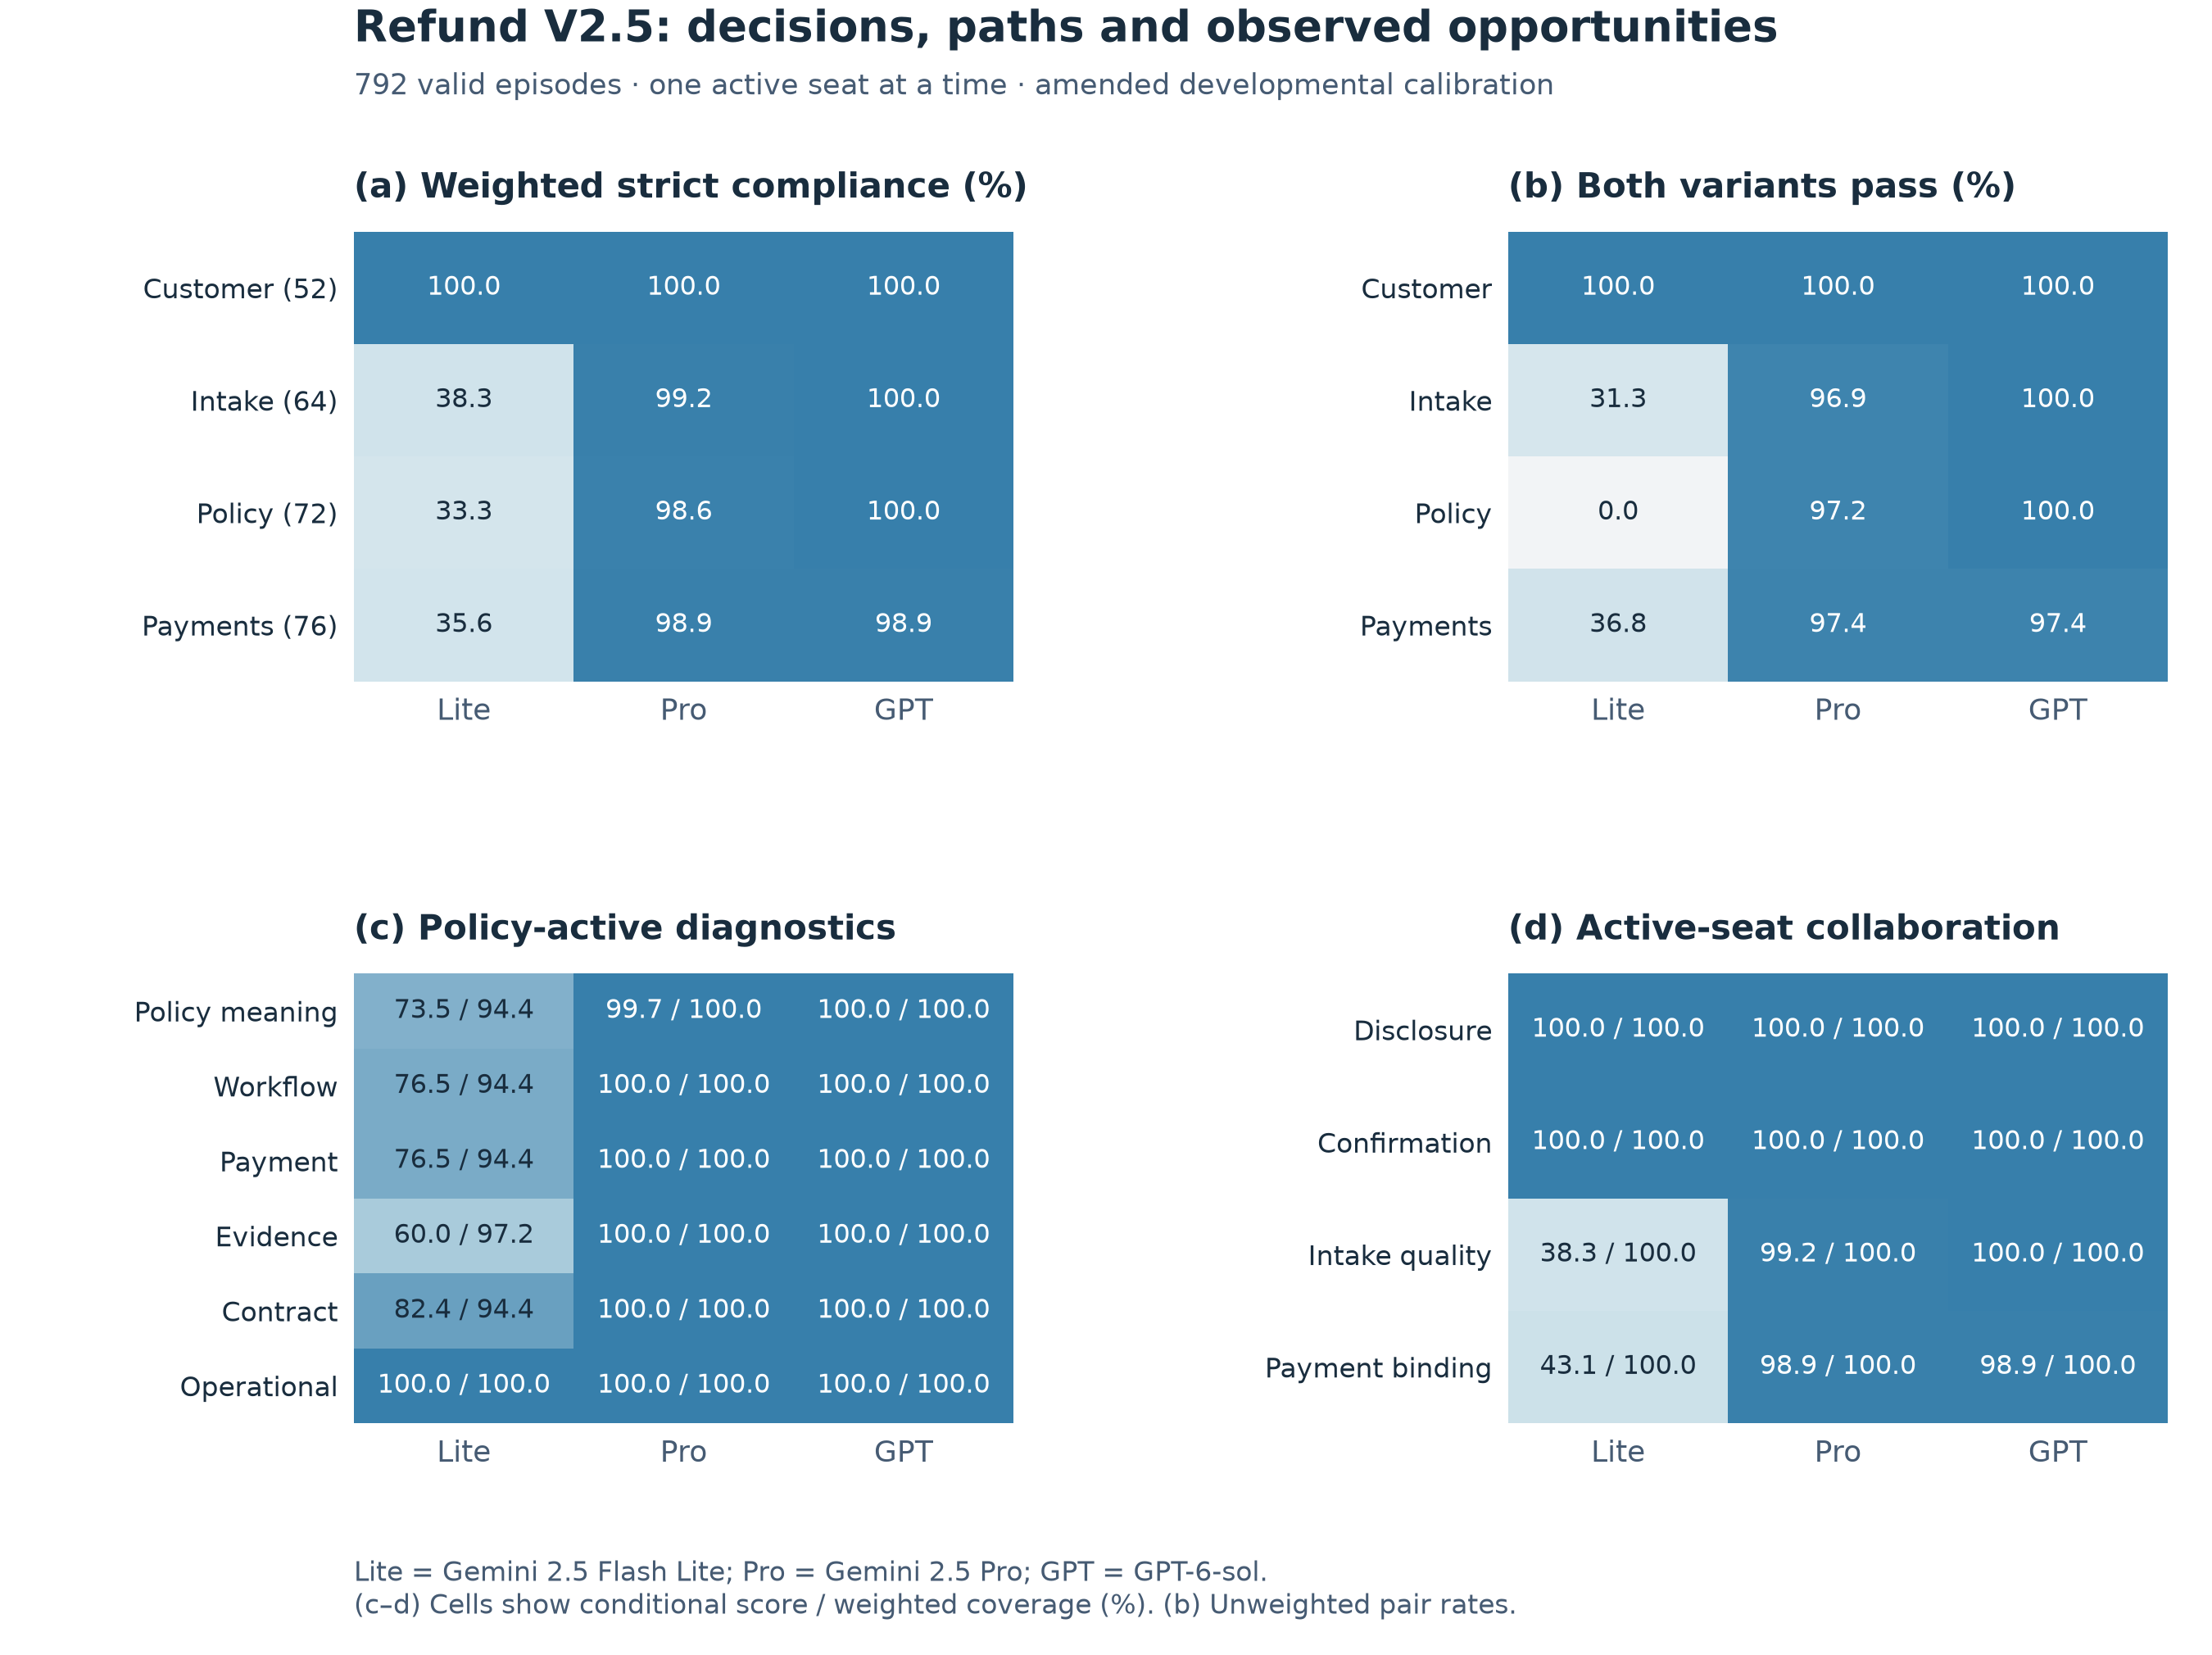
\includegraphics[width=\linewidth]{figures/refund_v25_compliance.png}
\caption{\textbf{Refund V2.5 calibration, by evaluated seat and model (Lite = Gemini 2.5 Flash Lite, Pro = Gemini 2.5
Pro, GPT = GPT-6-sol).} (a) Weighted strict compliance, with episodes per model in parentheses; (b) share of template
repeats in which both variants pass; (c, d) conditional score / weighted coverage, in percent. Panels are not added.}
\label{fig:E.1}
\end{figure}

\renewcommand{\thetable}{E.19}
\begin{longtable}[]{@{}
  >{\raggedright\arraybackslash}p{(\linewidth - 6\tabcolsep) * \real{0.2500}}
  >{\raggedright\arraybackslash}p{(\linewidth - 6\tabcolsep) * \real{0.2500}}
  >{\raggedright\arraybackslash}p{(\linewidth - 6\tabcolsep) * \real{0.2500}}
  >{\raggedright\arraybackslash}p{(\linewidth - 6\tabcolsep) * \real{0.2500}}@{}}
\caption{\textbf{Refund V2.5 calibration: the eight frozen paired contrasts, in percentage points of weighted strict compliance, with 95\% template-bootstrap intervals.}}\label{tab:E.19}\tabularnewline
\toprule\noalign{}
\begin{minipage}[b]{\linewidth}\raggedright
Seat
\end{minipage} & \begin{minipage}[b]{\linewidth}\raggedright
Contrast
\end{minipage} & \begin{minipage}[b]{\linewidth}\raggedright
Difference {[}95\% interval{]}
\end{minipage} & \begin{minipage}[b]{\linewidth}\raggedright
Holm p
\end{minipage} \\
\midrule\noalign{}
\endhead
\bottomrule\noalign{}
\endlastfoot
Customer & Pro minus Lite & 0.0 {[}0.0, 0.0{]} & 1.000 \\
Customer & GPT minus Pro & 0.0 {[}0.0, 0.0{]} & 1.000 \\
Intake & Pro minus Lite & 60.8 {[}44.2, 78.3{]} & 0.00586 \\
Intake & GPT minus Pro & 0.8 {[}0.0, 2.5{]} & 1.000 \\
Policy & Pro minus Lite & 65.3 {[}54.2, 76.4{]} & 0.0000610 \\
Policy & GPT minus Pro & 1.4 {[}0.0, 4.2{]} & 1.000 \\
Payments & Pro minus Lite & 63.3 {[}60.0, 67.8{]} & 0.00342 \\
Payments & GPT minus Pro & 0.0 {[}−3.3, 3.3{]} & 1.000 \\
\end{longtable}

The customer, intake, policy and payments seats have 52, 64, 72 and 76 episodes per model, and all 792 included
episodes have replay-audited receipts; the denominator is valid episodes, not every provider attempt. Unweighted
strict pass counts are 52, 32, 24 and 32 for Flash Lite, 52, 63, 71 and 75 for Pro, and 52, 64, 72 and 75 for
GPT-6-sol; these counts do not replace the frozen weights of Figure E.1. Requiring both variants of a pair to pass
within a repetition gives 100.0\%, 31.3\%, 0.0\% and 36.8\% for Flash Lite, 100.0\%, 96.9\%, 97.2\% and 97.4\% for Pro, and
100.0\%, 100.0\%, 100.0\% and 97.4\% for GPT-6-sol. The zero-width interval in the customer seat reflects a saturated
template pool, not certainty of equal performance on unseen worlds. In the intake seat, the scripted downstream checks
pass whenever they are reached, but Flash Lite reaches them in only 38.3\% of weighted trajectories, so that
conditional full score does not measure its policy ability. Because the counterparts are scripted, a full downstream
score in Figure E.1 does not show a capability of the evaluated model; the figure's operational row covers the 792
included episodes, not every provider attempt.

\textbf{Failure checks.} Pro has three strict failures: an intake request that names three relevant facts despite a batch
capacity of two, a one-cent allocation error in a refund whose total is nevertheless correct, and the liability error
in the policy seat described in Section 5.2. GPT-6-sol has one: it selects the correct fallback instrument but writes
it into the ticket's immutable logical refund-method field, so the error is not evidence that funds went to the wrong
destination. All four failures occur in the second repetition, and each first repetition of the same case passes.
Replaying the four recorded actions reproduces their outcomes, and replacing only the erroneous action by a
correction derived from the public rules yields four full-score trajectories. Twelve scripted positive controls pass
and fifteen injected errors are detected. These checks support the local attributions; they do not show that the
verifier has no other defects.

\textbf{Figure accounting.} Figure 5.2(d) uses the policy seat only. Its priority order, fixed after the runs, assigns
each failed episode once: first a decision attempted before the required facts, then an invalid request or no
scoreable final resolution, then an observed policy, workflow or payment mismatch, and last a remaining contract-only
error. Overlapping taxonomy tags are not added. For Flash Lite this assigns 26, 4, 18 and 0 of 72 episodes, a total
shortfall of 66.7 points; Pro has one mismatch in 72 (1.4 points), and GPT-6-sol has none. The resolution-mismatch
segment includes policy, workflow and prescribed-payment meaning, not only the four-field policy score. Some premature
candidates also have wrong fields but are counted once, under the first class. The accounting describes the first
applicable failure, not its causal effect.

\textbf{Release scope.} The figure data record the digests of the frozen configuration, the merged 792 episodes, the
analysis and the offline audit, and this paper does not change the analysis. The model outcomes remain bound to their
original versioned runner and adapter. The public release adds customer and intake panels, giving 13 public cohorts,
268 placements and 244 distinct case identifiers per seed; the 24 core cases overlap the 76-case policy panel. Its
1,072 provider-free reference trajectories (every cohort under each of the four controlled seats) complete with full
scores, independent replay and audit, and no operational exclusions. They are not 1,072 distinct worlds or additional
model observations. The earlier lower-control results on 11 cohorts (Appendix F.4) remain historical quality-control
evidence, and the expanded release has not been promoted to full publication qualification.

\subsection{Failure classes: rules and full tables}\label{failure-classes-rules-and-full-tables}

\renewcommand{\thetable}{E.4}
\begin{longtable}[]{@{}
  >{\raggedright\arraybackslash}p{(\linewidth - 2\tabcolsep) * \real{0.5000}}
  >{\raggedright\arraybackslash}p{(\linewidth - 2\tabcolsep) * \real{0.5000}}@{}}
\caption{\textbf{The shared classes.}}\label{tab:E.4}\tabularnewline
\toprule\noalign{}
\begin{minipage}[b]{\linewidth}\raggedright
Class
\end{minipage} & \begin{minipage}[b]{\linewidth}\raggedright
What happened
\end{minipage} \\
\midrule\noalign{}
\endhead
\bottomrule\noalign{}
\endlastfoot
Information not acquired & acted without information worth acquiring: signed an uninspected listing whose quality nothing it knew had settled; paid the premium or awarded the recorded supplier where the best policy tested a newcomer; decided before a required fact \\
Acted contrary to information held & the trajectory contains information (an inspection result, a landlord's reply, a sample result, revealed facts) under which the reference acts differently, and the subject did not: signed a hold that, under the landlords' pricing rule, only a lemon's landlord offers, at a rent above a lemon's value; awarded a supplier its own test showed bad; stopped after one bad newcomer where another test was worth it; tested the wrong newcomer or in the wrong order; a decision the answer key contradicts after every required fact was revealed. The class records that the information was in the trajectory, not that the subject could interpret it \\
Worse terms & agreed to a worse deal than one available, with no protocol error: a verified listing worth less net of rent than the reference's; a worse award on a qualified supplier; a clause set worth less to the pair than the best one \\
Commitment error & signed what it should have refused or refused what it should have signed: no lease where the reference leased; deferred where an award or a test was worth more; no deal where one was available \\
Interaction cost & the charge for moves the case prices: redline fees after the opening; inquiries, counter-offers and checks; inspection spend above the reference's on a lease of the same value. Any gain such a move brings appears in another class (a better clause set is smaller worse-terms loss), so this class prices the moves and does not judge them \\
Procedure and format & an action the environment rejected or could not parse; a fact request the case rejects; a format the verifier rejects \\
Operational & an episode with no measurement; counted, never scored \\
\end{longtable}

For a unit u (an episode, an action or a part of a grade, depending on the case), the shortfall is the reference's
value minus the agent's, and the rules assign it to the classes in priority order:

\[ \text{S(u) = V\textsubscript{ref}(u) − V(u) = Σ over classes c of S\textsubscript{c}(u),} \tag{E.2} \]

where c ranges over the six scored classes and each part of the loss goes to the first class whose rule it meets. The
priority order makes the decomposition an accounting identity, not a causal attribution.

\textbf{Rules per case.} \emph{Housing.} The unit is the episode (one world under one landlord kind). The shortfall is the
reachable reference's net minus the tenant's net under v15's primary measure (the reply-conditioned measure), and the
rules apply in the order procedure, contrary to information held, information not acquired, commitment error, worse
terms and interaction cost. A known lemon signed at a rent that its lemon value covers is judged on terms, because the
reference does the same. Signing a revealed lemon counts as acting contrary to information held: v15's task prompt
states how landlords price, so the acceptance that reveals a lemon follows from a stated rule. The rules are v14's.
They read seat 0's decisions from v15's seat-0 receipts, the reference is \texttt{inspect\_\allowbreak{}lowball} scored as v15's scorer
scores it, and every episode's gap reproduces the published v15 analysis. v14's class totals (Gemini \$78.9, GLM \$142.3
and Luna \$144.3 a world) remain in the source package. \emph{Procurement.} The unit is the action. Each action's loss
against the best policy (these losses sum to the decision loss) goes to a class according to what the action did. A
request to the recorded supplier counts as information not acquired only when the episode never tests a newcomer, and
as acting contrary to information held otherwise. \emph{Data center.} The unit is each part of a negotiation's grade. No
deal is a commitment error, labelled by the side that walked away. Allocation loss in a world with positive available
surplus counts as worse terms, while allocation loss in a world without positive available surplus is a harmful
agreement, which is a commitment error. Redline fees are interaction cost. Figure 5.2c separates harmful agreements
from missed beneficial deals. We count signing below one's own walk-away value separately: that individual loss is
not an additive component of joint loss, although the same agreement may also destroy joint value. \emph{Refund V2.1 (historical).} The
parts of the published gap decomposition map onto the classes: deciding before a required fact maps to information
not acquired, a wrong decision to acting contrary to information held, and re-asked or unknown facts and the null
refund method to procedure and format. The V2.5 panel instead counts each failed episode once, under the first
applicable class (Appendix E.4).

\textbf{Interpreting negotiation costs.} A redline that improves the final agreement's joint value by
\$100k while costing \$25k reduces total shortfall by \$75k: allocation loss falls by \$100k and
interaction cost rises by \$25k. The score therefore credits improvements net of their cost. The
full-information reference knows both private types and can propose the best agreement in the
free opening move. Its advantage includes negotiation costs that agents with limited information
may need to incur; the decomposition does not identify which costs were avoidable. It also does
not establish robustness to the chosen \$25k fee per additional redline. Appendix E.9 tests
scoring sensitivity by replaying the same actions at alternative fees; measuring behavioural
adaptation would require new model runs under pre-registered fee settings.

\renewcommand{\thetable}{E.5}
\begin{longtable}[]{@{}
  >{\raggedright\arraybackslash}p{(\linewidth - 18\tabcolsep) * \real{0.0769}}
  >{\raggedleft\arraybackslash}p{(\linewidth - 18\tabcolsep) * \real{0.1026}}
  >{\raggedleft\arraybackslash}p{(\linewidth - 18\tabcolsep) * \real{0.1026}}
  >{\raggedleft\arraybackslash}p{(\linewidth - 18\tabcolsep) * \real{0.1026}}
  >{\raggedleft\arraybackslash}p{(\linewidth - 18\tabcolsep) * \real{0.1026}}
  >{\raggedleft\arraybackslash}p{(\linewidth - 18\tabcolsep) * \real{0.1026}}
  >{\raggedleft\arraybackslash}p{(\linewidth - 18\tabcolsep) * \real{0.1026}}
  >{\raggedleft\arraybackslash}p{(\linewidth - 18\tabcolsep) * \real{0.1026}}
  >{\raggedleft\arraybackslash}p{(\linewidth - 18\tabcolsep) * \real{0.1026}}
  >{\raggedleft\arraybackslash}p{(\linewidth - 18\tabcolsep) * \real{0.1026}}@{}}
\caption{\textbf{Housing and Procurement, every subject (\$ per world; Housing v15 on the 260 main worlds of Table 5.2, GLM, Sol and Opus from their pre-registered addenda; Procurement on the 20 pre-registered worlds of Table 5.3, each world the mean of its two plays).}}\label{tab:E.5}\tabularnewline
\toprule\noalign{}
\begin{minipage}[b]{\linewidth}\raggedright
Class
\end{minipage} & \begin{minipage}[b]{\linewidth}\raggedleft
Housing Gemini
\end{minipage} & \begin{minipage}[b]{\linewidth}\raggedleft
Housing Luna
\end{minipage} & \begin{minipage}[b]{\linewidth}\raggedleft
Housing Sol (addendum B)
\end{minipage} & \begin{minipage}[b]{\linewidth}\raggedleft
Housing Opus (addendum B)
\end{minipage} & \begin{minipage}[b]{\linewidth}\raggedleft
Housing GLM (addendum A)
\end{minipage} & \begin{minipage}[b]{\linewidth}\raggedleft
Proc. Sol
\end{minipage} & \begin{minipage}[b]{\linewidth}\raggedleft
Proc. Opus
\end{minipage} & \begin{minipage}[b]{\linewidth}\raggedleft
Proc. Gemini
\end{minipage} & \begin{minipage}[b]{\linewidth}\raggedleft
Proc. Luna
\end{minipage} \\
\midrule\noalign{}
\endhead
\bottomrule\noalign{}
\endlastfoot
Information not acquired & −0.2 & 14.9 & 0 & 1.4 & 18.9 & 17.5 & 51.0 & 49.4 & 55.4 \\
Acted contrary to information held & 1.9 & 22.2 & 0 & 0 & 49.6 & 13.9 & 0 & 0 & 0 \\
Worse terms & 40.7 & 54.3 & 15.7 & 38.8 & 40.1 & 0 & 0 & 0 & 0.5 \\
Commitment error & 8.9 & 8.6 & −0.0 & 6.3 & 7.2 & 0 & 0 & 0 & 0 \\
Interaction cost & −0.3 & −0.1 & −0.4 & −0.4 & −0.2 & 1.1 & 0.2 & 1.9 & 2.2 \\
Procedure and format & 0 & 0 & 0 & 0 & 11.7 & 0 & 0 & 0 & 0 \\
Total & 51.1 & 99.9 & 15.3 & 46.1 & 127.3 & 32.5 & 51.2 & 51.2 & 58.1 \\
\end{longtable}

Housing's totals reproduce the published v15 differences from \texttt{inspect\_\allowbreak{}lowball} (51.13 and 99.92 \$ a world; GLM's addendum row R3, 127.32; Sol's and Opus's addendum row R, 15.34 and 46.07), and every one of the 520 main episodes per model completed, so no world is excluded. Main-world means average both landlord arms within a world. We retain negative amounts where the model beats the reference. The inspection-cost row is a residual after the earlier classes, so inspection costs already inside other classes are not counted again.

\renewcommand{\thetable}{E.6}
\begin{longtable}[]{@{}
  >{\raggedright\arraybackslash}p{(\linewidth - 16\tabcolsep) * \real{0.0857}}
  >{\raggedleft\arraybackslash}p{(\linewidth - 16\tabcolsep) * \real{0.1143}}
  >{\raggedleft\arraybackslash}p{(\linewidth - 16\tabcolsep) * \real{0.1143}}
  >{\raggedleft\arraybackslash}p{(\linewidth - 16\tabcolsep) * \real{0.1143}}
  >{\raggedleft\arraybackslash}p{(\linewidth - 16\tabcolsep) * \real{0.1143}}
  >{\raggedleft\arraybackslash}p{(\linewidth - 16\tabcolsep) * \real{0.1143}}
  >{\raggedleft\arraybackslash}p{(\linewidth - 16\tabcolsep) * \real{0.1143}}
  >{\raggedleft\arraybackslash}p{(\linewidth - 16\tabcolsep) * \real{0.1143}}
  >{\raggedleft\arraybackslash}p{(\linewidth - 16\tabcolsep) * \real{0.1143}}@{}}
\caption{\textbf{Data center development (\$k joint value lost per deal world) and historical Refund V2.1 (points of episodes unresolved).}}\label{tab:E.6}\tabularnewline
\toprule\noalign{}
\begin{minipage}[b]{\linewidth}\raggedright
Class
\end{minipage} & \begin{minipage}[b]{\linewidth}\raggedleft
DC Sol int. × Opus
\end{minipage} & \begin{minipage}[b]{\linewidth}\raggedleft
DC Opus int. × Sol
\end{minipage} & \begin{minipage}[b]{\linewidth}\raggedleft
DC Sol × firm
\end{minipage} & \begin{minipage}[b]{\linewidth}\raggedleft
DC Opus × firm
\end{minipage} & \begin{minipage}[b]{\linewidth}\raggedleft
Refund DeepSeek
\end{minipage} & \begin{minipage}[b]{\linewidth}\raggedleft
Refund Gemini 2.5 FL
\end{minipage} & \begin{minipage}[b]{\linewidth}\raggedleft
Refund GPT-5.6 Luna
\end{minipage} & \begin{minipage}[b]{\linewidth}\raggedleft
Refund Grok
\end{minipage} \\
\midrule\noalign{}
\endhead
\bottomrule\noalign{}
\endlastfoot
Information not acquired & --- & --- & --- & --- & 44.2 & 0 & 15.0 & 29.2 \\
Acted contrary to information held & --- & --- & --- & --- & 0 & 0 & 0 & 0.8 \\
Worse terms & 35.4 & 12.2 & 9.1 & 4.8 & 0 & 0 & 0 & 0 \\
Commitment error & 0 & 0 & 32.0 & 6.9 & --- & --- & --- & --- \\
Interaction cost & 46.2 & 66.3 & 80.2 & 29.8 & --- & --- & --- & --- \\
Procedure and format & 0 & 0 & 0 & 0 & 5.8 & 98.3 & 5.8 & 17.5 \\
Total & 81.5 & 78.6 & 121.3 & 41.5 & 50.0 & 98.3 & 20.8 & 47.5 \\
\end{longtable}

In these development runs, 7 of Sol's 8 lost deals against the firm script occurred when the script walked away from
Sol's last offer. Signing below one's own walk-away point, which the table does not include, occurred for Opus as
client in 12 of 52 worlds against Sol (in 4 of them Opus proposed the losing terms itself) and in 2 against the firm
script, and for Sol as client in 1 against the firm script; neither model did so as integrator.

\subsection{Two frontier agents across three cases}\label{two-frontier-agents-across-three-cases}

\renewcommand{\thetable}{E.7}
\begin{longtable}[]{@{}
  >{\raggedright\arraybackslash}p{(\linewidth - 10\tabcolsep) * \real{0.1429}}
  >{\raggedright\arraybackslash}p{(\linewidth - 10\tabcolsep) * \real{0.1429}}
  >{\raggedleft\arraybackslash}p{(\linewidth - 10\tabcolsep) * \real{0.1905}}
  >{\raggedleft\arraybackslash}p{(\linewidth - 10\tabcolsep) * \real{0.1905}}
  >{\raggedleft\arraybackslash}p{(\linewidth - 10\tabcolsep) * \real{0.1905}}
  >{\raggedright\arraybackslash}p{(\linewidth - 10\tabcolsep) * \real{0.1429}}@{}}
\caption{\textbf{Development comparisons of Opus 5.5 and Sol 6.1 on the three cases both played; Data-center confirmatory results are in Table 5.4 (v2) and Table E.16 (v1).}}\label{tab:E.7}\tabularnewline
\toprule\noalign{}
\begin{minipage}[b]{\linewidth}\raggedright
Case (worlds)
\end{minipage} & \begin{minipage}[b]{\linewidth}\raggedright
Measure
\end{minipage} & \begin{minipage}[b]{\linewidth}\raggedleft
Opus 5.5
\end{minipage} & \begin{minipage}[b]{\linewidth}\raggedleft
Sol 6.1
\end{minipage} & \begin{minipage}[b]{\linewidth}\raggedleft
Sol relative to Opus
\end{minipage} & \begin{minipage}[b]{\linewidth}\raggedright
Reference
\end{minipage} \\
\midrule\noalign{}
\endhead
\bottomrule\noalign{}
\endlastfoot
Housing (20) & tenant net per world & 291 {[}198, 383{]} & 313 {[}225, 402{]} & +23 {[}−19, +64{]} & scripted reference 331 \\
Housing, favourite a lemon (10) & tenant net per world & 155 & 200 & not tested & scripted reference 235 \\
Procurement pay-or-test (24) & given up per world & 5.4 {[}1.2, 10.6{]} & 1.0 {[}0.2, 2.1{]} & 4.4 {[}0.6, 9.0{]} less given up & best policy gives up 0 \\
Procurement, record evaluation set (18) & worlds solved & 18 & 16 & regret −20 {[}−48, +7{]} (Opus lower) & informed policy 18 \\
Data center development, firm population (52) & earns, integrator / client (\$k) & 122 / 107 & 139 / 130 & +17 {[}−10, +44{]} / +23 {[}−2, +48{]} & first-offer stand-in 122 / 114 \\
Data center development, head to head (52) & earns, integrator / client (\$k) & 60 / 25 & 308 / 276 & +248 / +251 & \\
\end{longtable}

\subsection{Current shortfall panels: scope and uncertainty}\label{current-shortfall-panels-scope-and-uncertainty}

Figure 5.2 is descriptive accounting computed after the runs, not an additional pre-registered test. Its Data-center
panel uses all 80 included worlds of v2, including 8 with no positive available surplus, whereas Table 5.4's earnings
contrasts use the 72 worlds with a deal. Both focal roles receive equal weight within each world, after the
integrator's two plays against the firm client are averaged. We do not add individual signings below the walk-away
point to joint loss: as integrator against the firm client, Opus signed below its outside option in 2 of 160 plays and
Sol in none, and as client neither model did so in 80. Table E.6 preserves the earlier development decomposition on
its 52 deal worlds, and Table E.17 gives v1's decomposition by pairing.

\renewcommand{\thetable}{E.8}
\begin{longtable}[]{@{}
  >{\raggedright\arraybackslash}p{(\linewidth - 10\tabcolsep) * \real{0.1304}}
  >{\raggedleft\arraybackslash}p{(\linewidth - 10\tabcolsep) * \real{0.1739}}
  >{\raggedleft\arraybackslash}p{(\linewidth - 10\tabcolsep) * \real{0.1739}}
  >{\raggedleft\arraybackslash}p{(\linewidth - 10\tabcolsep) * \real{0.1739}}
  >{\raggedleft\arraybackslash}p{(\linewidth - 10\tabcolsep) * \real{0.1739}}
  >{\raggedleft\arraybackslash}p{(\linewidth - 10\tabcolsep) * \real{0.1739}}@{}}
\caption{\textbf{Data-center joint loss by pairing in v2 (\$ thousands per world, all 80 worlds; the integrator's two plays against the firm client averaged within each world).}}\label{tab:E.8}\tabularnewline
\toprule\noalign{}
\begin{minipage}[b]{\linewidth}\raggedright
Integrator / client
\end{minipage} & \begin{minipage}[b]{\linewidth}\raggedleft
Inferior clauses
\end{minipage} & \begin{minipage}[b]{\linewidth}\raggedleft
Harmful agreement
\end{minipage} & \begin{minipage}[b]{\linewidth}\raggedleft
Missed deal
\end{minipage} & \begin{minipage}[b]{\linewidth}\raggedleft
Redline fees
\end{minipage} & \begin{minipage}[b]{\linewidth}\raggedleft
Total
\end{minipage} \\
\midrule\noalign{}
\endhead
\bottomrule\noalign{}
\endlastfoot
Opus / Sol & 12.6 & 0.0 & 24.3 & 74.4 & 111.4 \\
Sol / Opus & 22.4 & 0.0 & 26.1 & 68.1 & 116.7 \\
Opus / firm & 2.2 & 0.0 & 9.1 & 40.0 & 51.3 \\
Sol / firm & 1.7 & 0.0 & 45.9 & 73.9 & 121.6 \\
Firm / Opus & 17.0 & 0.0 & 48.3 & 50.6 & 115.9 \\
Firm / Sol & 12.4 & 0.0 & 53.6 & 92.8 & 158.8 \\
\end{longtable}

\renewcommand{\thetable}{E.9}
\begin{longtable}[]{@{}
  >{\raggedright\arraybackslash}p{(\linewidth - 8\tabcolsep) * \real{0.1875}}
  >{\raggedleft\arraybackslash}p{(\linewidth - 8\tabcolsep) * \real{0.2500}}
  >{\raggedright\arraybackslash}p{(\linewidth - 8\tabcolsep) * \real{0.1875}}
  >{\raggedright\arraybackslash}p{(\linewidth - 8\tabcolsep) * \real{0.1875}}
  >{\raggedright\arraybackslash}p{(\linewidth - 8\tabcolsep) * \real{0.1875}}@{}}
\caption{\textbf{Distribution of total shortfall (each case's own units). The Refund rows are the historical V2.1 panel; the V2.5 results are in Table E.19.}}\label{tab:E.9}\tabularnewline
\toprule\noalign{}
\begin{minipage}[b]{\linewidth}\raggedright
Case / subject
\end{minipage} & \begin{minipage}[b]{\linewidth}\raggedleft
Units (n)
\end{minipage} & \begin{minipage}[b]{\linewidth}\raggedright
Mean {[}95\% interval{]}
\end{minipage} & \begin{minipage}[b]{\linewidth}\raggedright
Median {[}Q1, Q3{]}
\end{minipage} & \begin{minipage}[b]{\linewidth}\raggedright
Zero / negative units
\end{minipage} \\
\midrule\noalign{}
\endhead
\bottomrule\noalign{}
\endlastfoot
Housing: Gemini 3.8 Flash & 260 & 51.1 {[}38.3, 63.9{]} & 29.9 {[}0.0, 98.3{]} & 60 / 45 \\
Housing: GPT-6 Luna & 260 & 99.9 {[}83.8, 116.0{]} & 72.1 {[}0.0, 167.6{]} & 46 / 32 \\
Housing: Sol 6.1 (addendum B) & 260 & 15.3 {[}6.2, 24.5{]} & 0.0 {[}0.0, 53.7{]} & 78 / 59 \\
Housing: Opus 5.5 (addendum B) & 260 & 46.1 {[}33.9, 58.2{]} & 27.8 {[}0.0, 96.0{]} & 61 / 47 \\
Housing: GLM 5.3 Flash (addendum A) & 260 & 127.3 {[}105.2, 149.4{]} & 79.9 {[}0.0, 212.8{]} & 36 / 39 \\
Procurement: Sol 6.1 & 20 & 32.5 {[}23.8, 41.3{]} & 33.3 {[}21.5, 48.7{]} & 0 / 0 \\
Procurement: Opus 5.5 & 20 & 51.2 {[}46.3, 56.2{]} & 50.2 {[}45.1, 57.7{]} & 0 / 0 \\
Procurement: Gemini 3.8 Flash & 20 & 51.2 {[}46.3, 56.2{]} & 50.2 {[}45.1, 57.7{]} & 0 / 0 \\
Procurement: GPT-6 Luna & 20 & 58.1 {[}52.3, 63.9{]} & 57.2 {[}50.4, 67.1{]} & 0 / 0 \\
Data center: Opus 5.5 & 80 & 83.6 {[}68.8, 98.4{]} & 57.2 {[}27.8, 137.3{]} & 0 / 0 \\
Data center: Sol 6.1 & 80 & 140.2 {[}120.6, 159.7{]} & 117.3 {[}87.5, 189.8{]} & 4 / 0 \\
Refund V2.1: GPT-5.6 Luna & 6 & 20.8 {[}-1.0, 42.7{]} & 20.0 {[}3.8, 28.8{]} & 2 / 0 \\
Refund V2.1: Gemini 2.5 Flash Lite & 6 & 98.3 {[}94.0, 102.6{]} & 100.0 {[}100.0, 100.0{]} & 0 / 0 \\
\end{longtable}

Opus and Gemini bought from the recorded supplier in every play, so their Procurement rows coincide. The intervals
are Student t intervals over independent worlds (for Housing after averaging the arms, and for Data center after
averaging the focal roles), or over the six fixed Refund V2.1 cases after averaging 20 episodes per case. They describe
variation in these panels; they do not establish a model ranking or coverage of a field population. They are
descriptive intervals that we derived afterwards, not replacements for the campaigns' pre-registered analyses. A
Refund interval can exceed the score's 0--100 bounds; we leave it untruncated to expose the weakness of an
approximation with six fixed cases. Housing has one retained run per world and landlord arm, so its run-to-run variance is unmeasured. Procurement and
Data center have two plays per world: the two plays of a world scored identically in 7 to 20 of the 20 Procurement
worlds, depending on the model, and ended identically in 47 (Opus) and 28 (Codex) of the 80 Data center worlds
(Appendix F.1). Refund V2.1 has repeated episodes within fixed cases, and the derived
evidence retains its per-case outcome distributions. The source package includes component-level intervals,
distributions, per-world amounts and input digests, together with a reproduction script that makes no provider
call.

\subsection{Exact values for Figure 5.2}\label{exact-values-for-figure-5.2}

The figure draws the estimates below. Each component keeps its case's native units and classification rules, and
the figure adds no new analysis or cross-case aggregate.

\textbf{Table E.10. Shortfall by case. Housing uses v15 (Table 5.2) under its primary measure; Data center uses v2, the comparison of Table 5.4; Procurement uses the 20 pre-registered worlds of Table 5.3. Refund uses the policy seat of the V2.5 calibration.}

\textbf{(a) Housing}

Dollars per main world below the reachable scripted reference (\texttt{inspect\_\allowbreak{}lowball}), under v15's measure v2.

\begin{longtable}[]{@{}
  >{\raggedright\arraybackslash}p{(\linewidth - 10\tabcolsep) * \real{0.1304}}
  >{\raggedleft\arraybackslash}p{(\linewidth - 10\tabcolsep) * \real{0.1739}}
  >{\raggedleft\arraybackslash}p{(\linewidth - 10\tabcolsep) * \real{0.1739}}
  >{\raggedleft\arraybackslash}p{(\linewidth - 10\tabcolsep) * \real{0.1739}}
  >{\raggedleft\arraybackslash}p{(\linewidth - 10\tabcolsep) * \real{0.1739}}
  >{\raggedleft\arraybackslash}p{(\linewidth - 10\tabcolsep) * \real{0.1739}}@{}}
\toprule\noalign{}
\begin{minipage}[b]{\linewidth}\raggedright
Component
\end{minipage} & \begin{minipage}[b]{\linewidth}\raggedleft
Gemini 3.8 Flash
\end{minipage} & \begin{minipage}[b]{\linewidth}\raggedleft
GPT-6 Luna
\end{minipage} & \begin{minipage}[b]{\linewidth}\raggedleft
Sol 6.1 (Codex, addendum B)
\end{minipage} & \begin{minipage}[b]{\linewidth}\raggedleft
Opus 5.5 (Claude Code, addendum B)
\end{minipage} & \begin{minipage}[b]{\linewidth}\raggedleft
GLM 5.3 Flash (addendum A)
\end{minipage} \\
\midrule\noalign{}
\endhead
\bottomrule\noalign{}
\endlastfoot
Information not acquired & −0.2 & 14.9 & 0.0 & 1.4 & 18.9 \\
Contrary to held information & 1.9 & 22.2 & 0.0 & 0.0 & 49.6 \\
Worse lease terms & 40.7 & 54.3 & 15.7 & 38.8 & 40.1 \\
Lease commitment error & 8.9 & 8.6 & −0.0 & 6.3 & 7.2 \\
Procedure or format & 0.0 & 0.0 & 0.0 & 0.0 & 11.7 \\
Inspection cost & −0.3 & −0.1 & −0.4 & −0.4 & −0.2 \\
\textbf{Total shortfall} & \textbf{51.1} & \textbf{99.9} & \textbf{15.3} & \textbf{46.1} & \textbf{127.3} \\
\end{longtable}

The two landlord arms are averaged within each of the 260 main worlds, and no episode is missing. GLM (addendum A) and the two command-line agents (addendum B) played in pre-registered addenda outside v15's contrasts. GLM's procedure losses are actions the environment refused, chiefly malformed commits (\$5.7 a world, 14 episodes) and offers on listings already taken (\$2.1, 5 episodes). Negative amounts mean that the model did better than the reference in that class; they are not drawn in Figure 5.2.

\textbf{(b) Procurement}

Dollars per world below the best policy given the available information, on the 20 pre-registered worlds of Table 5.3 with two plays each.

\begin{longtable}[]{@{}
  >{\raggedright\arraybackslash}p{(\linewidth - 8\tabcolsep) * \real{0.1579}}
  >{\raggedleft\arraybackslash}p{(\linewidth - 8\tabcolsep) * \real{0.2105}}
  >{\raggedleft\arraybackslash}p{(\linewidth - 8\tabcolsep) * \real{0.2105}}
  >{\raggedleft\arraybackslash}p{(\linewidth - 8\tabcolsep) * \real{0.2105}}
  >{\raggedleft\arraybackslash}p{(\linewidth - 8\tabcolsep) * \real{0.2105}}@{}}
\toprule\noalign{}
\begin{minipage}[b]{\linewidth}\raggedright
Component
\end{minipage} & \begin{minipage}[b]{\linewidth}\raggedleft
Sol 6.1
\end{minipage} & \begin{minipage}[b]{\linewidth}\raggedleft
Opus 5.5
\end{minipage} & \begin{minipage}[b]{\linewidth}\raggedleft
Gemini 3.8 Flash
\end{minipage} & \begin{minipage}[b]{\linewidth}\raggedleft
GPT-6 Luna
\end{minipage} \\
\midrule\noalign{}
\endhead
\bottomrule\noalign{}
\endlastfoot
Information not acquired & 17.5 & 51.0 & 49.4 & 55.4 \\
Contrary to held information & 13.9 & 0.0 & 0.0 & 0.0 \\
Worse terms & 0.0 & 0.0 & 0.0 & 0.5 \\
Award checks & 1.1 & 0.2 & 1.9 & 2.2 \\
\textbf{Total shortfall} & \textbf{32.5} & \textbf{51.2} & \textbf{51.2} & \textbf{58.1} \\
\end{longtable}

The panel shows all four models, with each world the mean of its two plays. Sol runs through Codex, Opus through Claude Code, and Gemini and Luna through OpenRouter. We re-derived the decision loss from every play's replayed trace and matched every world against the read-outs. The pre-registered rules file an award's whole loss under information not acquired when the award came before a worthwhile newcomer test, including the part caused by a worse quantity. For Luna, which ordered 50 units where 55 was best in 15 of 40 plays, that part is \$6.33 a world; if the loss were split into its timing and terms parts, Luna's worse-terms loss would be \$6.85, its whole loss beyond paying the premium. The other three models made no such awards.

\textbf{(c) Data center}

Thousands of dollars of joint value lost relative to the full-information bound, in v2 against the firm counterparts.

\begin{longtable}[]{@{}
  >{\raggedright\arraybackslash}p{(\linewidth - 4\tabcolsep) * \real{0.2727}}
  >{\raggedleft\arraybackslash}p{(\linewidth - 4\tabcolsep) * \real{0.3636}}
  >{\raggedleft\arraybackslash}p{(\linewidth - 4\tabcolsep) * \real{0.3636}}@{}}
\toprule\noalign{}
\begin{minipage}[b]{\linewidth}\raggedright
Component
\end{minipage} & \begin{minipage}[b]{\linewidth}\raggedleft
Opus 5.5
\end{minipage} & \begin{minipage}[b]{\linewidth}\raggedleft
Sol 6.1
\end{minipage} \\
\midrule\noalign{}
\endhead
\bottomrule\noalign{}
\endlastfoot
Inferior contract clauses & 9.6 & 7.1 \\
Harmful agreement & 0.0 & 0.0 \\
Missed beneficial deal & 28.7 & 49.7 \\
Redline fees & 45.3 & 83.4 \\
\textbf{Total shortfall} & \textbf{83.6} & \textbf{140.2} \\
\end{longtable}

All 80 worlds, with both focal roles averaged within each world. Joint outcomes reflect both parties' actions.

\textbf{(d) Refund}

Percentage points below strict trajectory compliance in the policy seat of the V2.5 calibration.

\begin{longtable}[]{@{}
  >{\raggedright\arraybackslash}p{(\linewidth - 6\tabcolsep) * \real{0.2000}}
  >{\raggedleft\arraybackslash}p{(\linewidth - 6\tabcolsep) * \real{0.2667}}
  >{\raggedleft\arraybackslash}p{(\linewidth - 6\tabcolsep) * \real{0.2667}}
  >{\raggedleft\arraybackslash}p{(\linewidth - 6\tabcolsep) * \real{0.2667}}@{}}
\toprule\noalign{}
\begin{minipage}[b]{\linewidth}\raggedright
Component
\end{minipage} & \begin{minipage}[b]{\linewidth}\raggedleft
Gemini 2.5 Flash Lite
\end{minipage} & \begin{minipage}[b]{\linewidth}\raggedleft
Gemini 2.5 Pro
\end{minipage} & \begin{minipage}[b]{\linewidth}\raggedleft
GPT-6-sol
\end{minipage} \\
\midrule\noalign{}
\endhead
\bottomrule\noalign{}
\endlastfoot
Required facts skipped & 36.1 & 0.0 & 0.0 \\
Procedure or format & 5.6 & 0.0 & 0.0 \\
Resolution mismatch & 25.0 & 1.4 & 0.0 \\
\textbf{Total shortfall} & \textbf{66.7} & \textbf{1.4} & \textbf{0.0} \\
\end{longtable}

72 episodes per model; each failed episode is counted once, under the first applicable class (Appendix E.4). The
historical V2.1 panel (GPT-5.6 Luna 20.8, Gemini 2.5 Flash Lite 98.3 points) is in Tables E.6 and E.9. In it, Flash
Lite asked again for a fact it had already been given in 81\% of its episodes, which ended the case with no decision
(80.8 of its 98.3 points), and in most of the rest wrote the refund method as null where the format requires ``none''
(16.7 points); it reached the answer key's outcome in 18\% of episodes and a wrong outcome in none.

We omit rows that are zero for every displayed model, and rounded components may not add up to rounded totals.
Signing below one's walk-away value is a separate, individual outcome. In v2 neither model signed below its walk-away
value as client, whether against the firm integrator or head to head (0 of 80 each); as integrator against the firm
client, Opus signed below its outside option in 2 of 160 plays and Sol in none. Table E.16 gives v1's counts.

\subsection{Negotiation fees in v1: fixed-action sensitivity}\label{negotiation-fees-in-v1-fixed-action-sensitivity}

We replayed all 240 valid firm-population negotiations of v1 (Table E.16; 60 worlds, two models and two focal seats)
at six fees per paid redline: \$0, \$5k, \$12.5k, \$25k, \$50k and \$100k. All original final states and six score leaves
matched the saved states and receipts. The 1,440 fee-specific trajectories used the environment's own transition and
scoring functions and held offers, clauses, notes, signatures and walk-aways fixed. This is an exploratory analysis
performed after the runs, not another pre-registered test or a model rerun. The opening move remains free of fees. v2
pre-registered a smaller replay of the same kind (Section 5.2).

The two samples answer different questions. v1's joint loss covers all 60 worlds, whereas its pre-registered earnings
contrast (Table E.16) uses the 45 worlds with positive available joint surplus. ``Deal-feasible'' describes those worlds,
including negotiations in them that ended without agreement; it does not select only signed contracts. Means first
average both focal seats within a world and then average across worlds, so the independent unit is the world, not each
correlated seat observation.

\renewcommand{\thetable}{E.11}
\begin{longtable}[]{@{}
  >{\raggedright\arraybackslash}p{(\linewidth - 6\tabcolsep) * \real{0.2000}}
  >{\raggedleft\arraybackslash}p{(\linewidth - 6\tabcolsep) * \real{0.2667}}
  >{\raggedleft\arraybackslash}p{(\linewidth - 6\tabcolsep) * \real{0.2667}}
  >{\raggedleft\arraybackslash}p{(\linewidth - 6\tabcolsep) * \real{0.2667}}@{}}
\caption{\textbf{Fee sensitivity on the 45 deal-feasible worlds (\$ thousands per world; fixed actions). Sol earnings lead is Sol minus Opus against the firm population. Lower joint loss is better; a positive earnings lead favors Sol.}}\label{tab:E.11}\tabularnewline
\toprule\noalign{}
\begin{minipage}[b]{\linewidth}\raggedright
Fee per redline
\end{minipage} & \begin{minipage}[b]{\linewidth}\raggedleft
Sol joint loss
\end{minipage} & \begin{minipage}[b]{\linewidth}\raggedleft
Opus joint loss
\end{minipage} & \begin{minipage}[b]{\linewidth}\raggedleft
Sol earnings lead
\end{minipage} \\
\midrule\noalign{}
\endhead
\bottomrule\noalign{}
\endlastfoot
0 & 38.9 & 28.5 & +54.8 \\
5 & 56.0 & 35.6 & +49.1 \\
12.5 & 81.7 & 46.2 & +40.6 \\
25 & 124.4 & 63.8 & +26.4 \\
50 & 210.0 & 99.1 & -1.9 \\
100 & 381.1 & 169.6 & -58.6 \\
\end{longtable}

On these 45 worlds, fees amplify Sol's disadvantage in joint loss but do not create it: Opus retains the lower loss at
zero fees. Sol's own earnings lead, by contrast, grows when fees are removed. Because behaviour is held fixed, each
model's earnings are a linear function of the fee, and the two models' earnings are equal at approximately \$48.3k per
redline. This threshold describes the recorded actions; it is neither an optimal fee nor a prediction of how either
agent would respond to a different fee.

\renewcommand{\thetable}{E.12}
\begin{longtable}[]{@{}
  >{\raggedright\arraybackslash}p{(\linewidth - 4\tabcolsep) * \real{0.2727}}
  >{\raggedleft\arraybackslash}p{(\linewidth - 4\tabcolsep) * \real{0.3636}}
  >{\raggedleft\arraybackslash}p{(\linewidth - 4\tabcolsep) * \real{0.3636}}@{}}
\caption{\textbf{Joint-loss sensitivity across all 60 worlds (\$ thousands per world; fixed actions). This is v1's full population, including 15 worlds without positive available joint surplus.}}\label{tab:E.12}\tabularnewline
\toprule\noalign{}
\begin{minipage}[b]{\linewidth}\raggedright
Fee per redline
\end{minipage} & \begin{minipage}[b]{\linewidth}\raggedleft
Sol joint loss
\end{minipage} & \begin{minipage}[b]{\linewidth}\raggedleft
Opus joint loss
\end{minipage} \\
\midrule\noalign{}
\endhead
\bottomrule\noalign{}
\endlastfoot
0 & 31.1 & 42.3 \\
5 & 45.6 & 48.0 \\
12.5 & 67.3 & 56.6 \\
25 & 103.4 & 70.8 \\
50 & 175.7 & 99.4 \\
100 & 320.3 & 156.5 \\
\end{longtable}

Across all 60 worlds, fees contribute 69.9\% of Sol's and 40.3\% of Opus's total joint loss at \$25k per redline. On this
population the joint-loss ranking reverses without fees, with equality near \$6.4k per redline, so the 45-world result
cannot establish a fee-independent ranking for the full evaluation set. On the 45-world subset, the corresponding fee
shares are 68.8\% and 55.3\%.

\textbf{Useful changes and limits.} Among the paid redlines that the models authored in the 45 deal-feasible worlds, 23 of
Sol's 150 and 5 of Opus's 48 increased the immediate full-information clause value by more than the \$25k fee. One Sol
redline improved clause value by \$87.5k, a net improvement of \$62.5k. These are local comparisons: an edit may later be
undone, and a negotiation may remain unsigned. This count of clause value does not capture price concessions or the
information value of negotiating. The fee shares include both parties' fees, whereas these counts include only the
focal model's edits. The full-information reference keeps its advantage, and this analysis neither validates the fee's
empirical calibration nor measures adaptation to it.

The source package retains the supplied analysis, its reproduced outputs, its input hashes and the specific redline
discussed above. The reproduction uses the retained campaign logs, which the compact package does not include in
full.

\subsection{TERMS-Bench reimplementation: a reproduction in progress}\label{terms-bench-reimplementation-a-reproduction-in-progress}

This is a negative result in progress, not evidence for the four cases. It shows that an external benchmark's
environment and counterparts can run as a family on AERead's runtime, and what a faithful port requires.

TERMS-Bench evaluates bilateral price negotiation against counterparts whose type is hidden \citep{zhang2026termsbench}. We reimplemented,
from the paper's description, its alternating-offer environment, three of its six counterpart families (Candid,
Taciturn and Expressive) and four of its measures as one AERead family. The counterpart runs as a scripted seat, and
its random draws are sealed each turn, so replay recomputes the counterpart's moves as well as the scores. We did not
implement the Oracle-Cue reference or the gap measures built on it, the urgency regime, type-belief error or the other
three families, and counterpart messages are templates. The corpus has 30 cases, 15 with a zone of agreement and 15
without, each played once.

\renewcommand{\thetable}{E.18}
\begin{longtable}[]{@{}
  >{\raggedright\arraybackslash}p{(\linewidth - 8\tabcolsep) * \real{0.1579}}
  >{\raggedleft\arraybackslash}p{(\linewidth - 8\tabcolsep) * \real{0.2105}}
  >{\raggedleft\arraybackslash}p{(\linewidth - 8\tabcolsep) * \real{0.2105}}
  >{\raggedleft\arraybackslash}p{(\linewidth - 8\tabcolsep) * \real{0.2105}}
  >{\raggedleft\arraybackslash}p{(\linewidth - 8\tabcolsep) * \real{0.2105}}@{}}
\caption{\textbf{TERMS-Bench reimplementation: two of the paper's agents on the same 30 cases against scripted
counterparts, beside the paper's values. Agreement and surplus are computed over the cases with a zone of agreement
(15 for GPT-4o-mini, 12 for GLM-5.1).}}\label{tab:E.18}\tabularnewline
\toprule\noalign{}
\begin{minipage}[b]{\linewidth}\raggedright
\end{minipage} & \begin{minipage}[b]{\linewidth}\raggedleft
GPT-4o-mini
\end{minipage} & \begin{minipage}[b]{\linewidth}\raggedleft
GLM-5.1
\end{minipage} & \begin{minipage}[b]{\linewidth}\raggedleft
Paper: GPT-4o-mini
\end{minipage} & \begin{minipage}[b]{\linewidth}\raggedleft
Paper: GLM-5.1
\end{minipage} \\
\midrule\noalign{}
\endhead
\bottomrule\noalign{}
\endlastfoot
Agreement rate where a deal exists (AGR+) & 0.80 & 1.00 & 0.522 & 0.951 \\
Surplus efficiency (SE+) & 0.035 & 0.458 & 0.196 & 0.668 \\
Conditional surplus efficiency (CSE+) & 0.044 & 0.458 & 0.363 & 0.721 \\
\end{longtable}

The paper's surplus efficiency comes from its Table 16 (overlap regime, mean of the three families played here); its
agreement and conditional surplus efficiency come from its Table 2, which pools six families and three regimes, so
those two comparisons are looser. GLM-5.1 has 12 cases because its three malformed moves removed those episodes.

The reimplementation orders the two agents as the paper does on all three measures, but absolute levels are lower for
both, and for a third model. A review of the port after these runs traced the shift to four departures from the
paper's protocol rather than to the agent, whose interface in the paper is also one stateless call per round. First,
our prompt does not state the agent's payoff or the rule against accepting above its reservation value. Second, its
observation differs from the paper's. Third, a malformed move removes the episode where the paper applies a fallback;
under that fallback, GLM-5.1's surplus efficiency would be 0.520 over all 15 cases. Fourth, our price range and zone
widths are wider than the paper's.

\textbf{The reproduction.} We have built a pre-registered reproduction with those fixes, and it stopped at its first check: one of the paper's fixed-concession baselines (FC10) scores 0.307 here against the paper's 0.266, while
the other two match. The paper states how much the baselines concede (1\%, 10\% or 30\% of the remaining distance per
offer) but not how they open or accept. No agent has played the reproduction. The paper reports critical violations
by GLM-5.1 in 5\% of cases without a zone of agreement for these three families; at that rate, 15 such cases would show
none about half the time, and ours showed none. The port also exposed a harness effect. On one provider route, any
specified reasoning budget suppressed deliberation, and GLM 5.3 Flash breached its own reservation value in 13 of
30 cases, against the paper's band of 0 to 2.06\%. With no reasoning setting specified, it breached in 2 of 30 and its
surplus efficiency rose from 0.40 to 0.53; the comparison above uses that setting. This is why the reasoning condition
is part of each run's frozen configuration. The runtime's support for the scripted seat that this family uses is now
on the main branch.

\section{Quality control in detail}\label{quality-control-in-detail}

This appendix describes only the checks that we built and applied to the four cases, with two caveats that apply
throughout. First, the initial quality-control profiles and reference-run tests were written after development; only
the agreement's confirmatory run followed its profile and a dry run that made no provider call. Second, we do not
describe rules of the quality-control standard that were not applied to these cases.

\subsection{Profiles and gates}\label{profiles-and-gates}

\begin{sloppypar}
The quality-control standard defines six quality-control gates, together with the rule that a change to any bound
input reopens them, and a repository test rejects a registered family that has no profile. Each of the four current
designs now has a section in its family's profile with a typed status and a blocker for each gate (Table F.1), and
none passes Gates 1 to 5. Housing v14 is \texttt{partial} throughout (v15, discussed below, passes four of the five).
Procurement's harder evaluation set, used in Table 5.3, passes Gates 0, 1, 2, 3 and 5 and is \texttt{partial} at Gate 4
(profile section 8.2). Its environment and its registration with the runtime reached the main branch on 20 October,
the registration by the owner's override without a review by someone other than its author. Its 12 published bundles
replay through the runtime's command line, 432 of 432 receipts, among them 100 from five scripted baselines that
played the pre-registered worlds with no model, each scoring exactly as the reference scores its moves. Gate 4 stays
\texttt{partial} because the command-line agents take no seed. Gate 1 passes on the exact-reference route that the standard
added on 21 October: the reference is exact, and the six shortcuts that the profile names (paying the premium, three
fixed testing rules, the one-step rule and the kind-blind shortcut, the last two found in earlier versions) each lose
at least \$10 in every pre-registered world. Rules that do make the decision come closer: looking two newcomers ahead
loses \$8.38 a world, and as little as \$0.09 in one world. Before the route existed, we tried to establish measured
headroom with a frozen control that tests, pre-registered before its plays. The control tested but lost to the
kind-blind shortcut, so by that route only 2 of the 20 pre-registered worlds passed (Appendix E.4). A control weaker
than the shortcuts measures itself rather than the worlds, which is why the standard now uses the exact reference
where a case has one. The models' two plays of a world scored identically in all 20 worlds for Opus and Gemini and in 7
for Sol, so the effective sample is the 20 worlds, as the world-mean intervals assume. The earlier pay-or-test v1
evaluation set (Table E.14) fails Gates 1 and 3. v2 passes the scripted Gate 3 checks and its screen meets the
exact-reference route, but its pilot stopped at sizing and the case moved to v3 (Appendix F.4). The agreement's
development sets fail Gate 1 because inclusion and type assignment were confounded. Its first confirmatory run (v1)
used the included evaluation set, which is still \texttt{partial} at Gate 1 because of the client seat's construct limit and
incomplete measured-headroom qualification (Appendix F.2). Refund V2.5 fails Gate 3 on its lower controls (Appendix
F.4) and is \texttt{partial} at Gates 1, 2 and 4: a constant full refund solves 38 of its 180 policy cases, its schema accepts
a null refund method that its verifier then fails, and no adapter admits a model profile. Its developmental
calibration with three models (Section 5.1) is exploratory rather than pre-registered, so Gate 5 has not run, and the
expanded public release is qualified only for environment conformance.
\end{sloppypar}

We pre-registered and ran Housing v15 after these profiles were first written. It passes Gates 1, 2, 3 and 5 and is
\texttt{partial} at Gate 4:

\begin{itemize}
\tightlist
\item
  \textbf{Gate 1.} Its evaluation set is screened for headroom against \texttt{inspect\_\allowbreak{}then\_\allowbreak{}sign}, and its holdout changes a
  mechanism. Scored per world afterwards, every rule that skips the decision loses at least \$25 to the best informed
  tenant in every world (the smallest losses are \$28.06 for never trading, \$92.37 for signing anything, and \$25.69 for
  inspecting and then signing at the asking rent). \texttt{inspect\_\allowbreak{}lowball}, which inspects the favourite, offers \$0 and signs
  the counter-offer when the inspected value covers it, comes within \$25 of the reference in 229 of 260 worlds and
  equals it in all 60 worlds with a sound favourite. The headroom this evaluation set leaves therefore lies in carrying
  out a simple procedure, and every model falls short of that rule on average (Table 5.2).
\item
  \textbf{Gate 2.} We sealed a bundle of golden receipts through its builder, and all 1,720 episodes replay.
\item
  \textbf{Gate 3.} Its beatability rule was pre-registered before any result, both models pass it, and its receipts score
  the tenant who decides.
\item
  \textbf{Gate 5.} Its sizing record and its A/A arm preceded the freeze of the configuration.
\item
  \textbf{Gate 4, partial.} The pre-registered one-call probe of each model profile ran only after the freeze. It found
  structured output working and both reasoning tiers in effect: every sealed call's raw response carries the
  provider's count of reasoning tokens, which the kernel's OpenRouter client does not copy into its own field.
\end{itemize}

The agreement's v2 confirmatory run (Table 5.4) passes Gate 3 for its integrator seat: the price-only rule leaves
headroom in every deal world by construction, the best informed integrator earns far more than either model, and the
evaluation set separates the models. It is \texttt{partial} at Gates 0, 1, 2, 4 and 5. Its registry entry awaits a review by
someone other than its author and its code is not yet on the main branch, so replay through the runtime's command line
has not run. Its grid reference is a lower bound, so the exact-reference route does not apply, and a frozen control played on the
already frozen evaluation set could only count the worlds that pass. Gate 1 can therefore pass only on a new
evaluation set with an exact reference and a shortcut screen in every world; the client seat also retains its
construct limit. Scoring every scripted integrator rule against the grid reference shows what a new set must remove: a shortcut comes within \$25k of it in 12 of the 80 worlds, namely all 8 in which no deal is possible (walking
away earns the reference, and every scripted rule walks away) and 4 of the 72 deal worlds, three of which have a total
ceiling below \$25k. The shortcuts still lose \$104.8k to \$205.2k per deal world on average, so the evaluation set
separates the models in aggregate. A model's two plays of a world ended identically in 47 of 80 worlds for Opus and 28
for Codex, and some fixed negotiating style comes within \$25k of the reference in 27 of the 72 deal worlds. Through the
environment's hooks, the full-information pair loses nothing in any of its 80 worlds.

We applied the rule that a changed control requires a new frozen configuration: Housing's 36 refused episodes ran
later under their own configuration, and Procurement's corrected schema ran under new configurations.

\renewcommand{\thetable}{F.1}
\begin{longtable}[]{@{}
  >{\raggedright\arraybackslash}p{(\linewidth - 6\tabcolsep) * \real{0.2500}}
  >{\raggedright\arraybackslash}p{(\linewidth - 6\tabcolsep) * \real{0.2500}}
  >{\raggedright\arraybackslash}p{(\linewidth - 6\tabcolsep) * \real{0.2500}}
  >{\raggedright\arraybackslash}p{(\linewidth - 6\tabcolsep) * \real{0.2500}}@{}}
\caption{\textbf{Benchmark QC gates.}}\label{tab:F.1}\tabularnewline
\toprule\noalign{}
\begin{minipage}[b]{\linewidth}\raggedright
Gate
\end{minipage} & \begin{minipage}[b]{\linewidth}\raggedright
Question
\end{minipage} & \begin{minipage}[b]{\linewidth}\raggedright
Stops when
\end{minipage} & \begin{minipage}[b]{\linewidth}\raggedright
In the four cases
\end{minipage} \\
\midrule\noalign{}
\endhead
\bottomrule\noalign{}
\endlastfoot
0. Profile & Is there a place to record each gate's verdict? & the family has no QC profile & an earlier Procurement design's construct check found a public-price rule beating the model by \$28.50 a world; with no profile, the verdict was read as a campaign finding and lost. The profiles followed initial development; the agreement's confirmatory run followed its profile \\
1. Task distribution & Are the worlds valid, distinct, split and informative? & an unverified bound, duplicates across clusters, development and holdout overlap, no measured headroom & Housing v14 includes a seed on the tenant's own structure and reads quality afterwards, with a holdout from a disjoint seed range; pay-or-test v1 fails: a rule reading only public information solves 23 of 24 worlds; v2's screen meets the exact-reference route, but its 50-episode pilot found almost no newcomer testing and stopped at sizing; the pre-registered v3 evaluation set passes on that route, every named shortcut losing at least \$10 in every world \\
2. Environment and verifier & Do actions change the intended state, and is every score rebuilt from sealed evidence? & invalid actions mutate state, an oracle disagrees, hidden state leaks, replay differs & Housing v14 has 1,764 scored completions and 36 failure exclusions: completed receipt scores replay from sealed events, and failure rows are verified as exclusions; the headline measure is computed outside the receipts. Procurement's harder evaluation set passes: its 12 published bundles replay through the runtime's command line, 432 of 432 receipts \\
3. Construct and baselines & Does a better-informed policy do better, and do shortcuts lose? & stronger and weaker policies indistinguishable, a shortcut drives the score & pay-or-test v1 fails: Procurement's fixed rules give up \$45.7 to \$146.1 a world, but a one-step comparison reaches the best policy to within \$0.06; v2, built after the runs, passes for scripted policies: every screened rule, the one-step rule included, gives up at least \$10 in every world; Refund V2.5 fails: under a rule committed before its controls ran, naive controls come too close to the reference in three of four seats \\
4. Attribution and controls & Does the result support the attribution it claims? & a control that was not pre-registered changes, the matrix is incomplete, the block cannot carry the claim & the three v14 frozen configurations differ in model and route and also in reasoning tier, sampling and cost ceiling, a choice recorded in the configurations but not stated in the contract; data-center claims name their counterparts \\
5. Confirmatory reliability and publication & Was the comparison sized, frozen and executed without tuning on outcomes? & incomplete pilot, a frozen control changed, selective missingness, a guardrail no behaviour can fail & Housing v14 has no sealed sizing record. The agreement's confirmatory run completed pilot, sizing, freeze and execution; its status is \texttt{partial} pending closure of analysis-digest and exclusion-verification discrepancies (F.5). Procurement's pre-registered test passes: its plan preceded every play, it ran as pre-registered, and its bundles are published and replay \\
\end{longtable}

\subsection{Checks applied to the four cases}\label{checks-applied-to-the-four-cases}

\renewcommand{\thetable}{F.2}
\begin{longtable}[]{@{}
  >{\raggedright\arraybackslash}p{(\linewidth - 4\tabcolsep) * \real{0.3333}}
  >{\raggedright\arraybackslash}p{(\linewidth - 4\tabcolsep) * \real{0.3333}}
  >{\raggedright\arraybackslash}p{(\linewidth - 4\tabcolsep) * \real{0.3333}}@{}}
\caption{\textbf{What each kind of verifier must be shown to do, and how the four cases show it.}}\label{tab:F.2}\tabularnewline
\toprule\noalign{}
\begin{minipage}[b]{\linewidth}\raggedright
Kind
\end{minipage} & \begin{minipage}[b]{\linewidth}\raggedright
Must be shown
\end{minipage} & \begin{minipage}[b]{\linewidth}\raggedright
How it is shown in the four cases
\end{minipage} \\
\midrule\noalign{}
\endhead
\bottomrule\noalign{}
\endlastfoot
Answer & the key is correct and complete for every included case & Refund: inclusion requires the policy's public compiler to reproduce the hand-written reference resolution on every case \\
Rule & every rule is stated to the agent, and each check fails on a counterexample & Procurement tests most of the rules its task prompt states against the environment; the agreement case tests its stated walk-away cost; two checks (the agreement's oracle grade and Housing's ceiling) have mutation tests; a rule left unstated or a schema that disagrees with its parser is a defect \\
Value & the reference agrees with the environment, and a simple rule does not already match it & each reference is played on every world (below); Procurement computed its one-step rule before play, and that rule matches its best policy \\
Relative & the counterparts are named and the gap is reported per counterpart & the data-center counterpart table (Table E.3) \\
Rubric & the rater agrees with people and resists gaming & not used \\
\end{longtable}

\begin{itemize}
\tightlist
\item
  \textbf{Regeneration.} In all four cases a test reproduces every committed evaluation set byte for byte from its
  generator and seeds.
\item
  \textbf{Reference run on every world.} Tests written after initial development play each reference through the real
  environment and verifier with no model. The Housing reference and a full-information tenant play all 600 v14
  episodes, reproducing the published per-episode values and reaching the ceiling in every episode (offline, against
  the same functions that wrote the bundle). Procurement's best policy equals the environment's average over the 27
  type profiles in all 24 worlds of the earlier evaluation set. On the harder evaluation set, the best policy and the
  one-step rule equal their averages over 400 plays through the environment, within four standard errors, on all 12
  pilot worlds and all 20 worlds of the pre-registered test; we checked those 20 worlds on 20 October, after the runs.
  The Housing full-information tenant reaches the ceiling on all 320 v15 worlds. The data-center oracle pair loses
  nothing in all 116 worlds of both development sets, against an optimum that the test computes independently, in
  all 60 worlds of v1's evaluation set and in all 80 of v2's; we checked v2's worlds on 20 October, after its runs. A
  scripted dry run of 120 negotiations covered all 60 included agreement worlds before the confirmatory run. Refund
  V2.5's release requires the reference to receive full credit on every case. The initial tests were written after
  development.
\item
  \textbf{Replay.} The kernel's replay recomputes each receipt's own score from its sealed events without any provider
  call. It covers the 1,764 completed Housing v14 receipts (the other 36 rows are verified exclusions for operational
  failure), the development agreement receipts, which were replayed in-line, and all 1,295 scored receipts from the
  agreement's dry run, pilot and three confirmatory arms, which were replayed offline. We checked one failure receipt
  separately for its digest and seal, because the pinned driver cannot classify exclusions. Replay also covers the
  procurement panels' receipts, replayed in-line, the historical Refund V2.5 audit's 816
  provider-free trajectories (174 of them distinct), and the later release's 1,072 scripted trajectories. The 792
  model episodes of the Refund calibration were audited for seals, routes and offline replay on their own versioned
  runner. The replay certificate does not cover two headline measures.
  Housing's seat-0 measure is computed by case code over each episode's outcome, whereas the receipts' own scores
  total all six tenants; the derived analyses of Table 5.2 re-derived the measure from the sealed event logs, and we
  re-extracted and regenerated it exactly on 16 October. Procurement's original report read an unsealed action list
  through an unpinned reference. The reanalysis of 16 October audits all 144 receipts (96 under the final task prompt
  and 48 under the earlier one), reads the parsed actions from their sealed logs, and pins the extraction, the
  reference, the report and the case inputs. Every per-world loss and the intervals of Table E.14 reproduce. This is a
  separately verified derivation; we have not inserted decision loss into the original receipts. The Housing receipts
  also name the model for the five tenant seats that a script played; the true seat map is in an unsealed log.
\item
  \textbf{Inclusion before types.} After development and before the confirmatory run, the data-center agreement gained an
  evaluation set filtered by its own inclusion criteria: 60 worlds from 2,729 scanned, each included on its public
  parameters and the type prior before its hidden charge exists, and then given types drawn independently of its
  design cell (χ² p 0.46; the same test rejects the pattern of the development sets). Tests play every shortcut
  through the environment for every pair of types and confirm the loss that the inclusion screen assigned, and the
  oracle pair loses nothing in all 60 worlds. A separate 12-world pilot and the 60-world confirmatory run (v1) have
  been completed; the pilot supplied the sealed sizing record. v2's evaluation set applies the same criteria to fresh
  seeds and adds a headroom screen against one control, the price-only rule (80 worlds included of 5,436 scanned).
  This is evidence of play and variance, not a completed headroom verdict across all controls. The client seat still
  fails the dependence-on-counterpart-type rule.
\item
  \textbf{Visibility.} In Housing, Procurement and Refund, tests check that named hidden fields are absent from the
  observations; the agreement case has no such test.
\item
  \textbf{Paired plans.} A Housing test rebuilds the six v14 plans that ran, matches their identifiers, and asserts that
  they differ only in model and route, reasoning tier, sampling and cost ceiling, the last three being choices that the
  contract did not state. Refund tests that a plan has a single agent seat, and the agreement case tests its
  evaluation sets.
\item
  \textbf{Golden plays.} For Housing, tests added after the runs play five kinds of tenant on v14 worlds through the real
  market: a good lease whose accounting we checked by hand, a poor blind signing of a lemon, invalid and unauthorised
  actions (the market ends exactly as if the tenant had passed), malformed output through the kernel (typed as an
  error and scored as a pass, never as \$0), and a world whose ceiling is \$0. Each test has a counterexample that makes
  it fail.
\end{itemize}

\subsection{Reading trajectories}\label{reading-trajectories}

Housing v14 (60 of its 1,800 attempts, step by step) and the agreement's development runs open in a trajectory viewer
that shows each step as the seat saw it, beside the state it could not see, with a quality-control checklist for each
run. On 2026-10-13 that checklist flagged 670 lines across 144 bundles, of which 58 needed a human reviewer. Tracing a
single case by hand found Refund's defect in its payment leaf (Table F.4), and we traced an earlier data-center design
the same way on 2026-09-14.

\subsection{Adversarial checks applied}\label{adversarial-checks-applied}

\begin{itemize}
\tightlist
\item
  \textbf{Trivial agents} are reported beside the models. Signing the draft unchanged recovers 14\% of the value available
  in the agreement case's development set. Always paying the premium gives up \$51.25 a world on Procurement's
  pre-registered worlds (Table 5.3). In Housing, scored after the runs, passing earns \$0, signing without inspecting
  −\$80 and an inspect-then-sign rule \$145 a world, a rule that two of the three models do not beat (Table 5.2).
\item
  \textbf{Fixed rules} are scored exactly against Procurement's best policy. In the earlier evaluation set (Table E.14) the
  one-step rule's loss of \$0.06 is the finding that fails Gates 1 and 3. A v2 evaluation set built after the runs adds
  one mechanism: new listings of one seller kind share a source with a stated probability, so a cheap test of one
  listing informs the buyer about another. Included on what a buyer observes, with types drawn afterwards, its 24
  worlds (from 5,798 seeds) make the one-step rule give up \$30.09 a world on average and at least \$10 in each world, as
  do the four fixed rules and a shortcut that ignores seller kinds. With the source never shared, the one-step rule
  comes within \$0.33 of the best policy, so the gap is due to the shared source. Tests check every value against the
  environment's average over the 27 type profiles. Its separate 12-world gate check and pilot used 50 episodes
  (\$0.2193). Gemini never tested a newcomer and matched the premium rule; Luna contacted a newcomer in 1 of 24 pilot
  plays, and neither model reached the planned probe. The required sizes were 326, 3,464 and 2,047 worlds, beyond the
  cap of 96, so no confirmatory run was frozen or played. On the harder evaluation set of Section 5.1, the same exact
  scoring places the one-step rule at the value of paying the premium in all 20 pre-registered worlds, and the shortcut
  and the rule that may test two newcomers at 33\% and 82\% of the gap (Table 5.3).
\item
  \textbf{Audits of the task prompts} found instructions that decided outcomes in Procurement and a schema that contradicts
  its verifier in Refund.
\item
  \textbf{Lower controls for Refund V2.5} were scored under a beatability rule committed before any control ran. For each
  seat and cohort, the reference must beat each control by at least 0.50 in end-to-end score (0.25 on policy meaning in
  the policy seat), and a control may match the reference on at most 10\% of cases. Nine controls played every public
  case, producing 3,468 trajectories with no model: empty, null, full-refund and random legal policies; an
  over-disclosing customer and a first-record customer; a first-sorted intake seat; and a payments seat that moves no
  money. The reference fails the rule on all 11 public cohorts in the policy, customer and payments seats. A full refund
  that collects nothing is fully right on 38 of 180 policy-seat cases, the evidence leaf scores any legal path as
  complete, the customer seat reduces to copying, and the payments seat reduces to how often the answer is no payment.
  Only the intake seat passes.
  These are the original audit's counts. They are not a new lower-control test of the expanded thirteen-cohort
  release or a reanalysis of the model calibration, and neither expansion establishes full quality control.
\item
  \textbf{A placebo outcome} was run after the agreement's look-back price signal. The same regression on the opening price
  of a scripted integrator that is never told the hidden type gave 0.38 {[}0.23, 0.52{]} where the true value must be 0,
  which exposed hidden types tied to the evaluation set's design cell; a random relabelling of types had not caught
  this.
\end{itemize}

\subsection{Statistical practice applied}\label{statistical-practice-applied}

The world is the unit of uncertainty, and comparisons are paired across conditions within worlds. On the agreement
runs, treating plays as independent made the intervals 1.47 to 1.65 times too narrow, and adding worlds is more
efficient than adding repeats: detecting a \$50k gap needs 83 to 91 negotiations per arm at one play a world, against 159
to 162 at three plays a world. We name the counterparts and report results per counterpart type; in the agreement case
the counterpart accounts for 25\% to 33\% of the spread in what a model earns. The reported analyses that were
pre-registered before their runs are Housing v14 and v15, the agreement signalling test, both agreement confirmatory
runs, and Procurement's test and its diagnostics. We tested a harness setting rather than assuming its effect: asking
the CLIs for reasoning summaries changed nothing detectable in Housing (Opus +17 {[}−28, +62{]}, Sol +3.5 {[}−46, +53{]}; five
selected worlds and 120 episodes, with the summary-off plays always run first).

\textbf{Review of the agreement's v1 confirmatory run (16 October).} Gate 5 is \texttt{partial}. The run applied a 12-world
variance pilot, a sealed sizing record, frozen plans, paired world-level intervals and Holm correction. Eight
departures from the plan are documented: the CLI versions; an added wall-time stop; the run-plan labels; a change to
the evaluation-set module for pilot generation; the permitted copy of the sizing code; a correction of an analysis
label after the data were in; one missing negotiation in a secondary arm; and pilot pairing by play index. The label
correction changes no estimate but leaves the analysis digest different from the sizing record, and the pinned
verifier still needs manual treatment of the excluded receipt. These publication and configuration checks are
therefore not fully closed. The client seat's construct limit is a separate issue. The 45-world estimate for the
second primary contrast (P2) rejects zero (Holm p 0.0017), while its 98.3\% interval {[}6.7, 46.1{]} lies below the
pre-registered smallest meaningful difference of \$50k; both readings must be reported.

\subsection{Failure records and review}\label{failure-records-and-review}

We record discovered failures in the incident log in four categories (design, operational, tooling and judgment),
and we never delete rows (Table F.3). Evidence review by verification (digests, replay and a scan for prohibited text)
was done for the Housing v14 bundle. The agreement family's registry change has had no review by anyone other than its
author, and eight earlier changes to the shared runner were accepted without such a review under a one-time
exception.

\renewcommand{\thetable}{F.3}
\begin{longtable}[]{@{}
  >{\raggedright\arraybackslash}p{(\linewidth - 10\tabcolsep) * \real{0.1304}}
  >{\raggedleft\arraybackslash}p{(\linewidth - 10\tabcolsep) * \real{0.1739}}
  >{\raggedleft\arraybackslash}p{(\linewidth - 10\tabcolsep) * \real{0.1739}}
  >{\raggedleft\arraybackslash}p{(\linewidth - 10\tabcolsep) * \real{0.1739}}
  >{\raggedleft\arraybackslash}p{(\linewidth - 10\tabcolsep) * \real{0.1739}}
  >{\raggedleft\arraybackslash}p{(\linewidth - 10\tabcolsep) * \real{0.1739}}@{}}
\caption{\textbf{Incident-log entries about each case and its predecessors, by category (as of 16 October 2026).}}\label{tab:F.3}\tabularnewline
\toprule\noalign{}
\begin{minipage}[b]{\linewidth}\raggedright
Case
\end{minipage} & \begin{minipage}[b]{\linewidth}\raggedleft
Design
\end{minipage} & \begin{minipage}[b]{\linewidth}\raggedleft
Operational
\end{minipage} & \begin{minipage}[b]{\linewidth}\raggedleft
Tooling
\end{minipage} & \begin{minipage}[b]{\linewidth}\raggedleft
Judgment
\end{minipage} & \begin{minipage}[b]{\linewidth}\raggedleft
Total
\end{minipage} \\
\midrule\noalign{}
\endhead
\bottomrule\noalign{}
\endlastfoot
Housing & 9 & 21 & 9 & 12 & 51 \\
Procurement & 27 & 6 & 19 & 5 & 57 \\
Data center & 37 & 22 & 22 & 9 & 90 \\
Refund & 12 & 0 & 8 & 3 & 23 \\
\end{longtable}

Counts are of distinct entries. One Data-center entry had been filed under an identifier already in use; we count it
separately.

\subsection{What quality control found}\label{what-quality-control-found}

\renewcommand{\thetable}{F.4}
\begin{longtable}[]{@{}
  >{\raggedright\arraybackslash}p{(\linewidth - 8\tabcolsep) * \real{0.2000}}
  >{\raggedright\arraybackslash}p{(\linewidth - 8\tabcolsep) * \real{0.2000}}
  >{\raggedright\arraybackslash}p{(\linewidth - 8\tabcolsep) * \real{0.2000}}
  >{\raggedright\arraybackslash}p{(\linewidth - 8\tabcolsep) * \real{0.2000}}
  >{\raggedright\arraybackslash}p{(\linewidth - 8\tabcolsep) * \real{0.2000}}@{}}
\caption{\textbf{Twenty-five selected defects, the level at which each was visible, and what changed (dispositions as of 16 October 2026).}}\label{tab:F.4}\tabularnewline
\toprule\noalign{}
\begin{minipage}[b]{\linewidth}\raggedright
Case
\end{minipage} & \begin{minipage}[b]{\linewidth}\raggedright
What was wrong
\end{minipage} & \begin{minipage}[b]{\linewidth}\raggedright
Visible in one world?
\end{minipage} & \begin{minipage}[b]{\linewidth}\raggedright
How it was found
\end{minipage} & \begin{minipage}[b]{\linewidth}\raggedright
What changed
\end{minipage} \\
\midrule\noalign{}
\endhead
\bottomrule\noalign{}
\endlastfoot
Housing & A seat-number tie-break and scripted rivals' \$1 overbid decided who signed a sound listing & no: a pattern across seats & comparing signing rates by seat & one deciding tenant against pre-registered outside demand \\
Housing & The scripted landlord's accept-or-counter reply was a free, near-perfect quality test beside a \$25 inspection & no: needs the cost distribution & validity audit before a second model ran & pooled landlord; the revealing landlord kept as a pre-registered arm \\
Housing & Inclusion made a favourite's lemon rate depend on its popularity (0.29 among included worlds where six tenants shared it, about half before inclusion) & no: a property of the included set & comparing rates before and after inclusion & include on the tenant's structure, read quality afterwards \\
Housing & The rule the tenant was told sat outside the sealed request & yes, by reading the sealed bytes & known at build, logged before any run & the rules sealed in the prompt, the tenant's history in the observation \\
Housing & A gap decomposition's ``luck'' part was not luck: uncontested blind bets were lemons 11 of 15 times, contested 1 of 15 & no: a split by rival behaviour & testing the stated odds by model (p = 0.006) & blind signings scored at their expected value given what the tenant saw \\
Procurement (an earlier design) & A rule reading only the displayed price beat the qualified model by \$28.50 a world & no: a baseline comparison & the construct check & construct gate recorded \texttt{failed}; Gate 0 made a profile mandatory \\
Procurement & The prompt pointed every subject at the cheapest listing, right in half the worlds and wrong in the other half & no: needs the evaluation set's construction & asking whether the hard half was valid or a trick & a neutral prompt and a new evaluation set \\
Procurement & The task prompt did not say a quote is final or that the buyer is judged on its average & no: a pattern in loss by action & listing each loss by the action that caused it & a second task prompt; loss fell from \$12.2 to \$1.0 and \$19.4 to \$5.4 a world \\
Procurement & Under sample noise the pre-award check reveals the true yield for one free action & yes, by reading the tool's code & designing a sample-again decision & open; 1 of 260 noisy episodes used it, no published number moves \\
Data center (predecessor case) & Walking away came within \$11k to \$46k of the right contract, and asking for every protection within \$26k to \$88k & no: a strategy-class simulation & simulating shortcut policies on the evaluation set & before any freeze: each named shortcut must cost \$75k more than the best contract, and a deal must beat the better outside option by \$150k \\
Data center (predecessor case) & At low effort the case could not separate two models: about 83\% of the per-world gap was seed noise & no: needs paired seeds & variance split of the paired gap & one seed per world and more worlds; a redesign of the case \\
Data center & The scripted style hashed the whole world, including the client's hidden charge & no: needs two copies of a world & a test that the opening is identical for both types failed & the pre-registered test uses a fixed style; the included evaluation set draws the style from the public world only \\
Data center & The hidden type was fixed by design cell and moved with public quantities & no & a placebo outcome, after the look-back (Appendix F.4) & an included evaluation set whose types are drawn after inclusion (Appendix F.2) \\
Data center & The generator priced the client's rival offer, a public number in both task prompts, from the drawn integrator type, so a public parameter depended on both hidden types & yes, by reading the generator & building the included evaluation set & the included evaluation set prices it before any type is drawn; the development sets keep theirs \\
Data center & The integrator's private cost barely moves the best agreement, so the client seat has almost nothing to infer about clauses & no: a value of information across worlds & building the inclusion criterion for both seats & open; the client seat needs worlds where the integrator's risk charge is private \\
Housing & The primary measure conditions on the landlord's reply only below the sound floor; a reply that proves a listing sound under the leaky kind is still scored at the stated odds & yes, by reading the measure's code & writing the formal appendix of this paper & recomputed from the sealed run roots: 57 signings move, no pre-registered verdict changes, Gemini's leads shrink by \$10 and \$13 in the v14 episodes; an erratum is owed \\
Refund & The 120-episode panel was six cases: the world seed changed only the case id, and the policy seat ran at temperature 0 & no: needs the seeds compared & rebuilding the cases and reading the reference run's resolutions & the case is the unit of analysis; V2.5 varies pre-registered conditions by seed \\
Refund & A correct denial written with method \texttt{null} failed: the prompt says ``none'', the schema allows null, the verifier compares strings & yes, by reading one proposal against the verifier & building the gap decomposition & recorded; reported as format, not outcome \\
Refund & The human-QC approval was minted by the runner from two status-only stubs, so it bound whatever the runner produced & yes, by reading the runner's code & the Refund audit & V2.5 names a reviewer, but the runner still binds the approval to its own output (still open) \\
Refund & Refund's payment leaf checks that payments executed what the proposal asked, so a proposal with an aliased mutation moves no money where the reference refunds \$185.22 and still scores 1.0 & yes, by tracing one case & writing the formal appendix of this paper & open; report the leaf as binding and add a check against the reference \\
Housing & The v14 receipts' own scores total all six tenant seats against baselines from a market without outside demand, so they are not the deciding tenant's & yes, by reading the receipts & building the seat-0 controls & open; the published primary is computed separately and is unaffected; a seat-0 scorer needs a module outside the hashed runner \\
Refund & In three of Refund V2.5's four seats a naive control comes close to the reference: a full refund that collects nothing is fully right on 38 of 180 policy cases, the evidence leaf passes any legal path, the customer seat reduces to copying and the payments seat to the base rate of no payment & no: a rate across cases & lower controls under a rule committed before they ran & open; Gate 3 recorded \texttt{failed}; scoring pairs of cases would stop the full-refund control (0 of 38 pairs), a rule not yet pre-registered \\
Housing & The v14 receipts name the model for the five tenant seats a script played; the true seat map is only in an unsealed log & yes, by reading the driver's seat router & the paper's runtime review & open; record the seat map inside the seal under a new frozen configuration \\
Procurement & Procurement's original decision-loss report read an unsealed action copy through an unpinned reference; receipt replay alone did not certify it & yes, by reading the driver & the paper's runtime review & resolved for the reported panels on 16 October: source-pinned reanalysis from replay-audited sealed actions reproduces all 144 losses; prospective receipt-leaf integration is separate work \\
Procurement & The pay-or-test action schema let \texttt{message} be null while the parser requires it, so a model's first action could end its episode on format & yes, in one episode of the gate check & the flash-model gate & the schema requires every field the parser needs, under new frozen configurations \\
\end{longtable}

Fourteen of the 25 defects required evidence beyond a single world. Now that Procurement's decision-loss report has
been re-derived from sealed actions, eight remain open: the free yield check in noisy Procurement evaluation sets; the
Housing reply measure, the Housing receipts' score totals and their seat map; Refund's payment leaf, its runner-minted
approval and its lower controls; and the Data-center client seat.

\subsection{Assessment against the Agentic Benchmark Checklist}\label{assessment-against-the-agentic-benchmark-checklist}

We assess the four cases item by item against the checklist \citep{zhu2025abc}. The outcome-validity item that applies is the one
for a quality measure, since no case is scored by string matching, unit tests or a judge model.

\renewcommand{\thetable}{F.5}
\begin{longtable}[]{@{}
  >{\raggedright\arraybackslash}p{(\linewidth - 4\tabcolsep) * \real{0.3333}}
  >{\raggedright\arraybackslash}p{(\linewidth - 4\tabcolsep) * \real{0.3333}}
  >{\raggedright\arraybackslash}p{(\linewidth - 4\tabcolsep) * \real{0.3333}}@{}}
\caption{\textbf{The four cases against the checklist.}}\label{tab:F.5}\tabularnewline
\toprule\noalign{}
\begin{minipage}[b]{\linewidth}\raggedright
Item
\end{minipage} & \begin{minipage}[b]{\linewidth}\raggedright
Status
\end{minipage} & \begin{minipage}[b]{\linewidth}\raggedright
Evidence
\end{minipage} \\
\midrule\noalign{}
\endhead
\bottomrule\noalign{}
\endlastfoot
T.1 Tool versions specified & partly & routes, prompts, schemas and implementation digests are sealed in each plan; the two CLI agents expose no seed or temperature \\
T.2 Required APIs accessible & partly & provider outages lost episodes (36 Housing episodes to an empty account, 40 data-center negotiations to CLI errors), each recorded as typed missingness \\
T.3 Terminates or handles API errors & partly & Housing v14 uses worker-level failure streaks: twelve workers could still produce 36 account failures. Procurement flash panels declare retries and a consecutive-failure stop; the confirmatory agreement driver freezes a five-consecutive-failure halt plus list-price and wall-time ceilings, unlike its development predecessor. These are driver controls, not adoption of the kernel halt helper (Appendix H.4); operational failures remain exclusions \\
T.4 Residual state cleared between runs & met & each episode starts fresh from a sealed plan; the CLI agents run one ephemeral subprocess per action \\
T.5 Agent isolated from ground truth & partly & named hidden fields are tested absent from observations in Housing, Procurement and Refund, not in the agreement case; one leak was fixed and one is open in noisy-sample evaluation sets \\
T.6 Setup does not change over time & partly & environment inputs and pre-registered routes are pinned; this does not attest a stable hosted deployment, provider compliance, or the unsealed CLI environment (Appendix H.2, H.3) \\
T.7 Ground truth verified & partly & each reference is played on every included world through the environment and reaches its stated result, initially by tests added after development; the included agreement evaluation set also had a dry run before the confirmatory run (Appendix F.2) \\
T.8 Each task verified solvable & partly & reference policies are played through the environment, but full-information references can use information unavailable to the evaluated seat; this does not establish that every seat can attain the reported bound \\
T.9 Oracle solver & partly & exact for Procurement; an independent reference resolution and a scripted policy that resolves every case for Refund; a reachable reference for Housing, with an exact best informed tenant in development; a full-information stand-in for Data center, whose per-turn best informed policy is not built \\
T.10 Free of exploitable shortcuts & partly & trivial agents, exact fixed-rule scores and task-prompt audits (Appendix F.4); twenty-five selected defects (Table F.4); a one-step rule reaches the best policy on Procurement's earlier evaluation set, and the reported evaluation set includes only worlds where that rule pays the premium; a wrong refund can still pass Refund's payment leaf \\
O.i.1 Quality metric resists exploitation & partly & code computes the measures and controls are tested, but the Housing measure needed correction and Refund has open payment and lower-control failures \\
R.1 Open source & partly & the environments, runner and evidence are public; the trajectory viewer is private \\
R.2 Open evaluation harness & met & the shared runner is in the public repository \\
R.3 Measures against contamination & met & preventive measures, not proof of zero contamination: worlds are generated, holdouts come from a disjoint seed range, and pre-registered tests run on fresh worlds \\
R.4 Plans to update & partly & evaluation sets regenerate from new seeds; no refresh schedule is stated \\
R.5 Capability related to construct & met & each case states the decision it measures (Table 5.1) \\
R.6 Evaluation subject stated & met & the subject is a profile (model, harness, prompt, tools, reasoning, retries); CLI agents are named with their harness \\
R.7 Steps to prevent, find and correct flaws & partly & the gates and the incident log (Appendix F.1, F.6) \\
R.8 Qualitative discussion of unavoidable flaws & met & the end of §5.2 \\
R.9 Quantitative analysis of flaw impact & partly & measured for the task-prompt change, the refused episodes and missingness bounds; not for every open row \\
R.10 Statistical significance & met & paired world-level intervals; Holm correction across pre-registered primary contrasts \\
R.11 Guidance on interpreting flawed results & met & every result is labelled confirmatory, pre-registered or development \\
R.12 Non-AI baselines & partly & scripted policies in every case; no human \\
R.13 Trivial agents & partly & always paying (Procurement), signing the draft (Data center) and passing, signing anything and inspect-then-sign (Housing, scored after the runs) are reported; Refund V2.5 has nine lower controls, which come too close to the reference in three of four seats, and the V2.1 results reported here have none \\
\end{longtable}

\section{Artifacts}\label{artifacts}

Everything on which the numbers in Sections 5 and 6 rest is in the public AERead repository
(\url{https://github.com/aeread-org/AERead}), or is named here when it is not.

\begin{itemize}
\tightlist
\item
  \textbf{Code and cases.} The shared runner and the case families, with each case's generator, reference, verifiers,
  evaluation sets and tests. Each case is developed on its own branch of the repository.
\item
  \textbf{Evidence.} Sealed, digest-bound evidence bundles. On the main branch: Procurement's pre-registered runs (Table
  5.3) as twelve bundles, all 432 of whose receipts replay through the runtime's command line, and Housing v15 with
  its two addenda and v14, all 3,520 of whose v15 receipts replay there. On case branches: the data-center agreement
  bundles, awaiting the review of their registry entry, and the Refund V2.1 bundles with their gap decomposition.
\item
  \textbf{Quality control.} Each family's quality-control profile and incident log, kept with its code, and the
  reference-run tests named in §6.
\item
  \textbf{Sources for every number.} The source files of Sections 5 and 6 end with tables that map each table and claim to
  its bundle, run, code revision or log entry.
\item
  \textbf{Paper analyses.} A directory of paper analyses holds the rescoring under the corrected Housing measure, the
  failure taxonomy of §5.2 and the control contrasts of Table 5.2, with a runner and the inputs each analysis needs.
  The Housing v14 and Procurement inputs are sealed run roots not yet published as bundles, so those numbers can be
  checked against the run roots but not yet from the published evidence alone.
\item
  \textbf{Not in the repository.} The trajectory viewer is private; one-page result summaries restate numbers from the
  bundles above.
\end{itemize}

\textbf{Headline verification.} The draft's source package includes the Housing reply-conditioned analysis and the
Procurement reanalysis. The Housing analysis re-extracts its committed trajectory table from the sealed run roots and
regenerates both measures exactly. The Procurement reanalysis checks all 144 original receipts and then reconstructs
decision loss from their sealed parsed actions; its public projection regenerates Table E.14 without private run
roots. The package supplies source and case digests, extraction commands, tests and a patch against the analysis base.
Full verification of either projection against its original execution logs still requires the retained run roots.

\textbf{Agreement confirmatory run and Procurement v2.} The source package also includes the data-center agreement's
confirmatory plan, results, analysis, sizing record and source-bound review, together with the Procurement v2 pilot
report and results note. The original five agreement bundles retain their sealed bytes. We supply the corrections to
the Data-center quality-control profile and incident log as a documentation patch; no frozen driver or analysis code
was edited.

% Condensed paper appendix; full prior technical reference preserved in the supplement.
\section{Runtime contract and experimental coverage}
\label{app:runtime}

This appendix describes the runtime as of 8 October 2026
and the execution paths behind the reported results, with the
later agreement confirmatory and headline verification identified separately. Reported
panels used different revisions; the baseline does not retrospectively
upgrade earlier execution or evidence. The full record definitions,
adapter inventory and review history are retained in
\texttt{technical\_\allowbreak{}supplement/\allowbreak{}runtime\_\allowbreak{}technical\_\allowbreak{}reference.\allowbreak{}html} in the
editable artifact package. Appendix G identifies the experimental artifacts.

\subsection{Execution contract}
\label{app:runtime-overview}

Families supply economic rules, observations, actions, transitions and
scorers. The kernel resolves a plan, schedules play, records calls and
actions, and finalizes evidence (Figure~\ref{fig:runtime}). A resolved
plan binds worlds and their content hashes, seat-to-profile assignments,
sampling and pairing, prompts, agent settings, budgets, retry policies and
implementation pins before provider execution. Hashes detect changes to
the bound bytes; they do not establish that a provider obeyed a control
or that a driver followed the declared seat assignment.

\begin{figure}[htbp]
\centering
\renewcommand{\thefigure}{H.1}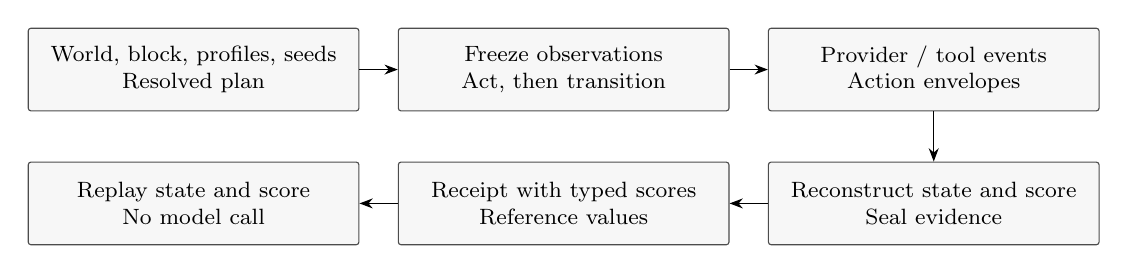
\begin{tikzpicture}[box/.style={draw=black!70, fill=black!3, rounded corners=1pt, minimum width=4.2cm,
  minimum height=1.05cm, align=center, font=\footnotesize}, >=Stealth]
\node[box] (a) at (0,0) {World, block, profiles, seeds\\Resolved plan};
\node[box] (b) at (4.7,0) {Freeze observations\\Act, then transition};
\node[box] (c) at (9.4,0) {Provider / tool events\\Action envelopes};
\node[box] (d) at (9.4,-1.7) {Reconstruct state and score\\Seal evidence};
\node[box] (e) at (4.7,-1.7) {Receipt with typed scores\\Reference values};
\node[box] (f) at (0,-1.7) {Replay state and score\\No model call};
\draw[->] (a) -- (b); \draw[->] (b) -- (c); \draw[->] (c) -- (d); \draw[->] (d) -- (e); \draw[->] (e) -- (f);
\end{tikzpicture}
\caption{Execution and receipt path.}
\label{fig:runtime}
\end{figure}

For simultaneous play, observations are frozen before requesting any
action, and the family receives the joint action set. This prevents a
seat from observing a peer's same-phase action through request order;
order effects inside the family transition remain the family's
responsibility. Parsing and legality failures retain typed reasons.
The declared invalid-action policy either stops execution or passes an
invalid envelope to the family for its stated consequence. A family-hook
exception is a defect in the evaluation apparatus, not a subject score.

Each attempt has an append-only event log and content-addressed artifacts.
Instrumented calls record a start before dispatch and a terminal outcome;
actions, transitions and termination are also recorded. Finalization
reconciles these records, reconstructs scoring input, invokes the scorer
and seals the evidence before writing a receipt. Retries follow the
declared conditions and limits. The October path rejects empty replies and
incomplete truncated answers before family parsing; older executors can
differ. These guarantees cover the interfaces actually used by the driver.

\subsection{Scoring, replay and access}
\label{app:runtime-replay}

A receipt binds the plan, world, cell, attempt, declared per-seat profile
hashes, implementation pins and evidence seal to typed score records.
Measurement validity and inclusion in analysis are separate statuses.
Each score records its metric, reference type, scope, direction and native
units. Declared applicable metrics must be returned; deferred and
inapplicable metrics are listed separately. Deferred metrics cannot serve
as the primary score. At most one receipt is included per planned cell,
but this cardinality check cannot establish that attempt selection
preceded observation of the outcome.

Replay uses the family's state-transition and scoring hooks with recorded
actions and compares reconstructed states and receipt scores. It reads
the stored observation, response, parse result and legality result; it
does not rerun the model, harness or parser. Completed scored executions
carry \texttt{state\_\allowbreak{}and\_\allowbreak{}score}, including those excluded as invalid
measurements. Operational-failure receipts carry \texttt{none} and are
verified as exclusions. Replay neither converts an exclusion into a
successful episode nor certifies an analysis outside the receipt.

At the October baseline, the reviewer command is:
\begin{verbatim}
aeread verify-replay BUNDLE --run-root R \
  --setup MODULE:CALLABLE
\end{verbatim}
It checks published bindings against retained run evidence and reports
verified, differing or missing-evidence rows. Coverage extends to every
published episode only when the bundle identifies that trajectory grain;
otherwise it covers the receipts found under the run root. Having this
command available does not establish that it was run on a given panel.

Public live bundles contain sanitized receipt projections and digests;
the baseline policy omits full prompts, raw responses, model reasoning,
complete live receipts and failure messages. Independent replay therefore
also requires retained run roots. A digest cannot recover omitted inputs.
Appendix G records access limits, and Table~\ref{tab:case-paths} separates
inline checks, later audits and headline-score reconstruction. Seeds and
sealed requests support reconstruction of recorded play, without
guaranteeing a fresh model response \citep{he2025nondeterminism}.

\subsection{Applied controls and experimental coverage}
\label{app:runtime-cases}

The API and CLI paths do not apply the same controls. Table~\ref{tab:cli-controls}
summarizes the CLI subjects in the reviewed case studies. The OpenRouter
client checks reported model and route information against the declared
pin, but cannot independently attest the hosted deployment or whether a
requested seed or reasoning control was honored. Reasoning-effort labels
are not a common scale of deliberation across models.

\begin{longtable}{@{}P{1.25in}P{2.6in}P{2.6in}@{}}
\caption{CLI controls applied in the reviewed panels. These describe
the evaluated subjects, not all capabilities of the products.}
\label{tab:cli-controls}\\
\toprule
\textbf{Control} & \textbf{Claude Code / Opus 5.5} & \textbf{Codex CLI / Sol 6.1}\\
\midrule\endfirsthead
\endhead\endfoot\endlastfoot
Client and execution & Kernel \texttt{ClaudeCodePrintClient}; one ephemeral process per action; low effort. & External \texttt{CodexExecClient}; one ephemeral process per action; low effort.\\
Sampling and output & Seed, temperature and output-token limits not applied. & Seed, temperature and output-token limits not applied.\\
Tools and session & Tools disabled; no persistent session. & Tool definitions retained; a call using a tool is refused.\\
Observed identity & Version 2.1.292; binary digest \texttt{97a01e5b}, rechecked before calls. & Version 0.160.0; binary digest \texttt{112fae7a}; no served-model identity.\\
Accounting limits & Two internal model turns observed per kernel call; internal retries are not separate kernel attempts. & Adapter digest \texttt{3f254873}; CLI internal execution is not independently certified.\\
User customizations & \verb|--safe-mode|: no CLAUDE.md, memory, skill, plugin, hook, output style or MCP server reached the model. The run's working directory, a repository checkout, and the account's email address were in context. & \verb|--ignore-user-config| did not remove the operator's skills: eight were listed beside Codex's four built-in ones (about 500 input tokens a call), two described in benchmark and evaluation terms. The working directory's name contained the project's name.\\
Shared limits & Working directory and environment unsealed; costs estimated at list prices. & Working directory and environment unsealed; costs estimated at list prices.\\
\end{longtable}


Table~\ref{tab:cli-controls} describes the first agreement confirmatory. The
second isolated both tools and probed their context before and during its
runs, and every probe was clean (Section~\ref{sec:cases}).

Table~\ref{tab:case-paths} identifies the paths behind the reported
results. The October executor digest prefix is \texttt{607a79ce}; the September prefix is
\texttt{3cd3278c}.

\renewcommand{\thetable}{H.2}
\begingroup
\small
\setlength{\tabcolsep}{4pt}
\renewcommand{\arraystretch}{1.16}
\begin{longtable}{@{}P{1.28in}P{2.18in}P{3.06in}@{}}
\caption{What produced the case-study numbers. Inline replay, a later audit and
headline-measure reconstruction are separate checks.}
\label{tab:case-paths}\\
\toprule
\textbf{Panel} & \textbf{Executor, driver and client} & \textbf{Receipt audit and headline coverage}\\
\midrule\endfirsthead
\multicolumn{3}{@{}l}{\textit{Table \thetable\ continued: experimental execution paths}}\\
\toprule
\textbf{Panel} & \textbf{Executor, driver and client} & \textbf{Receipt audit and headline coverage}\\
\midrule\endhead
\midrule\multicolumn{3}{r}{\textit{Continued on the next page}}\\\endfoot
\bottomrule\endlastfoot
Housing v14\newline 1,800 planned cells; separate 48-cell fill
& October executor \texttt{607a79ce}; run 6 October. Family price driver; OpenRouter on pinned routes, through the seat router; minimal-chat harness.
& Original panel: 1,764 completed receipts and 36 operational-failure receipts. Inline replay, then bundle replay of 600 rows per model (564 scored for Gemini), and 48 fill rows. The receipt scores six tenants. The separately versioned seat-0 reanalysis was re-extracted from sealed records and regenerated exactly on 16 October.\\
\addlinespace[4pt]
Housing CLI\newline 20 worlds, 40 cells per subject
& October executor \texttt{607a79ce}; \texttt{housing\_\allowbreak{}cli.\allowbreak{}py}. Claude Code and the external Codex client use the same seat router.
& 40 completed cells per subject; inline receipt replay only. No published bundle or independent bundle-audit report in the review. Inherits Housing's seat and headline-score gaps. The driver is not digested in the plan.\\
\addlinespace[4pt]
Procurement CLI\newline 24 worlds, two briefs, two subjects
& October executor \texttt{607a79ce}; \texttt{procurement\_\allowbreak{}cli.\allowbreak{}py}; runs on 9 October. Same CLI clients as Housing.
& 24 receipts per run root. On 16 October, all 96 CLI receipts across both briefs passed state and score audit; a source-pinned derivation from sealed actions reproduced every decision loss. Historical receipts still score contribution margin. Full run roots are retained.\\
\addlinespace[4pt]
Procurement flash\newline 24 worlds per model
& October kernel; \texttt{pay\_\allowbreak{}or\_\allowbreak{}test\_\allowbreak{}openrouter.\allowbreak{}py}, digest \texttt{f5ec607c}. Runs 13 October; the driver bytes match its committed version. Pinned OpenRouter clients.
& 24 completed receipts per model; 72 and 76 provider calls. On 16 October, all 48 receipts passed state and score audit and the pinned sealed-action derivation reproduced every decision loss. Table E.14's means and intervals are unchanged.\\
\addlinespace[4pt]
Data-center agreement\newline development and confirmatories
& Development: September executor \texttt{3cd3278c}; \texttt{agreement\_\allowbreak{}cli.\allowbreak{}py}. Confirmatory v1: \texttt{agreement\_\allowbreak{}confirmatory\_\allowbreak{}cli.\allowbreak{}py}, frozen plans, CLI versions and limits. Confirmatory v2 (Table 5.4): \texttt{agreement\_\allowbreak{}confirmatory\_\allowbreak{}v2\_\allowbreak{}cli.\allowbreak{}py} on v1's pieces, with isolation probes from \texttt{cli\_\allowbreak{}isolation.\allowbreak{}py}.
& Development: 2,417 valid of 2,456, inline replay. Confirmatory v1 plus pilot: 1,175 valid of 1,176; another 120 scripted dry runs. All 1,295 scored receipts replay offline; one excluded receipt has a separate digest/seal check. Confirmatory v2: 640 valid of 640, every receipt replayed offline from its sealed events. Earnings and IR violations are receipt leaves.\\
\addlinespace[4pt]
Refund V2.1\newline four models, 120 cells each in the reported panel
& September kernel; \texttt{v2\_runner}; Arena client. Contributed registration calls the shared executor and finalizer.
& Published projections carry \texttt{state\_\allowbreak{}and\_\allowbreak{}score}; inline replay. Gap figures are regenerated by \texttt{v2\_\allowbreak{}gap --check}. Produces kernel receipts despite being outside the trusted scoring-contract fixture.\\
\addlinespace[4pt]
Refund V2.5\newline 816 provider-free trajectories
& A Refund release on the October runtime, without kernel changes. Contributed QC path; all seats use a scripted provider; paid calls refused.
& Release replays and audits all 816 receipts. No published bundle in the review. These runs qualify release conformance, not paid-model performance; they do not replace the V2.1 results.\\
\end{longtable}
\endgroup


\paragraph{Housing: seat attribution and headline measure.}
The v14 plan names the subject profile for all six tenant seats, while
the driver-side \texttt{SeatRouterClient} supplies scripts for seats 1--5.
The realized routing map is retained in an unsealed side log.
The original receipt scores the six-tenant sum, while the headline
concerns seat 0. The original headline reads outcome facts
copied into a separate unsealed result file. The later
\texttt{price\_\allowbreak{}reply\_\allowbreak{}posterior} analysis derives its
corrected measure from sealed events. On 16 October, its trajectory table
was re-extracted from the original sealed run roots and the committed
analysis regenerated exactly. This remains a post-run, separately
versioned derivation; the original receipt's certificate is unchanged.

\paragraph{Procurement: the decision-loss reference.}
The receipt scores contribution margin and regret against a
full-information bound. Headline decision loss instead uses the optimal
policy under the buyer's information. The original report replayed an
\texttt{action\_\allowbreak{}trace} copied into an unsealed result row through an unpinned
\texttt{pay\_\allowbreak{}or\_\allowbreak{}test\_\allowbreak{}reference}. On 16 October, a separate
\texttt{pay\_\allowbreak{}or\_\allowbreak{}test\_\allowbreak{}reanalysis} audited all 144 original receipts through
state and score replay, extracted parsed actions and validity from sealed
events, and recomputed every loss with a source-pinned reference. The 96
final-brief results and 48 earlier-brief results match; preserving the
original bootstrap order also reproduces Table E.14's intervals. The
accompanying projection permits headline recomputation without private
run roots, while re-auditing the original logs still requires them.
This resolves the reported panels' derivation gap. It does not add a
decision-loss leaf to their historical receipts or implement the
prospective case-interface standardization that has been proposed.

\subsection{Scope and remaining limits}
\label{app:runtime-limits}

The kernel supplies neither a sandbox nor complete mediation of external
activity: families and tools can run outside its ports. Resume checks and
continues a valid log, but a hard kill can leave an unmatched call start
that cannot be finalized. An outcome-unknown record does not prove
whether an external side effect occurred. Hosted-model determinism and
arbitrary-crash recovery are not claimed.

Campaign stopping and spend accounting also depend on the driver.
At the reviewed baseline no family driver used the kernel's optional
consecutive-failure halt helper, and there was no kernel-wide campaign
cost circuit breaker. The later agreement confirmatory driver froze its
own five-failure halt, list-price cap and wall-time ceiling; none fired. Housing used worker-level stop rules; twelve
workers account for its 36 refused cells. The event-log spend reader
distinguishes exact from incomplete totals, but had not been adopted by
family drivers; CLI list-price estimates remain separate from billed
charges. The inclusion rule does not prove pre-outcome attempt selection.

Integration and scientific qualification are distinct. The 21-package
inventory includes wrappers, re-implementations and native packages with
different fidelity, fixture and live-run coverage. The supplement retains
those distinctions and the incomplete implementation-review status;
package counts and passing tests do not establish case validity.
Section 6 and Appendix F give the applied QC evidence and incident
history. None of the four designs fully passes Gates 1--5 in this review,
and later checks or repairs do not retroactively qualify earlier runs.

\end{document}
